\documentclass{article}
\usepackage{graphicx}
\graphicspath{ {graphs/} }
\usepackage{geometry}
\geometry{a4paper, portrait, margin=1.0in}
\usepackage{gensymb}
\usepackage{booktabs}
\usepackage{amsfonts}
\usepackage{pgfplotstable, booktabs}

\pgfplotstableset{
  	every head row/.style={before row=\toprule,after row=\midrule},
    every last row/.style={after row=\bottomrule}
	}

\begin{document}
\begin{titlepage}
    \begin{center}
        \vspace*{1cm}
        
        \Huge
        \textbf{Reconstruction of Charge Number of Heavy Cosmic Rays using Cherenkov Light}
        
        \LARGE
        
        \vspace{1cm}
        
        \textbf{Robert Stein}\\
        \textbf{CID 00819615}
        
        \vspace{1cm}
        
\includegraphics[width=0.4\textwidth]{Imperial_College_London_logo} 
        \hspace{0.5cm}
        
\includegraphics[width=0.4\textwidth]{hamburglogo}
        
        \vspace{1cm}
        
        Supervisor: Professor Dieter Horns
        
        \large
        \vspace{1.0cm}
        
        A thesis presented for the degree of\\
        \textbf{Master in Science}
        
        \vspace{0.5cm}

        Physics Department\\
        Imperial College London
        
        \vspace{0.5cm}
        
        \today
        
    \end{center}
\end{titlepage}
\section*{Abstract}
Between impact with the upper atmosphere and decay into a charged particle shower, heavy cosmic ray elements such as Iron emit Cherenkov Light at an angle determined by the Refractive Index of the air and the energy per nucleon. This direct Cherenkov Light forms a characteristic circular light distribution on the Earth's surface with an intensity proportional to the square of the cosmic ray charge. A new method has been developed to reconstruct this charge number, by fitting the received Cherenkov Photons to the characteristic Lateral Photon Distribution. The expected performance for various existing and planned installations will be discussed.

\section*{Zusammenfassung}
Between impact with the upper atmosphere and decay into a charged particle shower, heavy cosmic ray elements such as Iron emit Cherenkov Light at an angle determined by the Refractive Index of the air and the energy per nucleon. This direct Cherenkov Light forms a characteristic circular light distribution on the Earth's surface with an intensity proportional to the square of the cosmic ray charge. A new method has been developed to reconstruct this charge number, by fitting the received Cherenkov Photons to the characteristic Lateral Photon Distribution. The expected performance for various existing and planned installations will be discussed.
\newpage
\tableofcontents
\newpage

\section{Preface}
The basis of this thesis work can be divided into two halves. The first half is the simulation of cosmic ray HESS camera images, and analysis work based on these images. The second half is a Monte Carlo study simulating air shower intensities, based entirely on function fitted from the HESS camera images. 

It is important to note that the simulation of cosmic ray air showers for the first part of my thesis was performed using the CORSIKA software \cite{Heck98}, and the resultant HESS camera images were produced using the Sim\textunderscore Tel array software \cite{Bernlohr08}. I claim no credit for the complex simulations that these packages have enabled me to perform. 

Additionally, a significant portion of this work relies on Supervised machine learning that was performed using the SciKit learn package \cite{scikit-learn}. Although I wrote the relevant Python scripts to facilitate data categorisation and algorithm training, the package acts as a black box to convert training data into a functioning Boosted Decision Tree. I would like to make clear that I am indebted to those who produced this package, without whom this analysis could not have been performed.

Aside from this, all other work in this thesis is my own. I wrote all necessary code for the Monte Carlo simulation, and it was conducted entirely by me. Similarly 

Thank Dieter, and Attilla, and...
\newpage

\section{Introduction}
Cosmic Rays are abundant in our galaxy, and enter the Earth's upper atmosphere from every direction. Their flux is governed by a well-defined energy power law, which is almost unchanged across more than 10 orders of magnitude \cite{Blasi:2013rva}. Cosmic Rays are in fact not rays but rather charged particles, primarily protons, which have been accelerated by various galactic or stellar processes. The exact cosmic ray composition is energy dependent, and provides information regarding the source of cosmic rays. Heavy cosmic rays, the most common of which is iron, vary substantially in relative abundance for different energy scales.

Being highly-energetic charged particles, Cosmic rays will often travel through the atmosphere faster than the local speed of light. Consequently, many Cosmic Rays will emit Cherenkov light over substantial distances, and this light will be visible on the ground. There are numerous Telescope Arrays which image the Cherenkov Light emitted by Cosmic Rays in the atmosphere, including the HESS, MAGIC and VERITAS Experiments. Although the number of emitted photons is comparatively small, the Cherenkov light is still brighter than the night sky background because the telescopes are able to capture images with an exceptionally short recording time, equal to 80ns for the HESS array \cite{Funk:2004ie}. The Cherenkov photons all arrive almost simultaneously, so have a high intensity over the short time window during which the image is formed.

All telescope arrays rely on Hillas Analysis with extracted parameters from each of the camera images being used to reconstruct the events, but heavy atmospheric blurring means that charge resolution is very poor. For Iron Nucleus events, we would expect to reconstruct \[Z \approx 26 \pm 5 \] with a core position resolution of roughly $d \approx 20 m $ \cite{hess07}. The Cosmic Rays imaged by these telescopes have energies between $13-200 $TeV, and at present, no study of the relative abundance of different cosmic ray elemental abundances exists at these energies. If the telescope arrays could be used to spectroscopically analyse the Cosmic rays, it could provide important clues regarding the mechanism of Cosmic Ray formation and propagation in the galaxy. However, current charge resolution from Hillas Analysis is not small enough to undertake such a study. The principal goal of this thesis is to enable spectroscopic analysis with Cherenkov Telescope arrays, by improving the charge resolution of reconstructed events.

A theoretical study by Kieda in 2001 \cite{kieda01} suggested that for a core position resolution of $d \approx 5 $ m, we could expect to see a charge resolution of $ \sigma_{Z} \approx 1 $ for elements of $Z = 20$ or higher. In this case the core position resolution would be the limiting value. Thus, if the LPD method can achieve this core position resolution, the precision will be sufficient to extract the abundances of the different Cosmic Ray Elements. 

Instead of Hillas Analysis, we will consider a new method for event reconstruction, in which we fit the known Direct Cherenkov (DC) Light observed by each telescope to a characteristic Lateral Photon Distribution (LPD) function. This new technique is valid both for currently running experiments, as well as planned experiments such as the Cherenkov Telescope Array (CTA). It uses only the information from the DC Pixel identified in the shower images. Possible improvement in core resolution is the prime motivation for the new LPD technique.

To understand why an LPD exists, it is important to recall that Cherenkov emission begins when a charged particle passes the local speed of light in a medium.  We know that the refractive index of air is proportional to the density of air. Thus, the minimum velocity needed for Cherenkov Emission is lower for low atmospheric altitudes, because the air is denser. If the velocity is sufficient, we will observe photon emission from the particle at the Cherenkov Angle $\theta_{c}$.

\[ \cos(\theta_{c}) = \frac{1}{\eta \beta}  \Longrightarrow \beta_{min} \geq \frac{1}{\eta}\]

We obviously require that the Cherenkov Angle is real, so then require $\cos(\theta_{c}) \leq 1$. The minimum required velocity $\beta_{min}$ is thus equal to the inverse of the local refractive index $\eta$. The velocity of a particle is a function of its energy, determined with the relations $\gamma = \frac{E}{m_{0} c^{2}}$ and $\beta^{2} = 1 - \frac{1}{\gamma ^{2}}$. Thus, we find that the minimum velocity ultimately leads to an Energy per unit mass threshold. If we assume that the slight difference in proton and neutron mass is negligible here, than we can determine a local energy per nucleon threshold that will be valid for all Cosmic Rays passing a given atmospheric altitude. 

The Energy per Nucleon Threshold for Cherenkov Light Emission as a function of height is illustrated in \ref{fig:generalenergy}. Once the Energy of a Cosmic Ray exceeds the local Cherenkov Energy Threshold of the atmosphere, the Nucleus will begin emitting a ring of Cherenkov Light.  Then for a given Telescope Array altitude above sea level and a given height h, simple trigonometry yields the final radius of emission on the ground:
\[ Radius(h) = \tan (\theta_{C}(h)) \times (h - altitude_{array})\]

The refractive index as a function of height is shown in as seen in Figure \ref{fig:lpd}, using standard values listed in the appendix. Because the refractive index of air increases very quickly as the height decreases, the Cherenkov Angle $\theta_{C}$ will also increase rapidly with decreasing height. Thus, although the displacement $(h - altitude_{array})$ decreases as the height, the radius on the ground increases as height decreases. Consequently the upper atmosphere emission contributes to the inner LDF, while the lower atmosphere emission contributes to the outer LDF. As the cosmic ray travels down through the atmosphere, Cherenkov Emission continuously illuminates new areas on the ground that were previously unlit, without re-illuminating inner regions. 

Emission continues until the first interaction with the atmosphere, occurring at a randomly distributed height we call $h_{int}$. The maximum radius of the DC light will then be $r_{max} = Radius(h_{int})$. This is extremely useful, because for all distances up to $r_{max}$, the LPD will be completely independent of the emission height. One full parameterisation of the LPD will thus be valid for all heights, provided the maximum radius is known.

Above threshold, Cherenkov Emission is determined by the Frank Tamm formula \cite{ppreview}.  Under the assumption of constant magnetic permittivity and a zenith angle of $90\degree$, and with  the vertical distance travelled in meters $\Delta_{h}$ and the emission energy range in eV $\Delta_{E}$, we can find an approximate Cherenkov Emission formula.
\[ \frac{d^{2}N_{photons}}{dEdh} = \frac{\alpha Z^{2}}{\hbar c} \sin^{2} \theta_{c}(E) \approx 370 Z^{2} \sin^{2} \theta_{c}(E)\, cm^{-1}eV^{-1} \]

\[ N_{photons} \approx (37000 \times Z^{2} \times \Delta_{h} \times \Delta_{E}(E))\, m^{-1}eV^{-1}\]
 
A full simulation of the LPD was undertaken, with the assumption that $\Delta_{E} \approx 0.7$ independent of Energy. Although this is certainly an oversimplification of the true picture, it will allow us to understand the variation of the LPD with height. A more rigorous LPD parameterisation will be found later to account for the dependence of $\Delta_{E}$ on the Energy. 

If we divide the number of emitted photons by the area of the annulus between the ring radii at $h$ and $h - \Delta_{h}$, we retrieve the LDF shown in \ref{fig:lpd}, which varies with $ \rho_{DC}  = f(r) \times Z^{2}$ . Thus the amplitude of the LDF is proportional to the square of the Cosmic Ray charge, enabling us to reconstruct this number from the DC emission. This proportionality is the basis for charge reconstruction in the LDF method.

\begin{figure}
\begin{center}
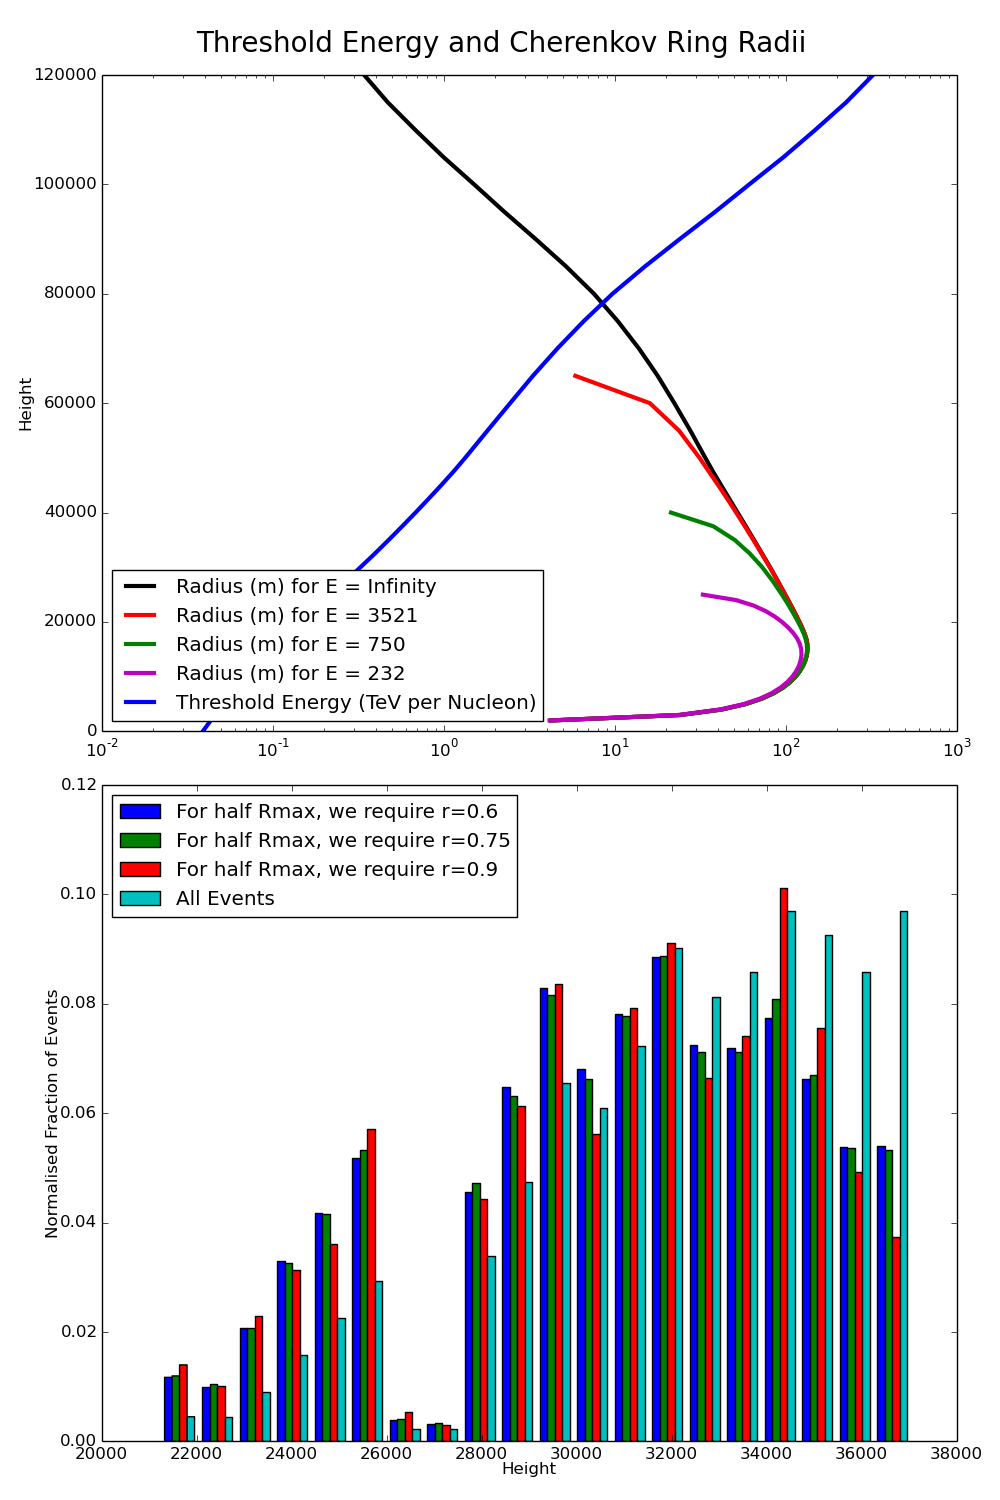
\includegraphics[height=0.9\textheight]{logenergyradius}
\caption{The Threshold Energy for Cherenkov Emission is marked in blue. With the assumption of $\beta=1$, the maximum emission radius is marked in black. The red and green and magenta line show the emission radius at 3.57 and 0.75 and 0.23 TeV per Nucleon respectively. The Green line is sufficiently close to the background to be saturated at 24km, while the magenta line is not.}
\label{fig:generalenergy}
\end{center}
\end{figure}

\begin{figure}
\begin{center}
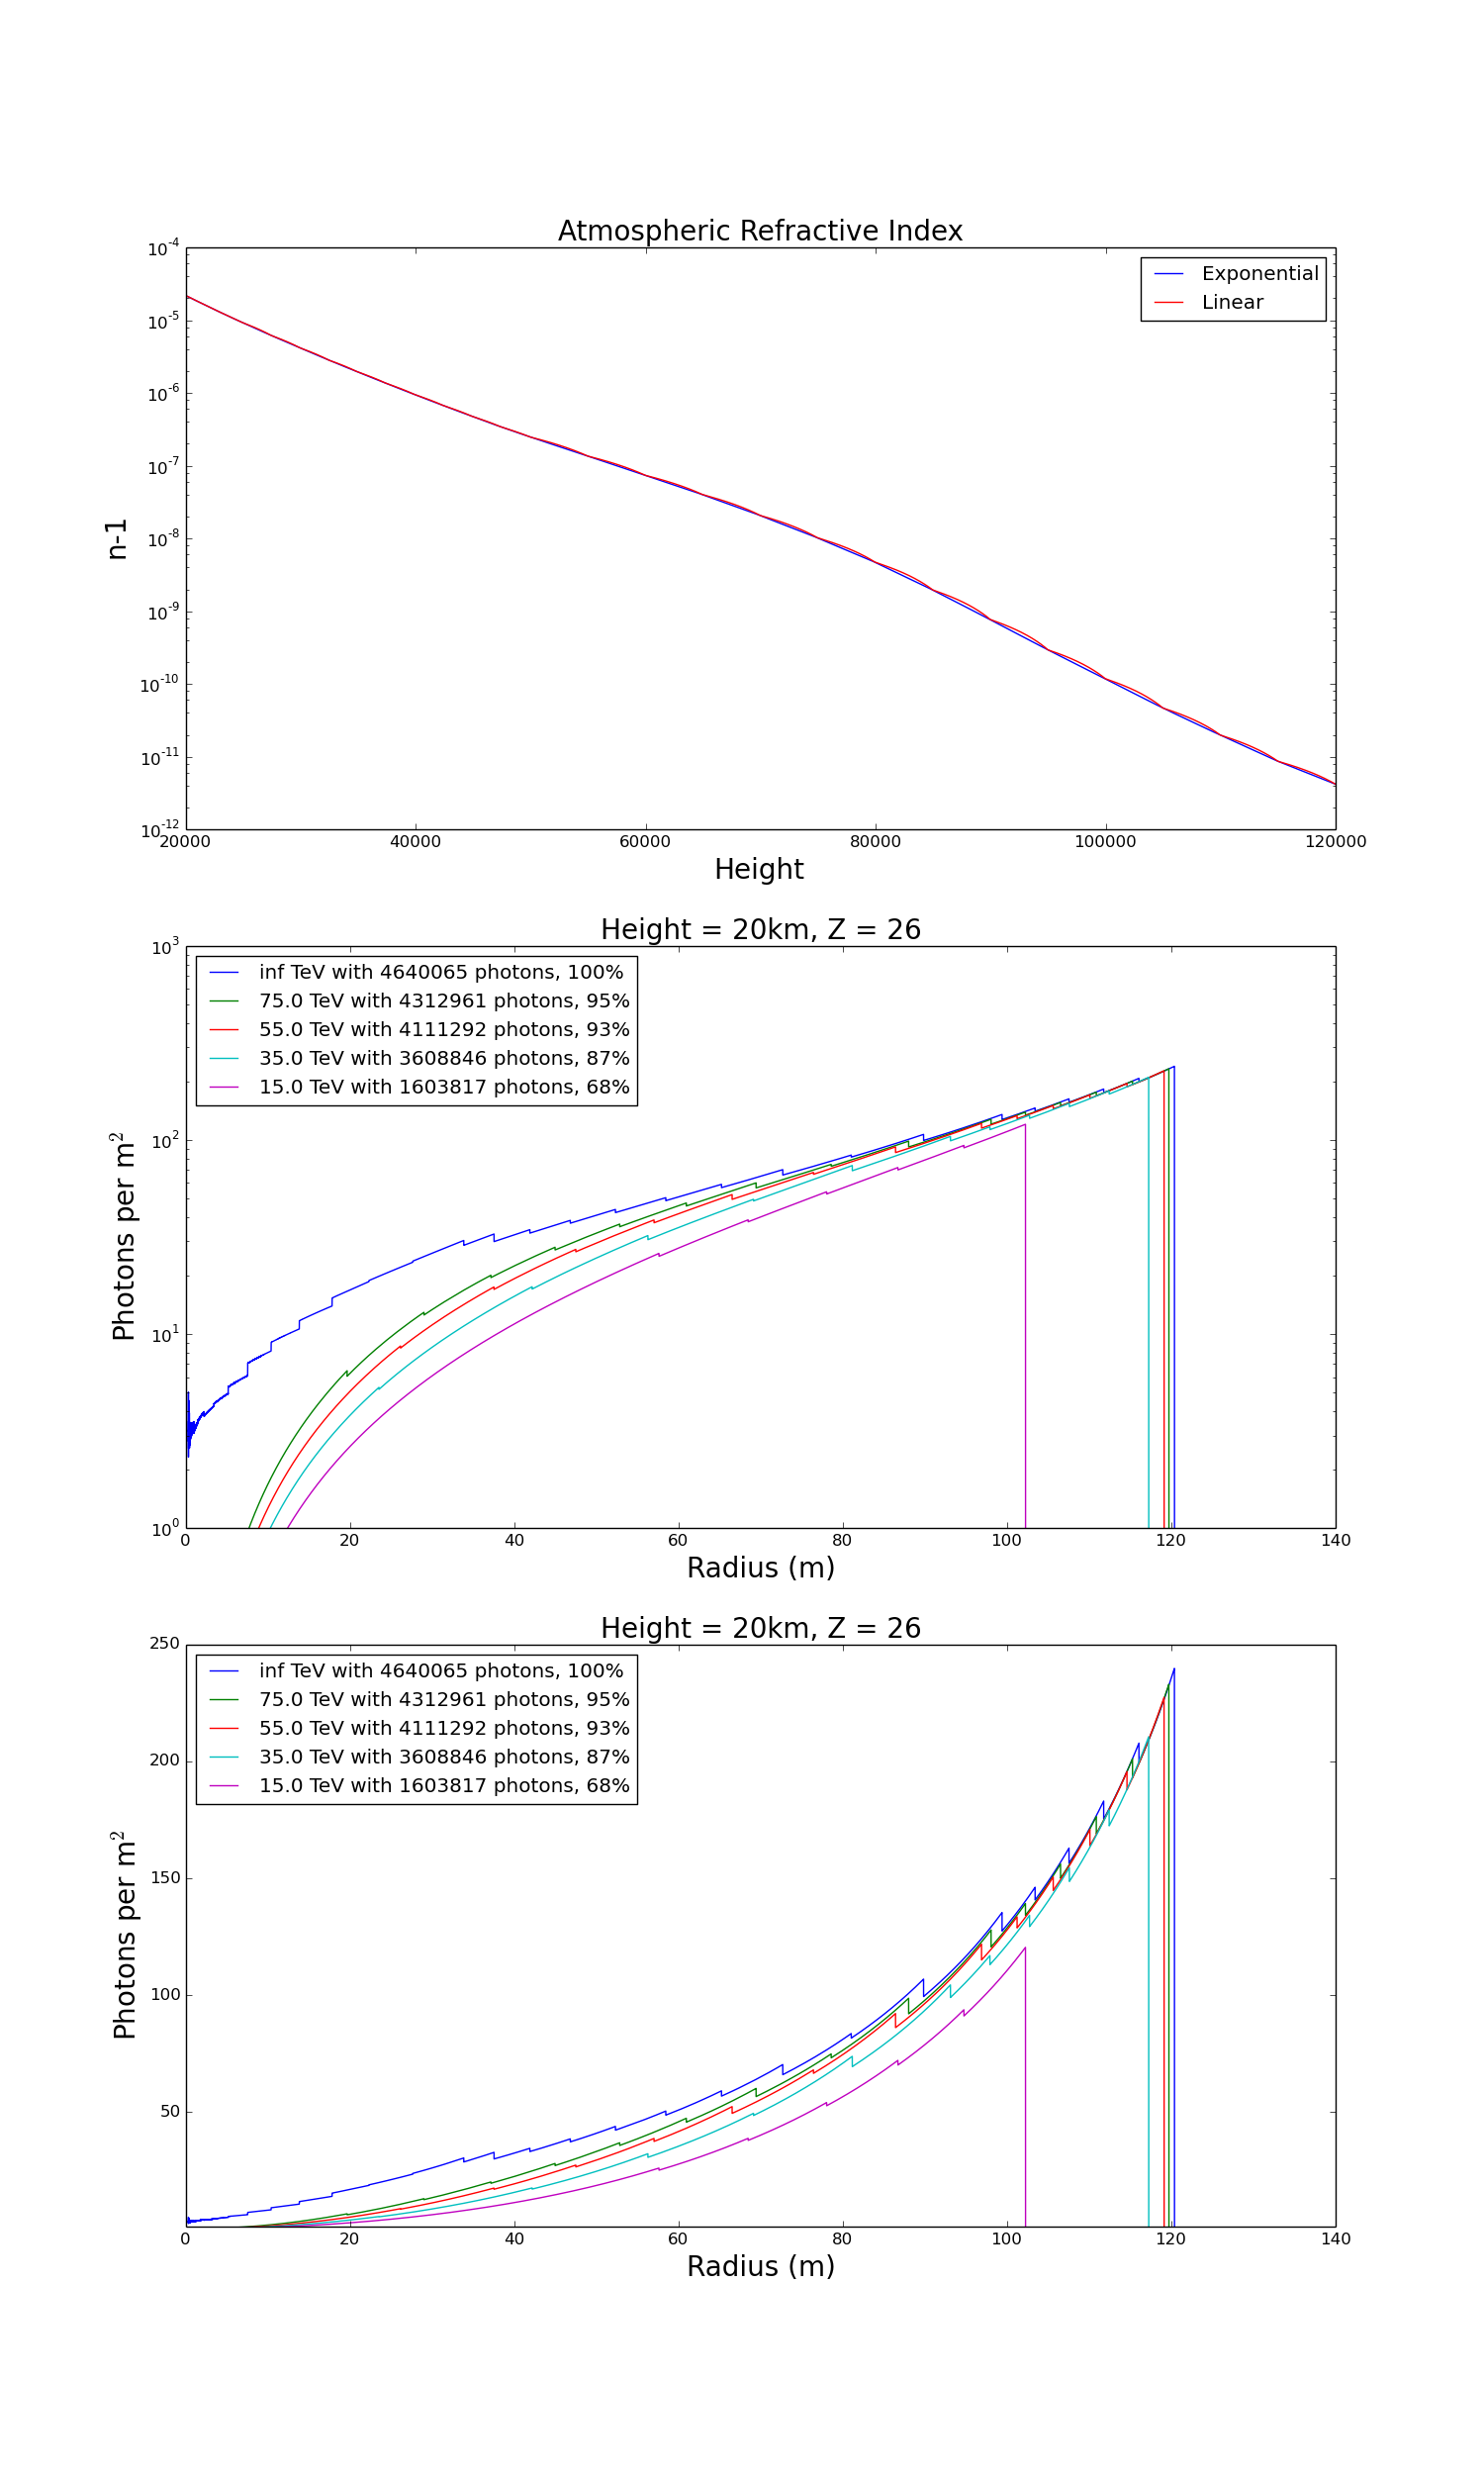
\includegraphics[height=0.9\textheight]{simulatedlpd}
\caption{Above, the refractive index is shown with both linear and exponential interpolation between the known values. The LPD obtained from simulation of an Iron Nucleus up to a first interaction height of 25km for a range of Core Energies. An altitude of 1.8km for the experimental array is assumed. Atmospheric absorption, although neglected, is broadly constant across the emission range leading to uniform amplitude scaling.}
\label{fig:lpd}
\end{center}
\end{figure}

The refractive index at a series of heights, based on data from the HESS site, is shown \ref{fig:lpd}. Exponentials are fitted between points to provide interpolation, and a comparison can be made to a linear interpolation that is also plotted. Despite the exponential interpolation, discontinuities in the second derivative of the refractive index prevent the LPD from being smooth in the simulation. This is unimportant, because in reality the variation due to atmospheric conditions and random noise will smear out any discontinuities in the LDF.

We can also see ground emission radius as a function of height in Figure \ref{fig:generalenergy}. We find that the high-radius emission (occurring near the first interaction region) varies little between different high energies. We deem this to be \textquoteleft Saturated Emission\textquoteright. To accurately quantify Saturated Emission, we can compare the photon density to the theoretical maximum photon density, corresponding to an infinite-energy particle with $\beta =1$ in Figure \ref{fig:lpd}. The illustrated maximum is useful as a reference, although because the atmosphere is not modelled beyond an altitude of 120km, the small-radius emission is not accurately simulated entirely correctly. However, real cosmic rays in the considered energy regime will all cross the emission threshold and begin emission at an altitude much lower than 120km, so can be considered accurately modelled.

The salient point is that there is a clear characteristic photon distribution that, for energies above 25 TeV at least, is almost constant except for a varying endpoint. However, we will not be able to directly measure this LPD. Instead, a telescope images containing air showers must be analysed, and from these images, we can infer the quantity of DC light present amongst a large degree of background. Extensive simulations of Camera images will be performed, in order to quantify the resultant LPD extracted from the telescope images. After determining a likely experimental LPD, Monte Carlo events can be simulated, and then reconstructed. 

To reconstruct an event, we will need to find the \textquoteleft Core position' of the Cosmic Ray, which is defined as the position on the ground through which the Cosmic Ray would pass if it continued in a straight line to the ground. In addition, we will need to determine the Energy, first interaction height, and the charge. We would normally require at least five data points in order to reconstruct these variables. However, it is possible to use the non-observation of light in one telescope to constrain the core position. Thus, we require that an  event was be seen by at least four telescopes for a five-telescope array such as HESS. 

\section{DC Pixel Identification}
\textbf{Cosmic Rays will emit Direct Cherenkov (DC) light in the upper atmosphere, before generating an Extended Air Shower (EAS) through interaction with the lower atmosphere. }

In telescope images, the DC light is usually concentrated in a single  \textquoteleft DC pixel'. Identifying this pixel is challenging, because the brighter EAS Cherenkov light background often overlaps with the DC pixel. In order to apply the LPD method to data, we must first identify the DC pixel in a shower image, and determine the number of DC photoelectrons present. 

We define the variable $Q_{DC} = \frac{Intensity_{N.N.max}}{Intensity}$ as the ratio of the largest neighbouring pixel intensity to the intensity of a given pixel. In previous experiments, the DC pixel candidate was identified by applying a number of cuts to pixels in an image \cite{hess07}, and from the subset of pixels passing the specified cuts, selecting the pixel with the smallest $Q_{DC}$ as the \textquoteleft DC candidate'. Due to the low pass rate for cuts, we obtain a small low-contamination dataset, while the majority of telescope images are left without a DC pixel candidate. An improved method would aim to increase the number of correctly identified DC pixels, while still enabling cuts which discriminate well between correctly and incorrectly identified DC pixels.

Classifiers provide an alternative method of identification, making use of supervised machine learning to find rules for categorising pixels. To train a classifier, we require a set of training pixels, as well as the correct class for each pixel. Once trained, a classifier can then be used to predict the class of a pixel.

The CORSIKA package \cite{Heck98} was used to generate Cosmic Ray events, and the Sim\textunderscore telarray package  \cite{Bernlohr08} was used to generate corresponding HESS array telescope images.  Simulation with EAS background was used to produce training pixel sets, while corresponding simulation without EAS background was used to find the true DC pixel in each training image. As part of a new method developed for this analysis, a Boosted Decision Tree (BDT) classifier was trained with the data to identify DC pixels. Once trained, the BDT was applied to a separate \textquoteleft testing' set of simulated telescope images. As before, the true DC pixel was determined from a second EAS-free simulation. Thus, the accuracy of BDT identification for test telescope images was calculated.

\subsection{Image Simulation}
The full simulation of air showers was performed using the CORSIKA package, with a standard atmospheric profile derived from measurements conducted at the HESS site in Namibia. In total, 5000 training events and a further 10000 testing events were simulated. The simulated particles were $Fe^{56}$, within the Energy Range of $35-135$ TeV and a spectrum $\phi(E) \propto E^{-2.7}$. For each set of simulated event, 4 unique random number seeds were used to generate the shower. An altitude of 1800m was assumed, again corresponding to the HESS site. The simulated zenith angle ranged from $0\degree < \theta < 2 \degree$, while the simulated azimuth angle ranges from $-2\degree < \phi < 2 \degree$. The four smaller HESS-phase-1 telescopes were arranged in a cross along the x/y axis with the larger HESS-phase-2 \textquoteleft CT5' telescope placed at the center. The length of each cross arm was $85m$. The simulated target region of the cores was chosen to be a square centered on CT5, with each 300m-long side bisecting the x/y axis.Due to hardware differences between CT5 and the original HESS 1 telescopes, we analyse HESS1 and HESS2 images separately. To determine the true class of each pixel, a simulation was initially run with an energy cut of 10 PeV on all muons and electrons. Because this cut exceeded the primary particle energy, neither daughter muons and electrons, nor the photons they would have emitted, were simulated. Thus the hadronic Cherenkov Light from the primary particle and daughter fragments, but not the EAS light, was present in the camera image. A second identical \textquoteleft EAS Simulation' was run including the same random seeds, but without the energy cut on muons and electrons. This gave a complete EAS image including identical DC light.

With the sim\textunderscore telarray package, the expected HESS hardware response to each air shower was simulated. Among other things, the program accounts for atmospheric transmission and density, mirror positions, sizes and reflectivities, camera shadowing and triggering, quantum efficiency and pulse responses. For the full-shower image, the night sky background was also simulated by sim\textunderscore telarray. Due to the comprehensive and detailed nature of these hardware simulations, the resultant images can be considered \textquoteleft realistic'.  However, sim\textunderscore telarray introduces various sources of random noise to the simulation, leading to some divergence in the DC light between the EAS-free and full-shower images.

\begin{figure}
\newgeometry{a4paper, portrait, margin=1.5in}
\centering
\begin{minipage}{0.45\textwidth}
\centering
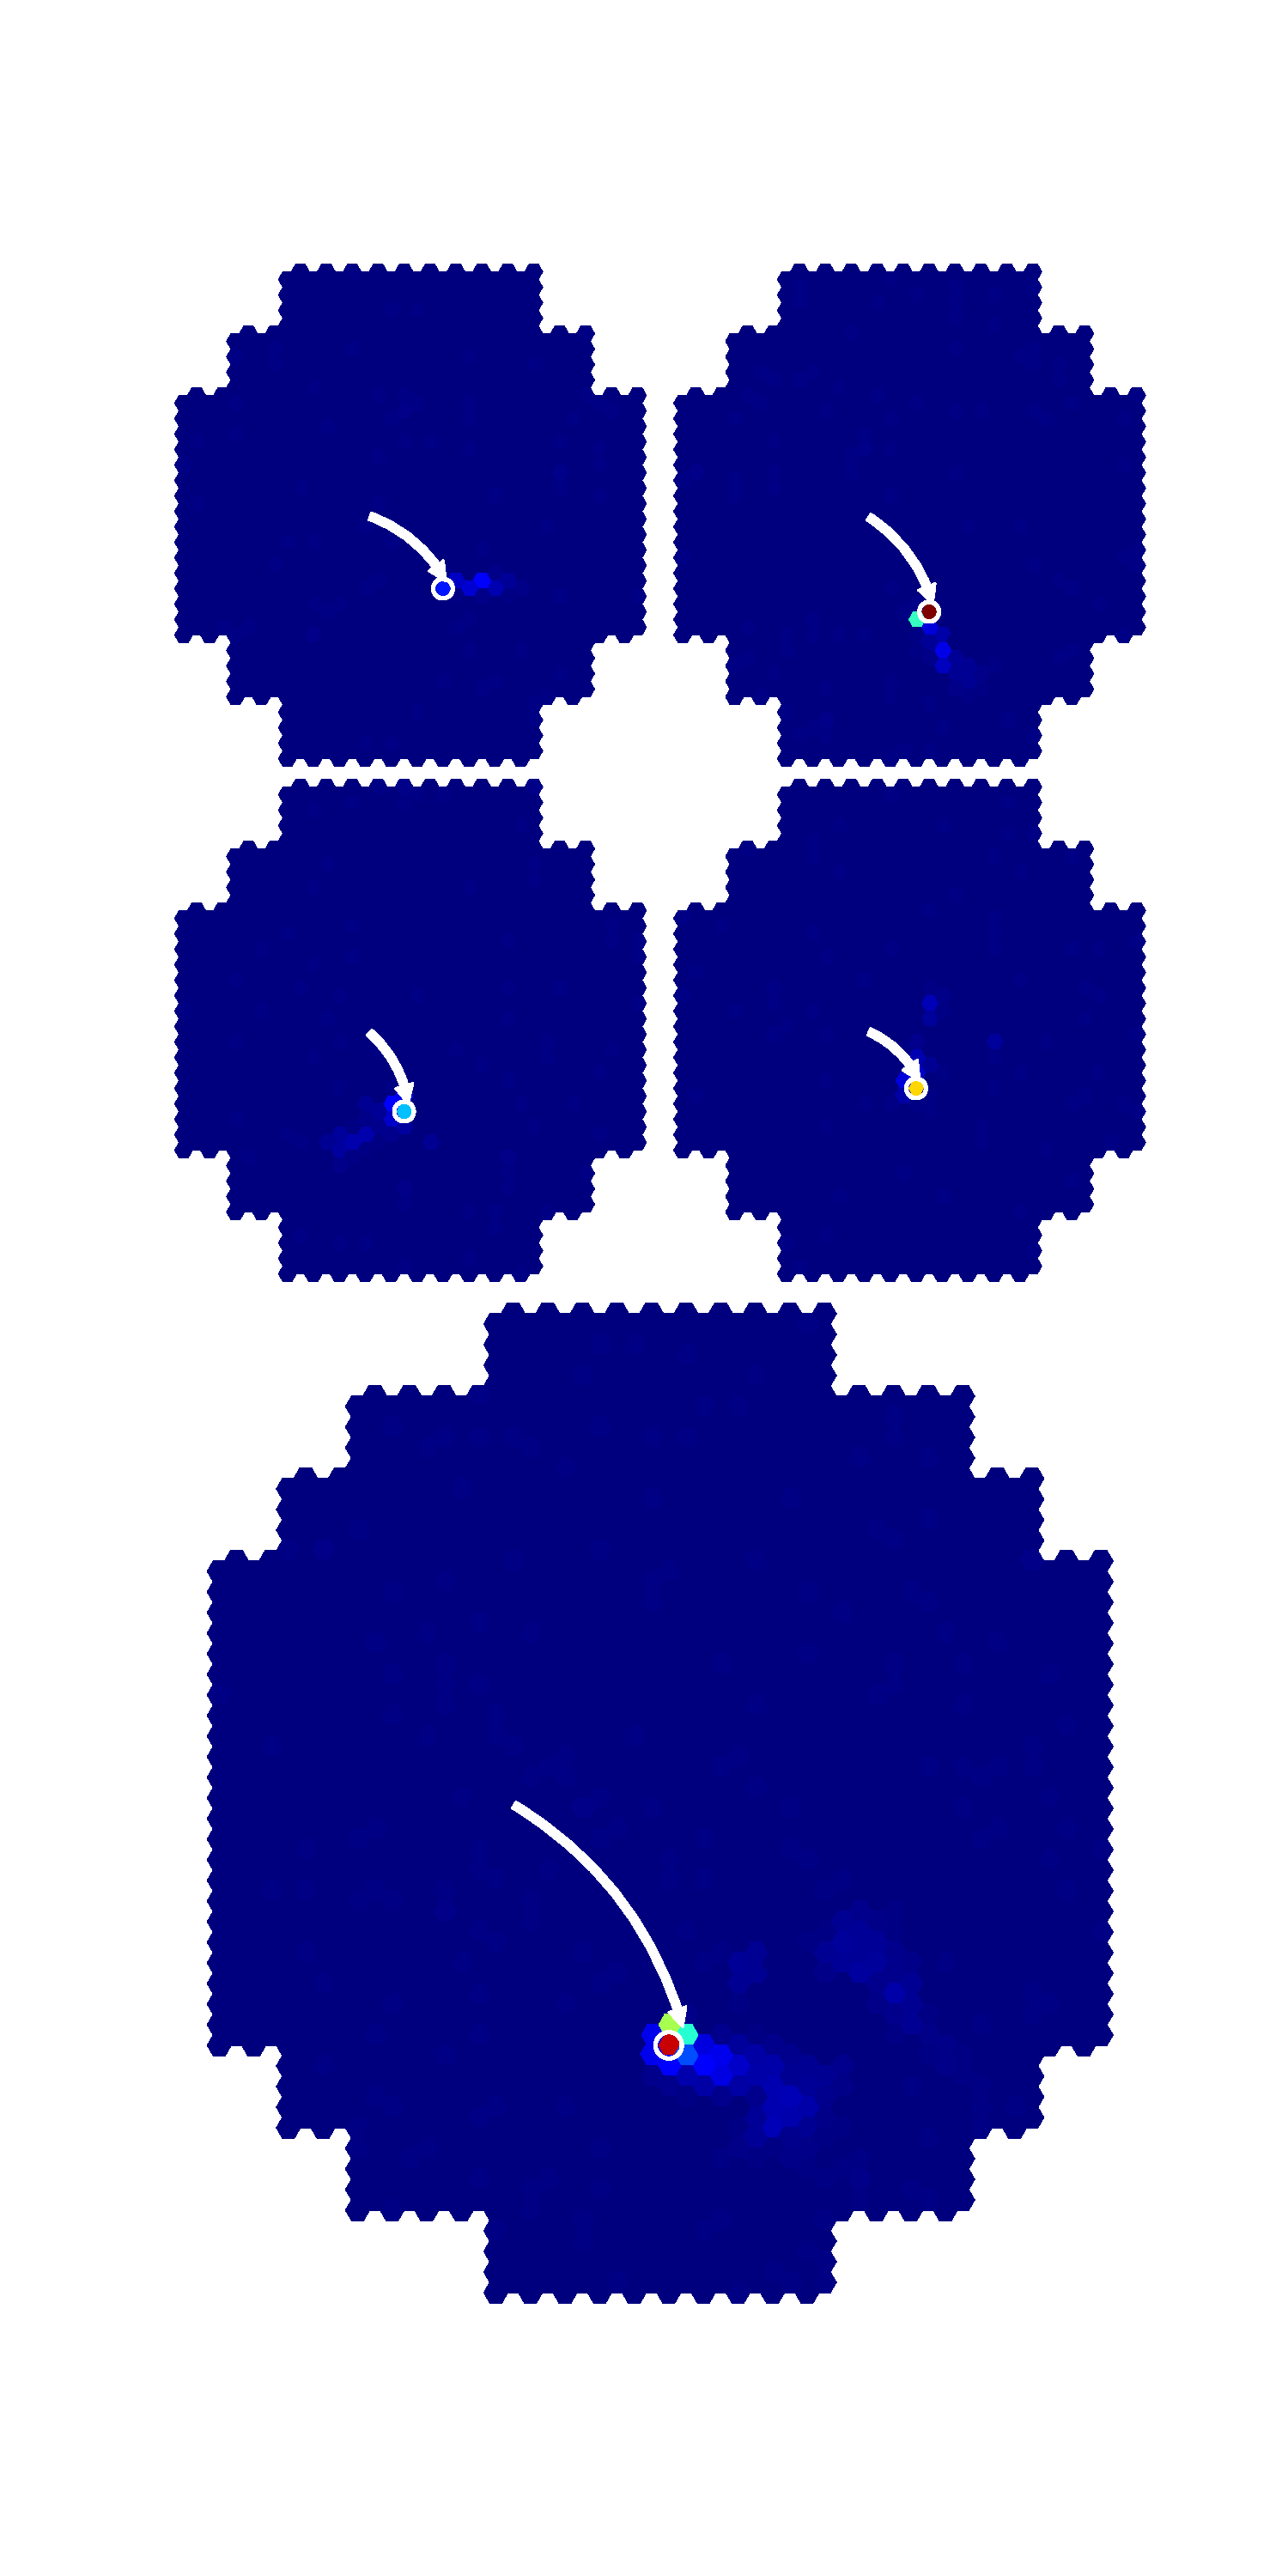
\includegraphics[trim=80 120 80 150,clip,width=\textwidth]{graphDC}
\caption{A typical camera image without the EAS shower. The DC light is visible in every telescope, indicated by the white arrow. The DC pixel is circled in white. The largest telescope image is from CT5, but was not used in analysis.}
\label{fig:DCtelimage}
\end{minipage}\hfill
\begin{minipage}{0.45\textwidth}
\centering
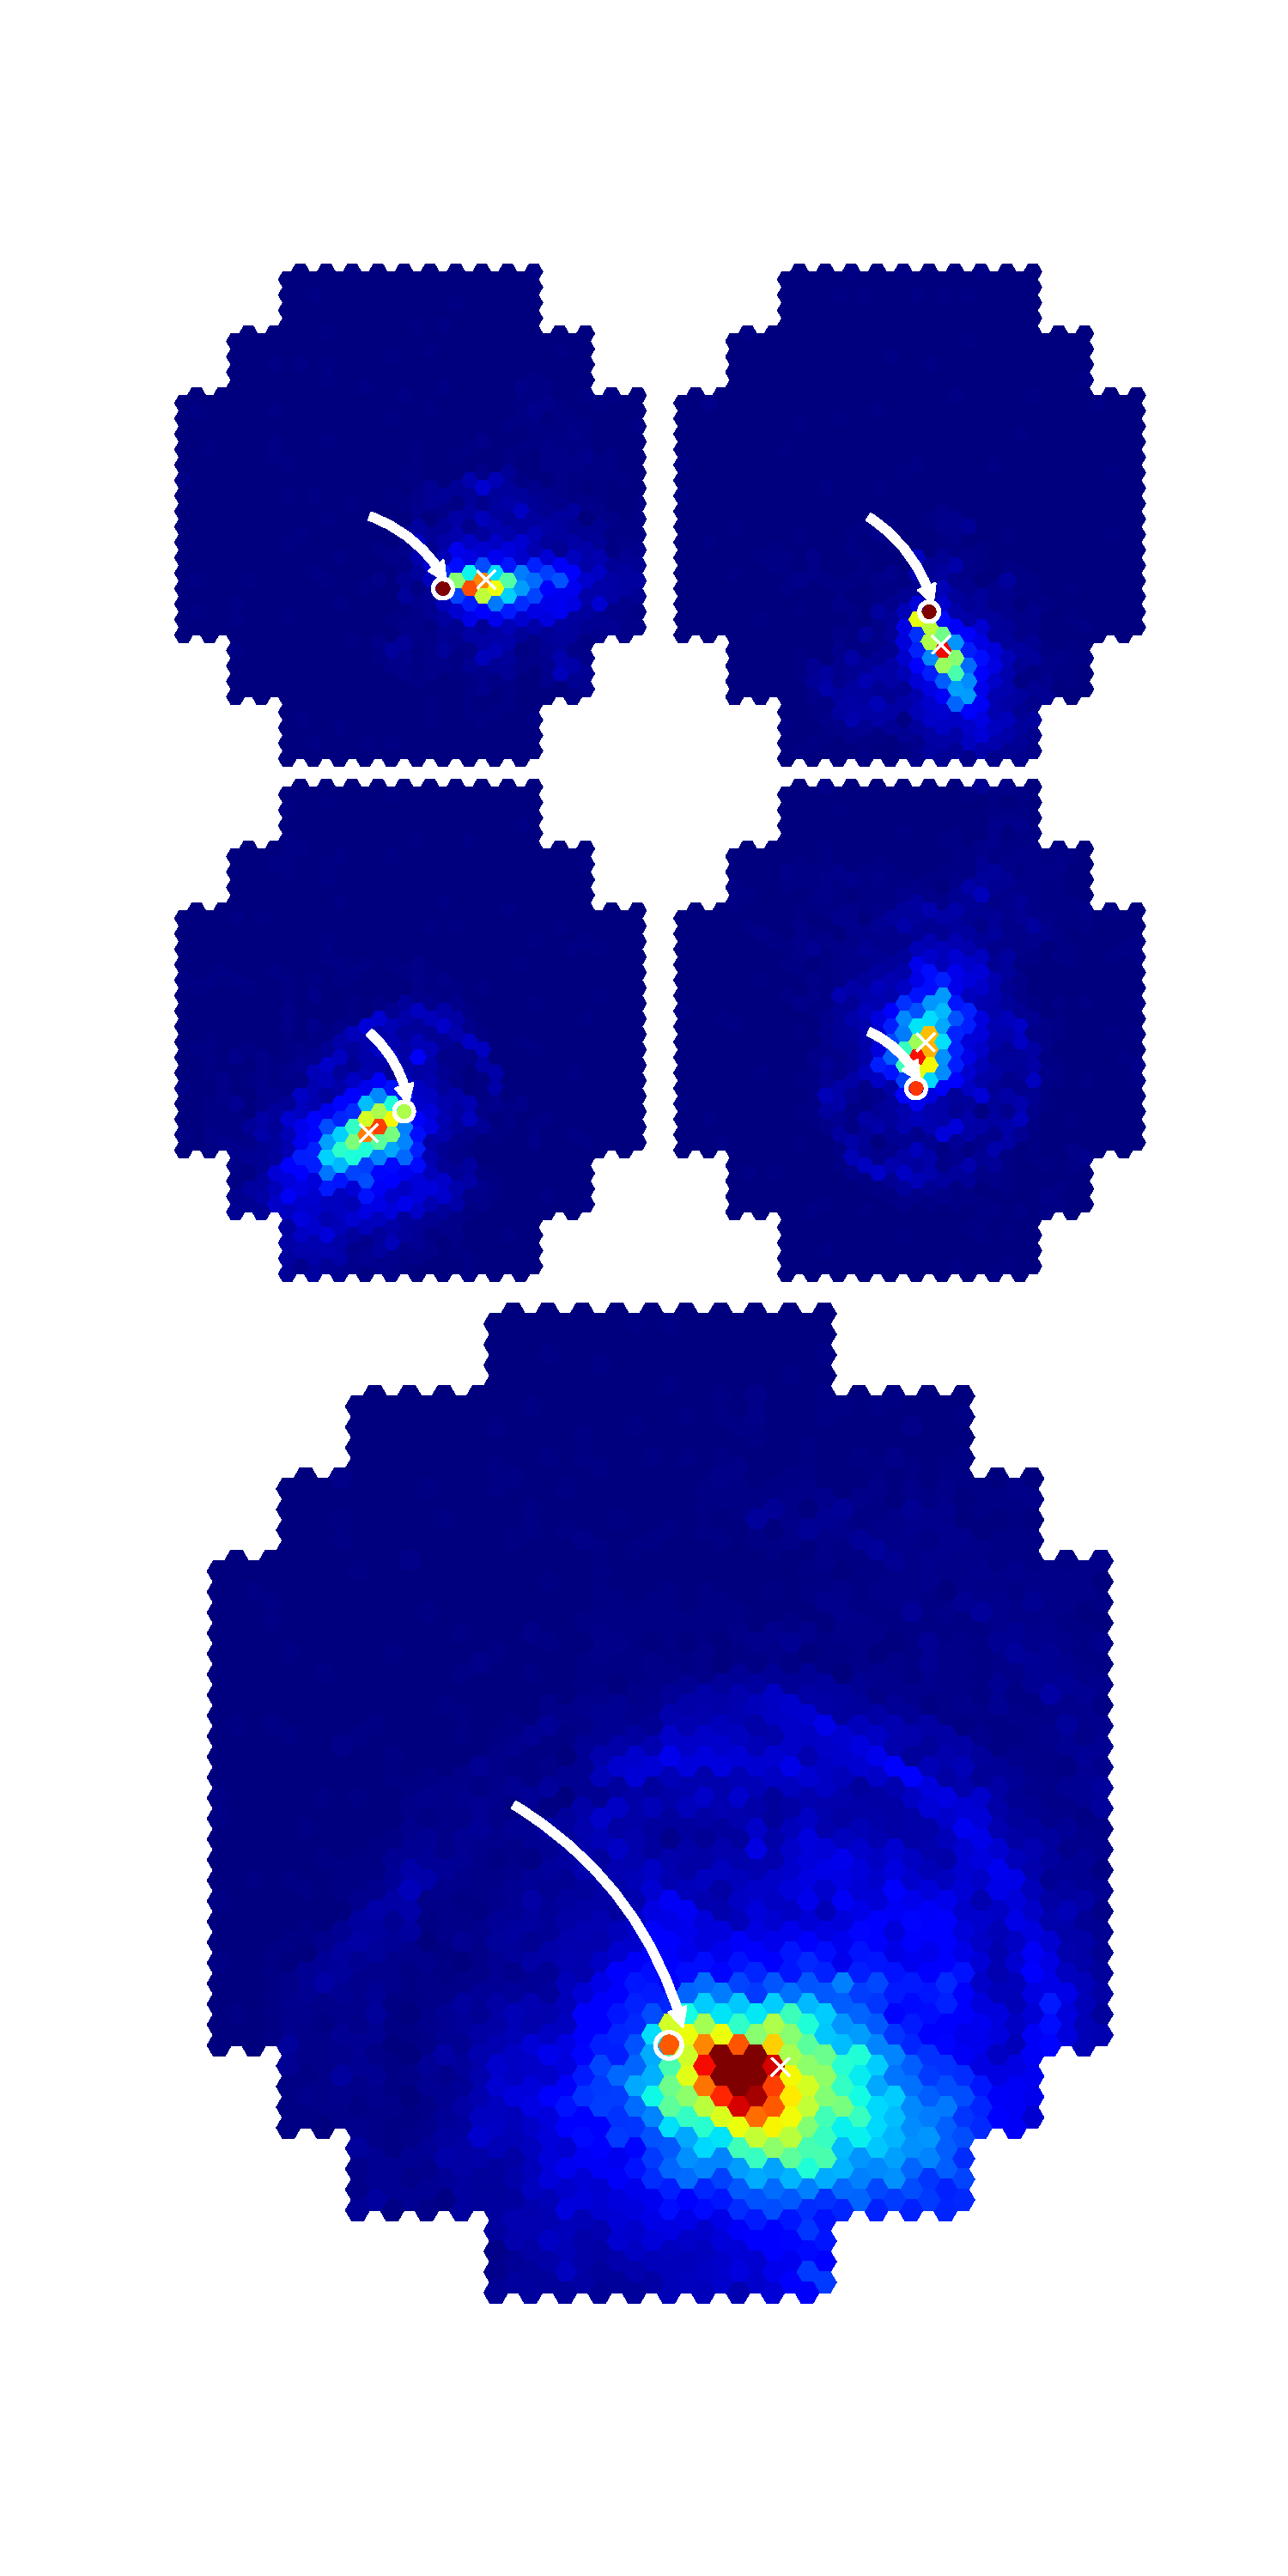
\includegraphics[trim=80 120 80 150,clip,width=\textwidth]{graphfull}
\caption{The same shower as in \ref{fig:DCtelimage} is shown here with the inclusion of the EAS shower. The DC light is pixels indicated with a white arrow and circle. The shower center of gravity is marked by a white cross.}
\label{fig:cutdistribution2}
\end{minipage}
\restoregeometry
\end{figure}

The various pixel entry variables were found from the sim\textunderscore telarray output. The HESS telescope pixels have a high gain Channel 0 and a low gain Channel 1, with both voltages undergoing a Flash Analogue-to-Digital Conversion (FADC). The simulated value of the FADC Voltage for each channel was found. Using the pedestal and gain, the quantity $Intensity = (FADC - Pedestal)\times Gain $ was calculated for each channel. Due to possible saturation of the high gain FADC, only the low gain $Intensity$ was used. Sim\textunderscore telarray also derives various Hillas whole-image parameters. These include the image width and length measured in degrees, from which the aspect ratio $A.R = \frac{width}{length}$ was calculated. The reconstructed shower direction and the shower center of gravity were also calculated, as positions in azimuth and zenith. Additionally the estimated energy and distance from each telescope to core, $r_{core}$,  were found.

For every pixel, in addition to the $Intensity$, its location within the telescope image was determined using the standard HESS layout. The variables $ \Delta_{C.o.G}$, $\Delta_{Direction}$ and $\Delta_{Line}$ were defined as the distance from the pixel to the shower center of gravity, shower direction, and the line joining those two points. Furthermore, the nearest neigbouring pixel IDs were calculated for every pixel position, enabling the $Intensity$ in each neighbouring pixel to be found. The largest neighbouring intensity was identified, and the ratio $Q_{DC} = \frac{Intensity_{N.N.max}}{Intensity}$ was derived. Similarly the largest neighbouring FADC was found, and the ratio $raw_{Q} = \frac{FADC_{N.N.max}}{FADC}$ was calculated. In addition, the Nearest Neighbour Mean Intensity $Mean_{N.N}$ was recorded, as well as the smallest neighbouring pixel intensity $Intensity_{N.N.min}$. The variable $DC_{Signal} = Intensity-Mean_{N.N}$ was defined as an rough guess of the \textquoteleft DC signal' component in the pixel. Lastly the Image Amplitude $I_{tot}$, defined as the total image intensity after the default tail cuts have been applied to the image.

\subsection{Classic HESS1 DC Pixel Identification}
As a basis for comparison, the original HESS cuts listed in Table \ref{tab:table1} were replicated for the set of test data. For every HESS1 image, the total image amplitude $I_{tot}$ was used alongside the zenith angle $\theta$ to determine a dynamic cut, $Q_{DC} < 0.14 \times \log(\frac{I_{tot}}{161 \times \cos \theta})$. Among those pixels passing all cuts, the one with the smallest $Q_{DC}$ was selected as the DC pixel candidate for the image. Because many images had no pixel that passed all cuts, the $Q_{DC}$ method was frequently unable to identify a DC pixel. In the original analysis, an additional cut $r_{core} \textgreater 40m$ was applied. However, the uncertainty in determining the core position through Hillas Analysis is typically of the order of $\pm 30m$. Consequently, this particular cut was omitted.

\begin{table}[h!]
  \centering
  \caption{Cuts applied to image pixel sets, used by HESS collaboration \cite{hess07}}
  \label{tab:table1}
  \begin{tabular}{ccc}
    \toprule
    Variable & Cut\\
    \midrule
     $ \Delta_{C.o.G}$ & \textgreater 0.17 \\
     $ \Delta_{C.o.G}$ & \textless 0.91 \\
     $\Delta_{Direction}$ & \textless 0.45 \\
     $\Delta_{Line}$ & \textless 0.23 \\
     Aspect Ratio & \textless 0.75 \\
     $Q_{DC}$ & \textless 0.14$ \times \log(\frac{I_{tot}}{161 \times \cos \theta})$ \\
    \bottomrule
  \end{tabular}
\end{table}

The candidates were checked against the true DC pixels identified in the EAS-free images. From the testing sample, 1.81\% of all HESS1 images were correctly identified and passed the cuts. Once misidentified events were considered, the post-cuts sample was 77.8\% accurate, as shown in Figure \ref{fig:cutdistribution}. These values will serve as a useful benchmark for BDT performance. Increasing the acceptance rate will be essential for enabling spectroscopic analysis of cosmic rays, by providing more events to analyse.

\begin{figure}
\begin{center}
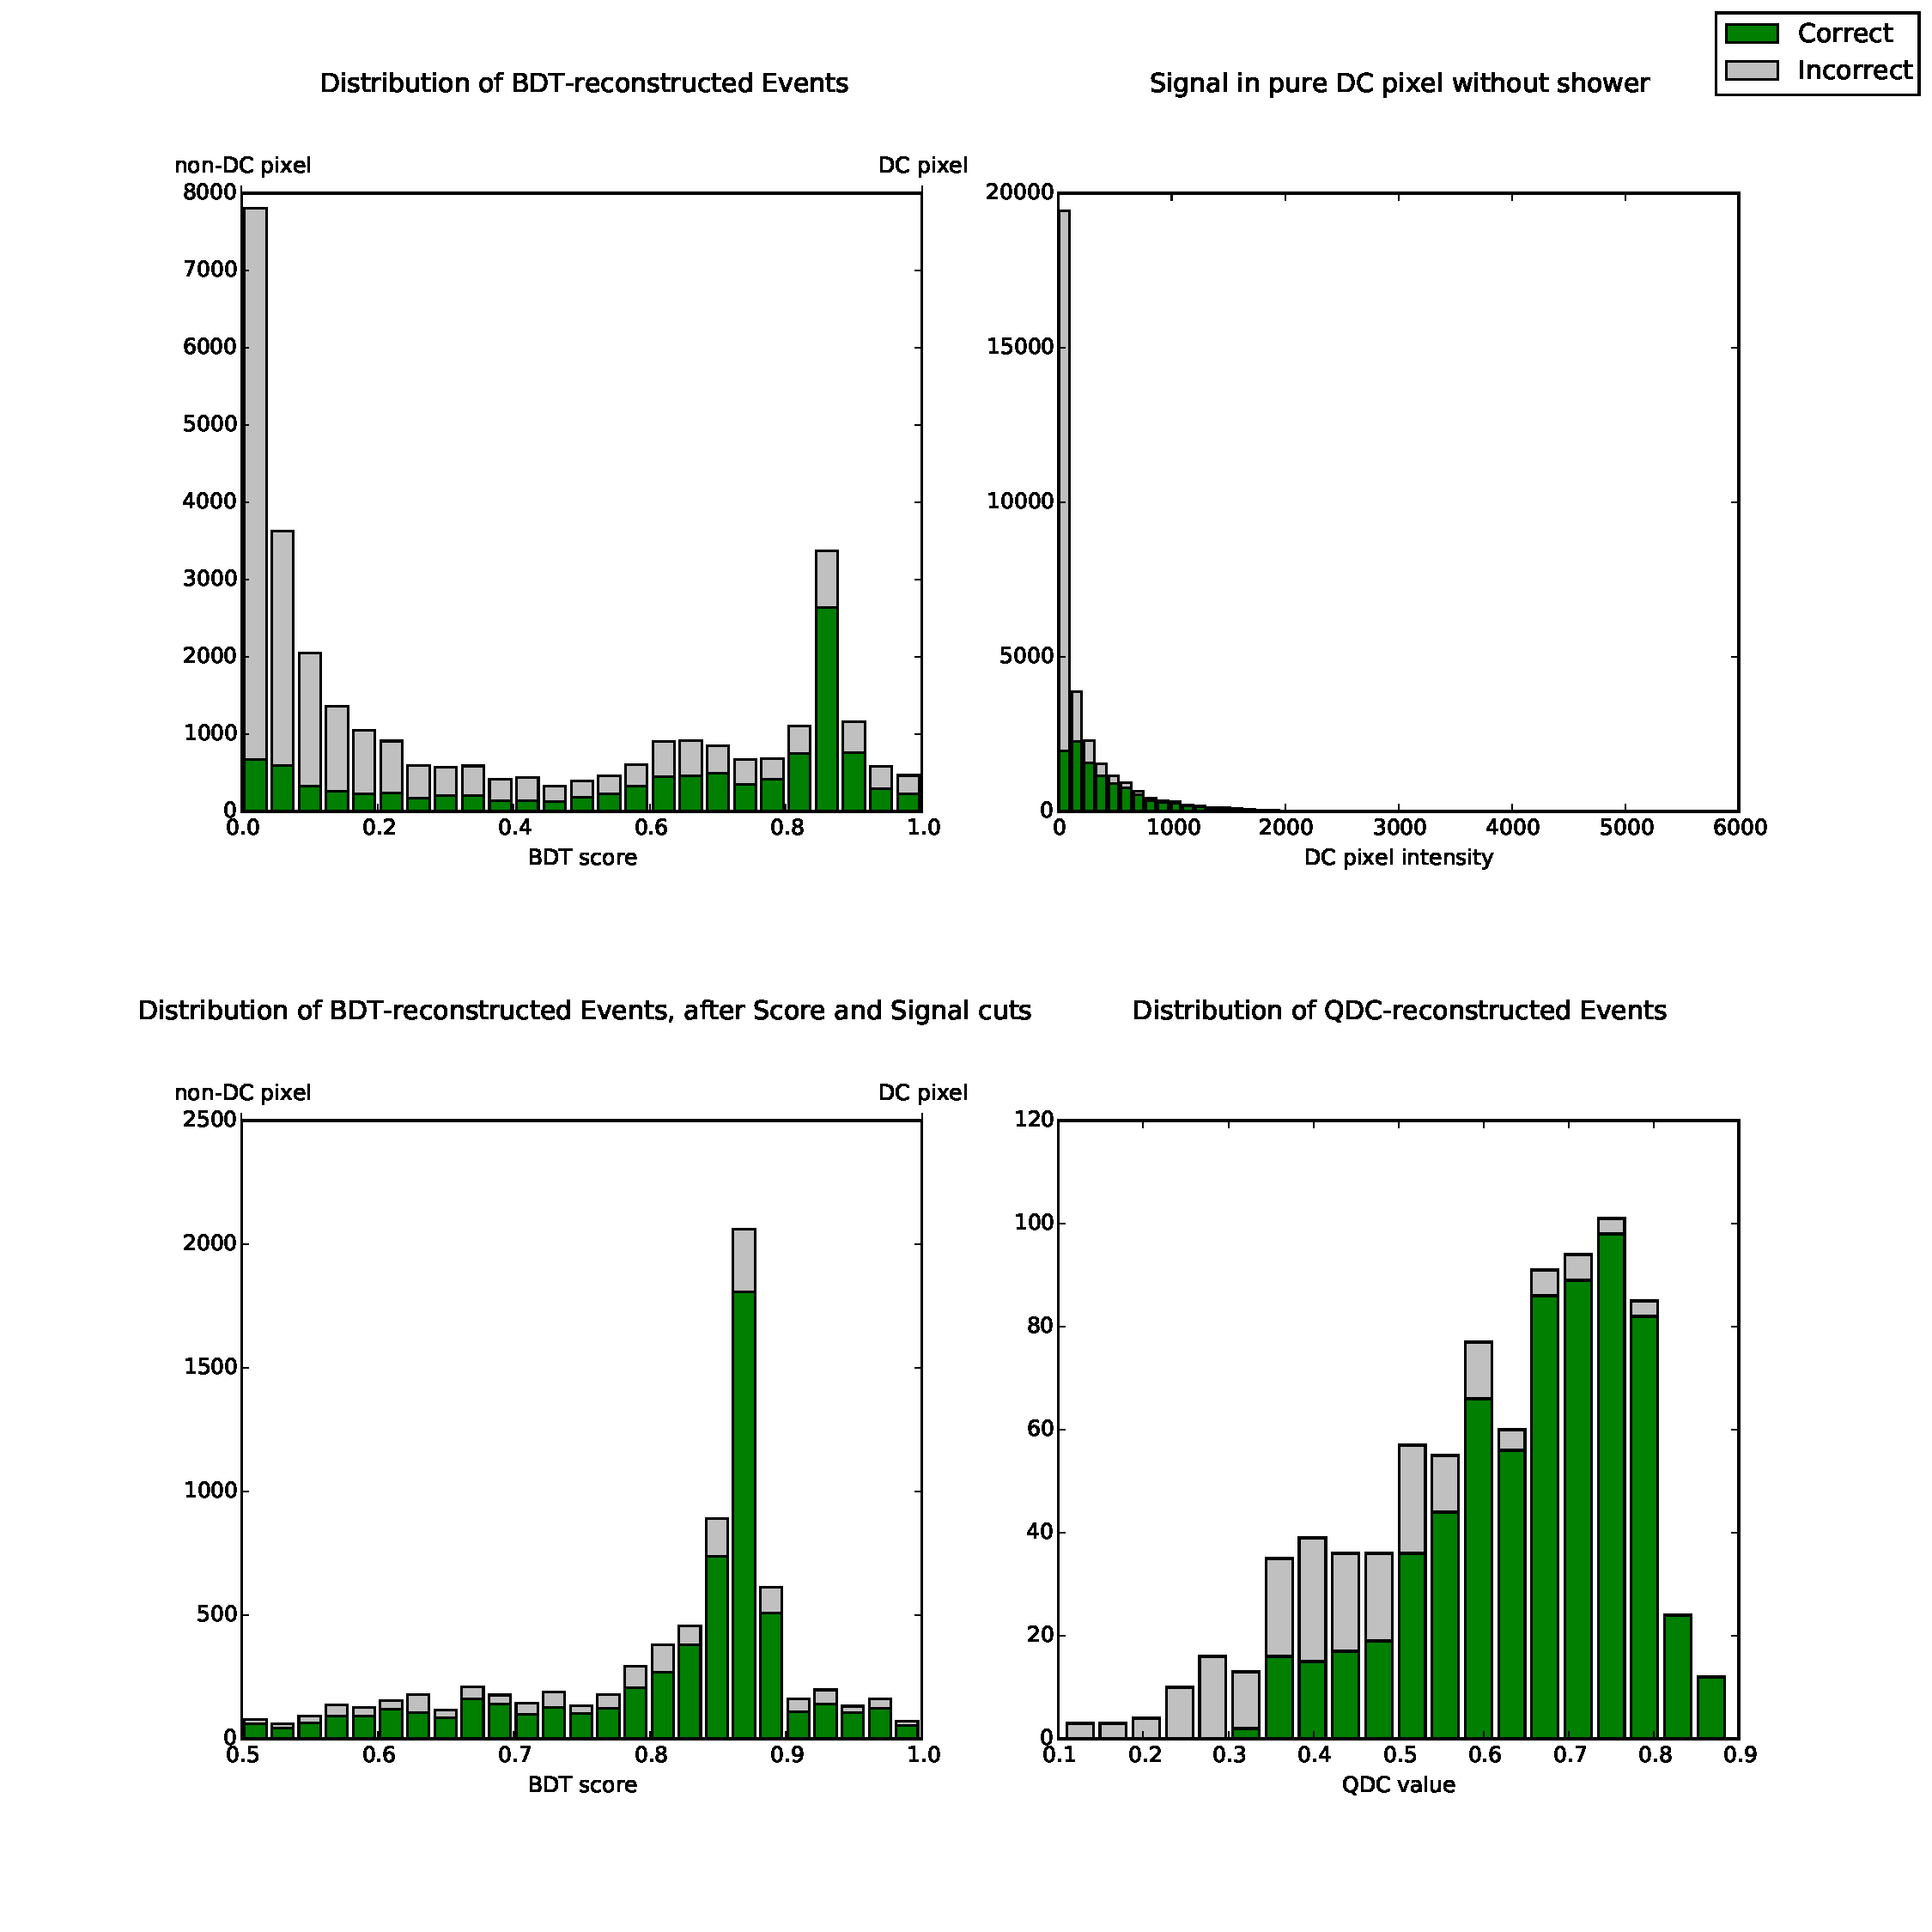
\includegraphics[width=\textwidth]{hess1statsbigtestdata}
\caption{The DC signal in the shower-free pixel is shown in the top left, with a broad gaussian distribution with the tail of the night-sky background extending up to appproximately 5000. Events below this are unlikely to be identified correctly because the DEC light is too faint. In the top right- the distribution of the dataset is shown, once all the non-$Q_{DC}$ cuts have been applied. In the bottom left, the BDT score distribution is shown before any cuts. On the bottom right, we see the same distribution after both signal and BDT score cuts are applied. All green events are ones in which the DC pixel has been correctly identified, while red events are ones that have been incorrectly identified.}
\label{fig:cutdistribution}
\end{center}
\end{figure}

\subsection{Boosted Decision Tree DC Identification}
As an alternative to use of $Q_{DC}$, a new method of DC pixel identification was developed as part of this analysis by using a BDT trained with the Scikit Learn Python package \cite{scikit-learn}. Using the training set of 2000 CORSIKA events, and randomly split further, with 90\% in a learning subset and 10\% in a subset to check for overtraining. Within the learning subset, every HESS 1 image was used, provided it was triggered in both EAS-free and full-shower simulations. For each of the triggered image pixels, an entry was formed with the variables listed in table \ref{tab:hess1classifier}. A class of 0 was assigned to every non-DC pixel, and a class of 1 was assigned to every DC pixel. Having created a dataset, the BDT was then trained with a maximum depth of 8, and with 100 trees generated. The data was provided in the form of individual pixel entries, rather than as discrete sets for images or events.

\begin{table}[h!]
  \centering
  \caption{Relative Feature Importance in HESS-1 BDT training}
  \label{tab:hess1classifier}
  \begin{tabular}{ccc}
    \toprule
    Variable & Relative Importance\\
    \midrule
    $DC_{Count}$ & 0.33\\
    $Mean_{N.N}$ & 0.24\\
    $Q_{DC}$ & 0.14\\
    $\Delta_{Direction}$ & 0.12\\
    Image Amplitude & 0.07\\
    $raw_{Q}$ & 0.05\\
    $\Delta_{Line}$ & 0.02\\
    $Intensity$ & 0.02\\
    \bottomrule
  \end{tabular}
\end{table}

The relative importance of each \textquoteleft feature' is automatically calculated by the Scikit Learn package, and is also recorded in table \ref{tab:hess1classifier}. The variable $DC_{Count}$ was consistently the most importance variable across many combinations of included variables and BDT training parameters. It was found that, under the conditions listed above, the BDT was 99.94 \% accurate for the learning pixel subset, and 99.94 \%  accurate for the overtraining-check pixel subset. This indicates that the BDT was not significantly overtrained, which would otherwise be manifested by a large divergence in accuracy between learning and overtraining-check data.

Having trained the BDT successfully, it was then applied to the same test dataset as for the classic $Q_{DC}$ identification. In each camera image, the event with the largest BDT score was deemed to be \textquoteleft most signal-like', and thus selected as the DC pixel candidate. A cut was applied, requiring $P_{signal} > 0.5$ for the DC candidate to be accepted. A second cut requiring $DC_{Count} > 150$ removed many incorrectly identified events. Application of this combined cut greatly increases the successful identification rate. From the testing sample, 16.01\% of all images were correctly identified and passed the cuts. The BDT was found to be 79.2\% accurate in identifying DC pixels which passed the cuts. This represents a very significant improvement in pixel identification efficiency, as well as a minor increase in accuracy after cuts. 

The results are summarised in Table \ref{tab:qdcbdtcomparison1}. The BDT method represents a clear improvement in DC pixel identification over the previous $Q_{DC}$ method, and corresponds to a fifteen-fold increase in identified pixels. 

\begin{table}[h!]
  \centering
  \caption{Comparison of $Q_{DC}$ and HESS 1 BDT Performance}
  \label{tab:qdcbdtcomparison1}
  \begin{tabular}{ccc}
    \toprule
    & $Q_{DC}$ & BDT\\
    \midrule
    Pixels Accepted and Correctly Identified (\%)  & 1.81 & 16.01\\
   Pixels Accepted and Incorrectly Identified (\%)  & 0.52& 4.22\\
    Sample Purity (\%)  & 77.8 & 79.2 \\
    \bottomrule
  \end{tabular}
\end{table}

\subsection{HESS-2 BDT}
The original HESS study predated the construction of the larger CT5 telescope, and thus focused exclusively in the four HESS-1 telescopes. Although the cuts in \ref{tab:qdccuts} were not optimised for the differing pixel size and angular viewing region of CT5, they were replicated to provide a basis for comparison. Based on CT5 images from the training sample, an increased 5.6\% of DC pixels were correctly identified and passed the required cut. A further 11.3 \% of all pixels passed the cuts, despite being misidentified. This represented a very heavy decrease in sample purity to just 33.0\%. We can assume that better optimised CT5 cuts could remove many of these misidentified events, though it is unlikely that any significant improvement in the number of correctly identified DC pixels would be possible. Thus, the number of DC pixels successfully identified using the $Q_{DC}$ method is still a valid benchmark for comparative BDT performance. A true accuracy rate closer to the HESS 1 rate of 90\% could be expected. Due to the distinctiveness of the CT5 telescope, direct application of the HESS1 classifier to the CT5 telescope yields poorer BDT performance. To improve CT5 pixel identification, a separate HESS2 BDT was instead trained with the same variables as above. The relative feature importance is listed in Table \ref{tab:hess2classifier}. 

\begin{table}[h!]
  \centering
  \caption{Relative Feature Importance in HESS-2 Classifier BDT training}
  \label{tab:hess2classifier}
  \begin{tabular}{ccc}
    \toprule
    Variable & Relative Importance\\
    \midrule
    $DC_{Count}$ & 0.32\\
    $Mean_{N.N}$ & 0.24\\
    $raw_{Q}$ & 0.09\\
    $Q_{DC}$ & 0.08\\
    $\Delta_{Direction}$ & 0.8\\
    Image Amplitude & 0.07\\
    $Intensity$ & 0.06\\
    $\Delta_{Line}$ & 0.04\\
    \bottomrule
  \end{tabular}
\end{table}

For the training events, the classifier was 99.97\% accurate, while for the overtraining check data, it was 99.96\% accurate. The classifier was thus not significantly overtrained. Applying the new classifier lede to an improvement in CT5 classification, with 17.9 \% of pixels being correctly identified and accepted, and an accuracy of 66.1\%. Despite this improvement, a clear gap emerged between the between the performance of HESS1 classifier on old telescopes, and the performance of the HESS2 classifier on CT5. Part of this discrepancy can be explained by the HESS2 learning dataset, which has just one DC pixel per event rather than the four HESS1 DC pixels. Additionally, HESS 2 images will have roughly 2600 non-DC pixels per event, versus 3600 DC pixels per event for HESS 1 images. The HESS2 classifier was thus trained on significantly fewer DC pixels, so we would expect to see the clear performance gap in comparison to the HESS1 classifier.  

\begin{table}[h!]
  \centering
  \caption{Comparison of $Q_{DC}$ and HESS 2 BDT Performance}
  \label{tab:qdcbdtcomparison2}
  \begin{tabular}{ccc}
    \toprule
    & $Q_{DC}$ & BDT\\
    \midrule
    Pixels Accepted and Correctly Identified (\%) & 5.59 & 18.52 \\
   Pixels Accepted and Incorrectly Identified (\%) & 14.75 & 4.44 \\
    Sample Purity (\%) & 27.5 & 80.6 \\
    \bottomrule
  \end{tabular}
\end{table}

\subsection{High Multiplicity Events}
For LPD event reconstruction, we require at least four measurements of the DC light. We define the telescope multiplicity of an event as the number of DC pixels which are identified and pass all cuts. Telescope multiplicity measures both HESS1 and HESS2 pixels. A \textquoteleft high-multiplicity event' is one in which we have telescope multiplicity $>3$. If we only consider high-multiplicity events, we can determine the $Q_{DC}$ performance for use in LPD reconstruction. After applying this cut, there were was just one single high-multiplicity event found using the $Q_{DC}$ method. This meant that just 0.01\% of all pixels were accepted, although with a sample purity of 100\%. Because the final sample consisted of just three HESS1 pixels, and one HESS2 pixel, the associated Poissonian error in acceptance rates and accuracy rates will be extremely large.

Through we application of the two HESS classifiers, we can find the comparative high-multiplicity BDT performance. If we only consider high-multiplicity BDT events, the fraction of correctly identified HESS1 DC pixels falls to 2.2\%, while the fraction of incorrectly identified pixels passing the cuts falls to 0.2\%. The sample purity increases slightly to 91.2\%. In the case of the high-multiplicity HESS2 images, the BDT performance gap narrows somewhat. In total 1.9\% of pixels are correctly identified and accepted, although the accuracy rate is only increased to 80.7\%. The relatively high fraction of passing events is in excess of the random expectation of $0.16^{4}=0.07\%$ and $0.19^{4}=0.13\%$ for HESS1 and HESS2. This suggests that DC pixel identification between different telescope images is strongly correlated. The same is true for the $Q_{DC}$ high multiplicity rates. As well as general BDT accuracy improving after high-multiplicity cuts, the performance gap over the $Q_{DC}$ method is vastly increased for high-multiplicity events. As a result of the two-hundred-fold increase in acceptance rate for high multiplicity events, the expected data sample size will increase dramatically. This should enable spectroscopic analysis of Cosmic Ray Elements to be conducted after a much shorter experimental run time that for the $Q_{DC}$ method.

\begin{table}[h!]
  \centering
  \caption{Comparison of high-multiplicity performance Performance}
  \label{tab:highmultiplicitycomparison}
  \begin{tabular}{c|cc|cc}
    \toprule
    & \multicolumn{2}{c|}{HESS 1} & \multicolumn{2}{c}{HESS 2} \\
    & $Q_{DC}$ & BDT & $Q_{DC}$ & BDT\\
    \midrule
    High Multiplicity Pixels Accepted and Correctly Identified (\%)& 0.01 & 2.20 & 0.01 & 1.61\\
    High Multiplicity Pixels Accepted and Incorrectly Identified (\%)  & 0.00 & 0.43 & 0.01 & 0.22\\
    Sample Purity (\%)& 100.0 & 83.8 & 100.0 & 88.0\\
    \bottomrule
  \end{tabular}
\end{table}

\subsection{Proton Background}
It is important to discriminate between the heavy cosmic ray elements, such as iron, and the much more abundant proton events. Protons tend to emit negligible DC light, so will contaminate any data sample with events that cannot be reconstructed using the LPD method. To determine the acceptance rate for proton events, a simulation was conducted with 5000 proton events in CORSIKA. For HESS1, the raw acceptance rate was 15.1\% while the sample purity of 32.2\%. For HESS2, the raw acceptance rate was 58.6\% while the sample purity of 6.8\%. Although the HESS1 acceptance rate is relatively small, the proton flux is approximately ten times greater than iron flux. A mixed sample would have many more proton images than iron images. Once multiplicity cuts are applied, the acceptance rate falls steeply to just 2.9\%. With the factor 10 discrepancy in flux, the number of proton and iron images will be comparable. Of those passing the cuts, 24.5\% are correctly identified.  For HESS2, the comparable number is 21.7\% with multiplicity cuts. The sample purities are just 24.4\% and 7.7\% respectively. This poor performance motivates our desire to remove protons from our sample for analysis.

We require an additional cut to remove the majority of these proton events. If we can eliminate one or two accepted proton images per event, then the remaining proton pixels will all be rejected by the multiplicity cuts. Hence, loose cuts can sharply reduce the acceptance rate of protons. In this case, as shown in Figure \ref{fig:aspectratio}, there is a fair degree of separation between proton and Iron Aspect Ratio for pixels which pass all cuts. We aim to remove proton pixels but not iron pixels. Applying a cut requiring Aspect Ratio $> 0.35$ eliminated all accepted proton events for HESS1 and HESS2. With 17792 total HESS1 images, just 6195 images were triggered by DC light. Of all 17792 images, there were none passing all of the required cuts. We can place a poissonian upper limit on the acceptance rate of $< 0.02 \%$. Of the for 4448 HESS2 images, just 2169 contained DC light. As no image passed all cuts, we place an upper limit of $< 0.07\%$. 

Using poissonian statistics, we can place a 95\% confidence upper limit on the rate of accepted, high-multiplicity $Q_{DC}$ events. By virtue of passing a multiplicity cut, the number of accepted pixels must be at least 4, or none. It is thus more appropriate to instead consider the total number of events for calculations of an upper limit. There were 4711 fully triggered events, of which none were \textquoteleft High multiplicity Events'. We find a value for the mean $\lambda$ such that the probability of not observing a high multiplicity event is less than 5\%.
\[ P(n|\lambda)=\frac{e^{-\lambda}\lambda^{n}}{n!} \Longrightarrow P(0|\lambda)=\frac{e^{-\lambda}\lambda^{0}}{0!}=e^{-\lambda}=0.05
\Longrightarrow
\lambda = -\ln(0.05)=3.00\]

Thus, we can conclude that if the mean was greater that if the mean $\lambda>3$, we would have expected to observe at least one event with a 95\% probability. As we did not observe an event, we conclude that the mean high multiplicity event rate is less than $\frac{3}{4711}=0.06\%$. 

For HESS1 iron events, the total acceptance rate falls slightly from 2.4\% to 2.3\%, while the sample purity decreases slightly to 89.0\%. For HESS2, the total acceptance rate falls slightly from 2.4\% to 2.3 \%, while the sample purity decreases slightly to 79.8\%. Iron images form at least 75\% of a sample, because most proton images are at least one hundred times less likely to be accepted. Use of this BDT method is thus assumed throughout the rest of this analysis.

\begin{figure}
\begin{center}
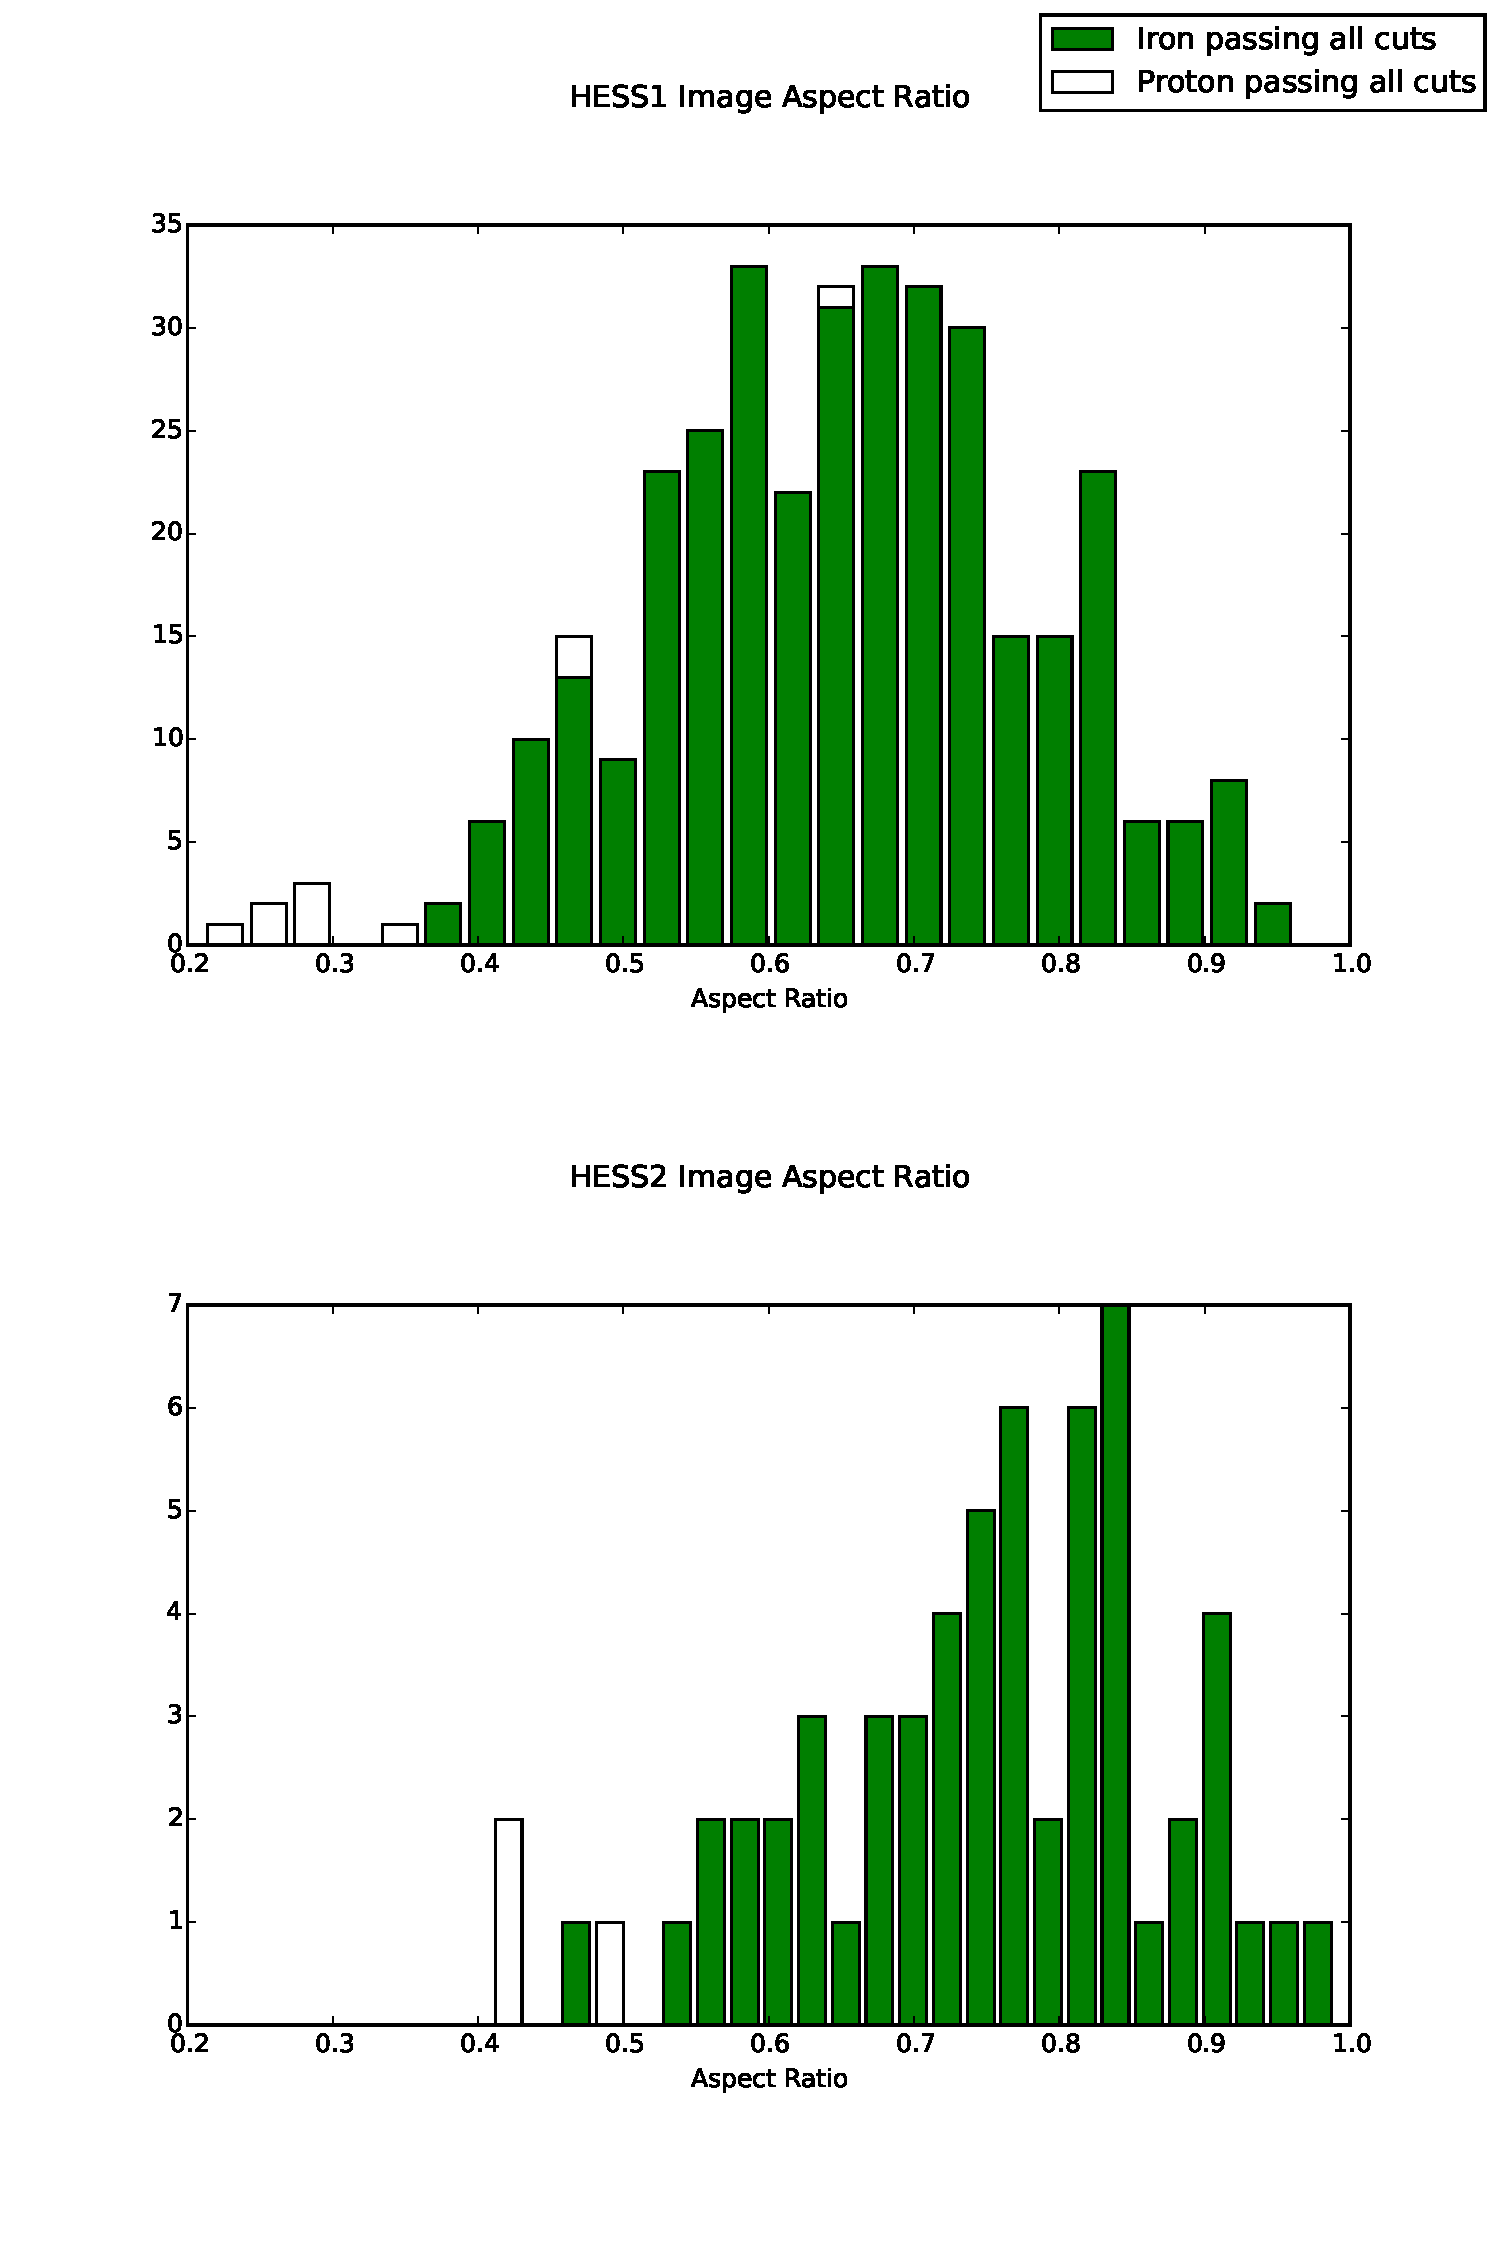
\includegraphics[width=0.9\textwidth]{aspectratio}
\caption{The aspect ratio of images in events which pass the multiplicity cut are shown. It is clear that the proton events have a strong tendency towards lower Aspect Ratios. We must remove the white proton pixels passing all other cuts, without removing dark green iron pixels passing all other cuts. A cut requiring Aspect Ratio $> 0.35$ should remove a large proportion of proton images without reducing the pass rate for iron nucleii.}
\label{fig:aspectratio}
\end{center}
\end{figure}

\begin{table}[h!]
  \centering
  \caption{Comparison of Proton and Iron Acceptance}
  \label{tab:protonacceptance}
  \begin{tabular}{ccc}
    \toprule
    & HESS1  & HESS2 \\
    \midrule
    Proton Pixels Accepted (\%) & 15.10 & 32.68\\
    Sample Purity (\%) & 10.1 & 5.1 \\
    \midrule
    High Multiplicity Proton Pixels Accepted (\%) & 0.83 & 1.03\\
    Sample Purity (\%) & 6.8 & 4.3 \\
    \midrule
    Proton Pixels Accepted after All Cuts(\%) & $< 0.06$ & $< 0.06$\\
    Sample Purity (\%) & / & / \\
    \midrule
    Iron Pixels Accepted after All Cuts(\%) & 2.44 & 1.66\\
    Sample Purity (\%) & 84.3 & 88.2 \\
    \bottomrule
  \end{tabular}
\end{table}

\section{HESS-type Event Simulation}

\subsection{Extended Air Shower Background}
Having successfully parameterised the LPD using CORSIKA simulations, we can replicate it for out Monte Carlo simulation. We have found that the DC LPD is broadly independent of both height and Energy. 


\begin{figure}
\begin{center}
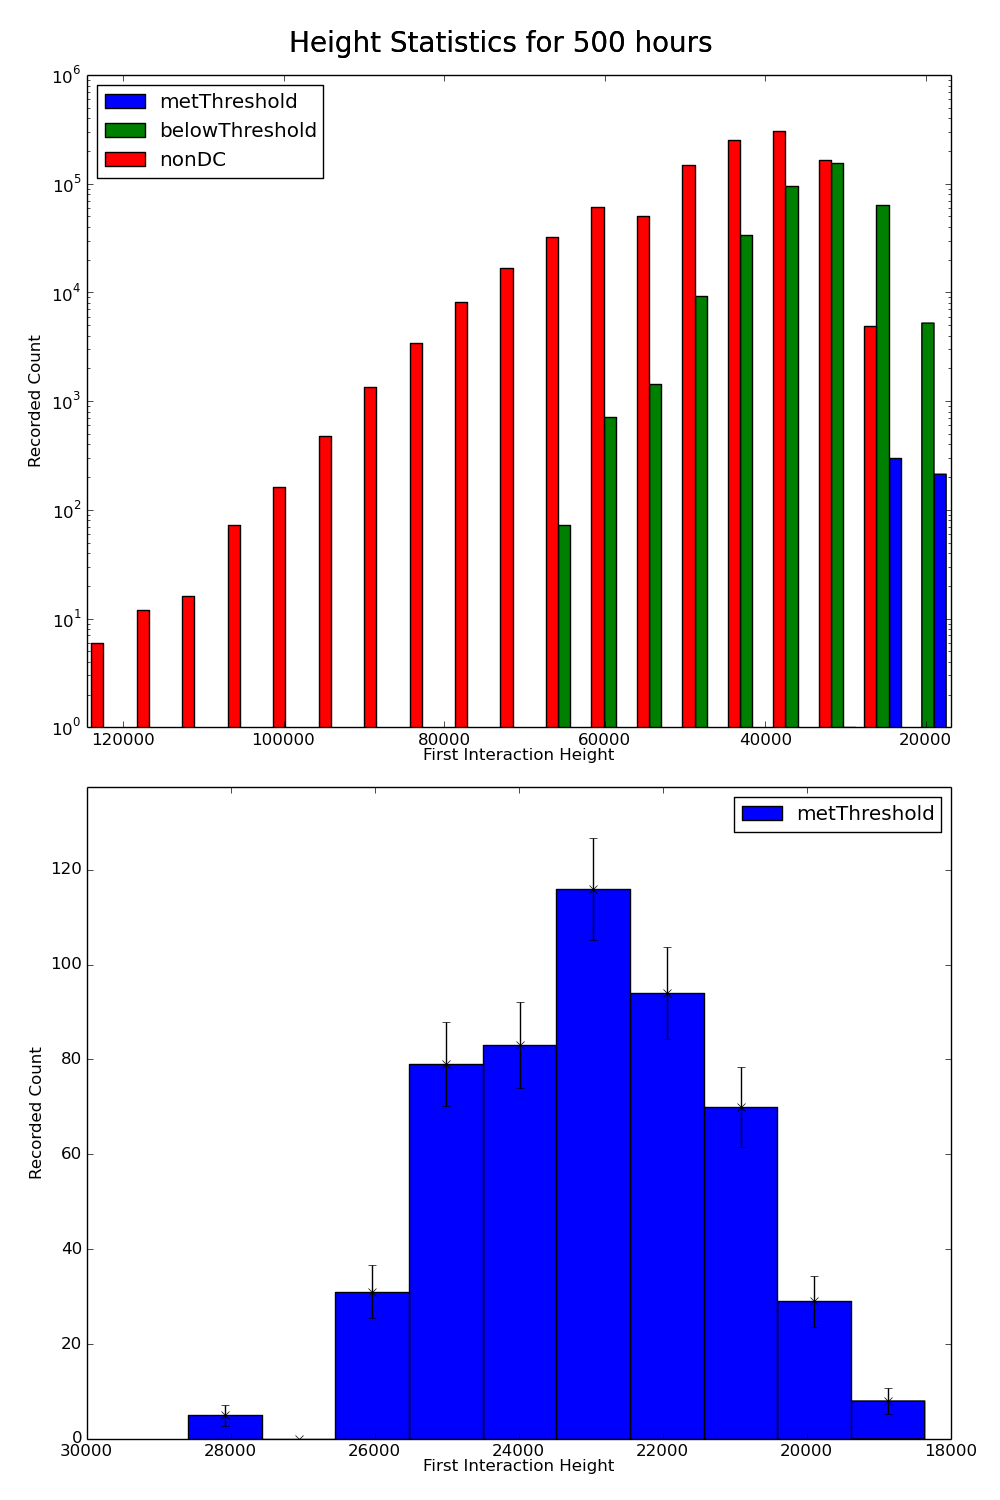
\includegraphics[height=0.9\textheight]{hessheight}
\caption{The mean first interaction height for all Cherenkov Events is 40km???. Events in blue met the multiplicity threshold, with DC light in four telescopes. The mean first interaction height for four telescope events in the HESS array is 23km}
\label{fig:Hessheight}
\end{center}
\end{figure}

\subsection{Full-Shower LPD}
Having restricted ourselves to high-multiplicity events, we reduce our data sample to mostly images in which air shower lies relatively close to the center of the telescope field of view. We can conclude that in many of our images, the air shower will lie mostly within the telescope image. In the same way as for DC light, we can look for the existence of a Characteristic LPD describing the Total Shower Intensity, where we define $I_{tot}$=Image Amplitude. The results for high-multiplicity events at various energies is shown in Figure \ref{fig:fullshowerlpd}.

\begin{figure}
\begin{center}
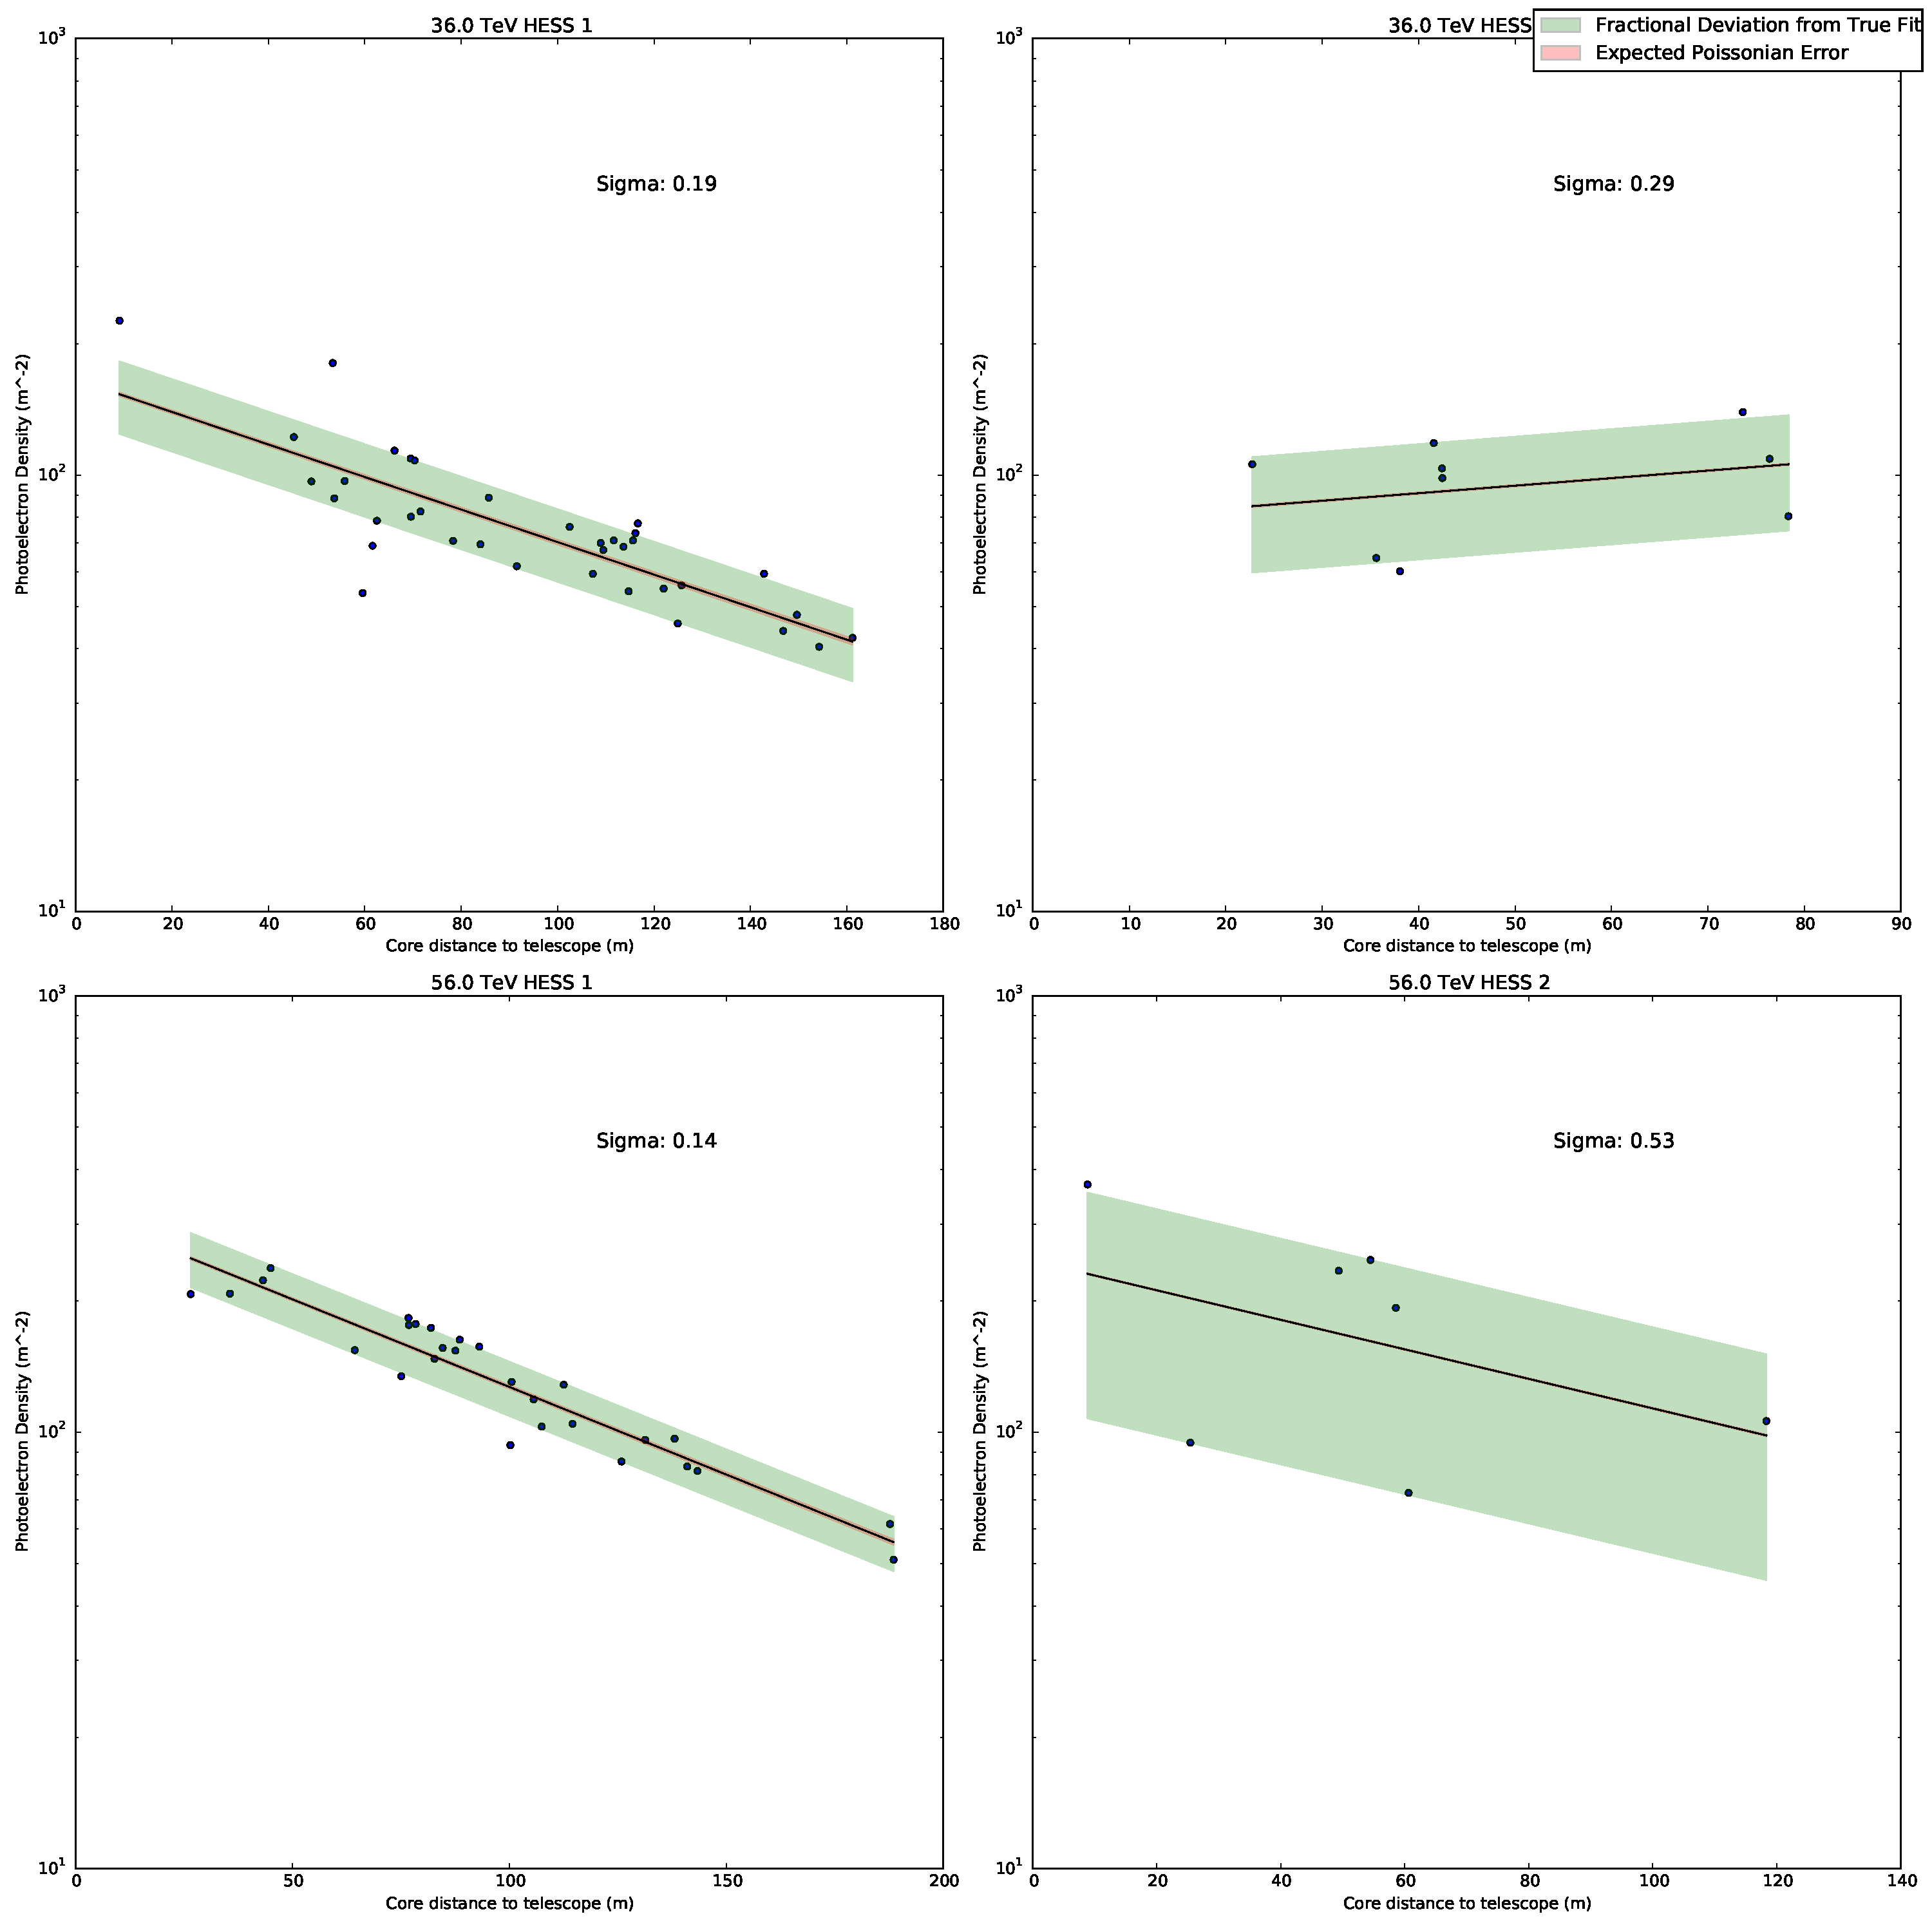
\includegraphics[width=\textwidth]{corsikafullshowerlpd}
\caption{The distribution of HESS 1 Image Amplitude is shown for various energies in the range 36-96 TeV. In each case, the exponential fit is indicated, along with the fractional deviation band in green.}
\label{fig:fullshowerlpd}
\end{center}
\end{figure}

For each energy, a clear exponential decay in Image Amplitude is observed. The data is fitted with a line of the form $y_{i} (x) =A_{i} \exp (K_{i} x)$. The fractional deviation from the fit is found in an analogous way to the DC LPD found in Figure \ref{fig:corsikalpd1}. Across all Energies, the mean fractional deviation from the fitted exponential was roughly 0.15. For the purposes of reconstruction, an exponential decay with a varying exponent and amplitude will not be particularly useful, because there are two degrees of freedom.

In order to overcome this, we can instead parameterise the exponential fits. Across all energies, a fit is made and the exponent coefficients are recorded. A plot of the $K_{i}$ exponent values is then made, as shown in Figure  \ref{fig:powerlawlpd}. The K coefficients follow a clear linear distribution, to which a line is fitted. We obtain an equation to determine the exponent of each power law. 

\[ K_{i} = K(E_{i}) = -0.00004 E_{i} + -0.00692 \]

Having retrieved a law for K, each dataset is then fitted a second time. The exponent is determined by the Energy, leaving only one degree of freedom for the fit. The fitted Amplitudes $A_{i}$ are then recorded, and are also plotted in Figure \ref{fig:powerlawlpd}. A clear exponential relationship is again observed. A straight line is fitted to the logarithm of the data values, and we retrieve a second relationship describing the amplitude as a function of the Energy.

\[ A_{i} = A(E_{i}) =y =73.9 \times \exp (0.025 E_{i}) \]

Through combined use of the two equations, we can parameterise the entire Full-Shower LPD using only the Energy. These fitted LPDs are also plotted in Figure \ref{fig:fullshowerlpd}. The fractional deviation bands are also shown in green, with a mean fractional deviation of roughly 0.15 across the energies. The Full Shower LPDs continue to be large enough to trigger telescopes for several hundred meters. It is thus likely that, for high-multiplicity events, we will obtain an additional four or five data points from the Full Shower LPD.

Although the Full Shower LPDs do not depend upon the charge of the primary particle, they will still enable the core position and energy to be effectively constrained. We can use the Full Shower LPD to obtain a rough estimate for the core position, and thus a rough estimate of the distance from each telescope to the core. similarly the core energy can be estimated. Although this reconstruction will be inferior to one accounting for both LPDs, we can make use of the preliminary core position estimate to aid our calculation of $True_{DC}$. This in turn should reduce the uncertainty when determining the charge of the primary particle.

\begin{figure}
\begin{center}
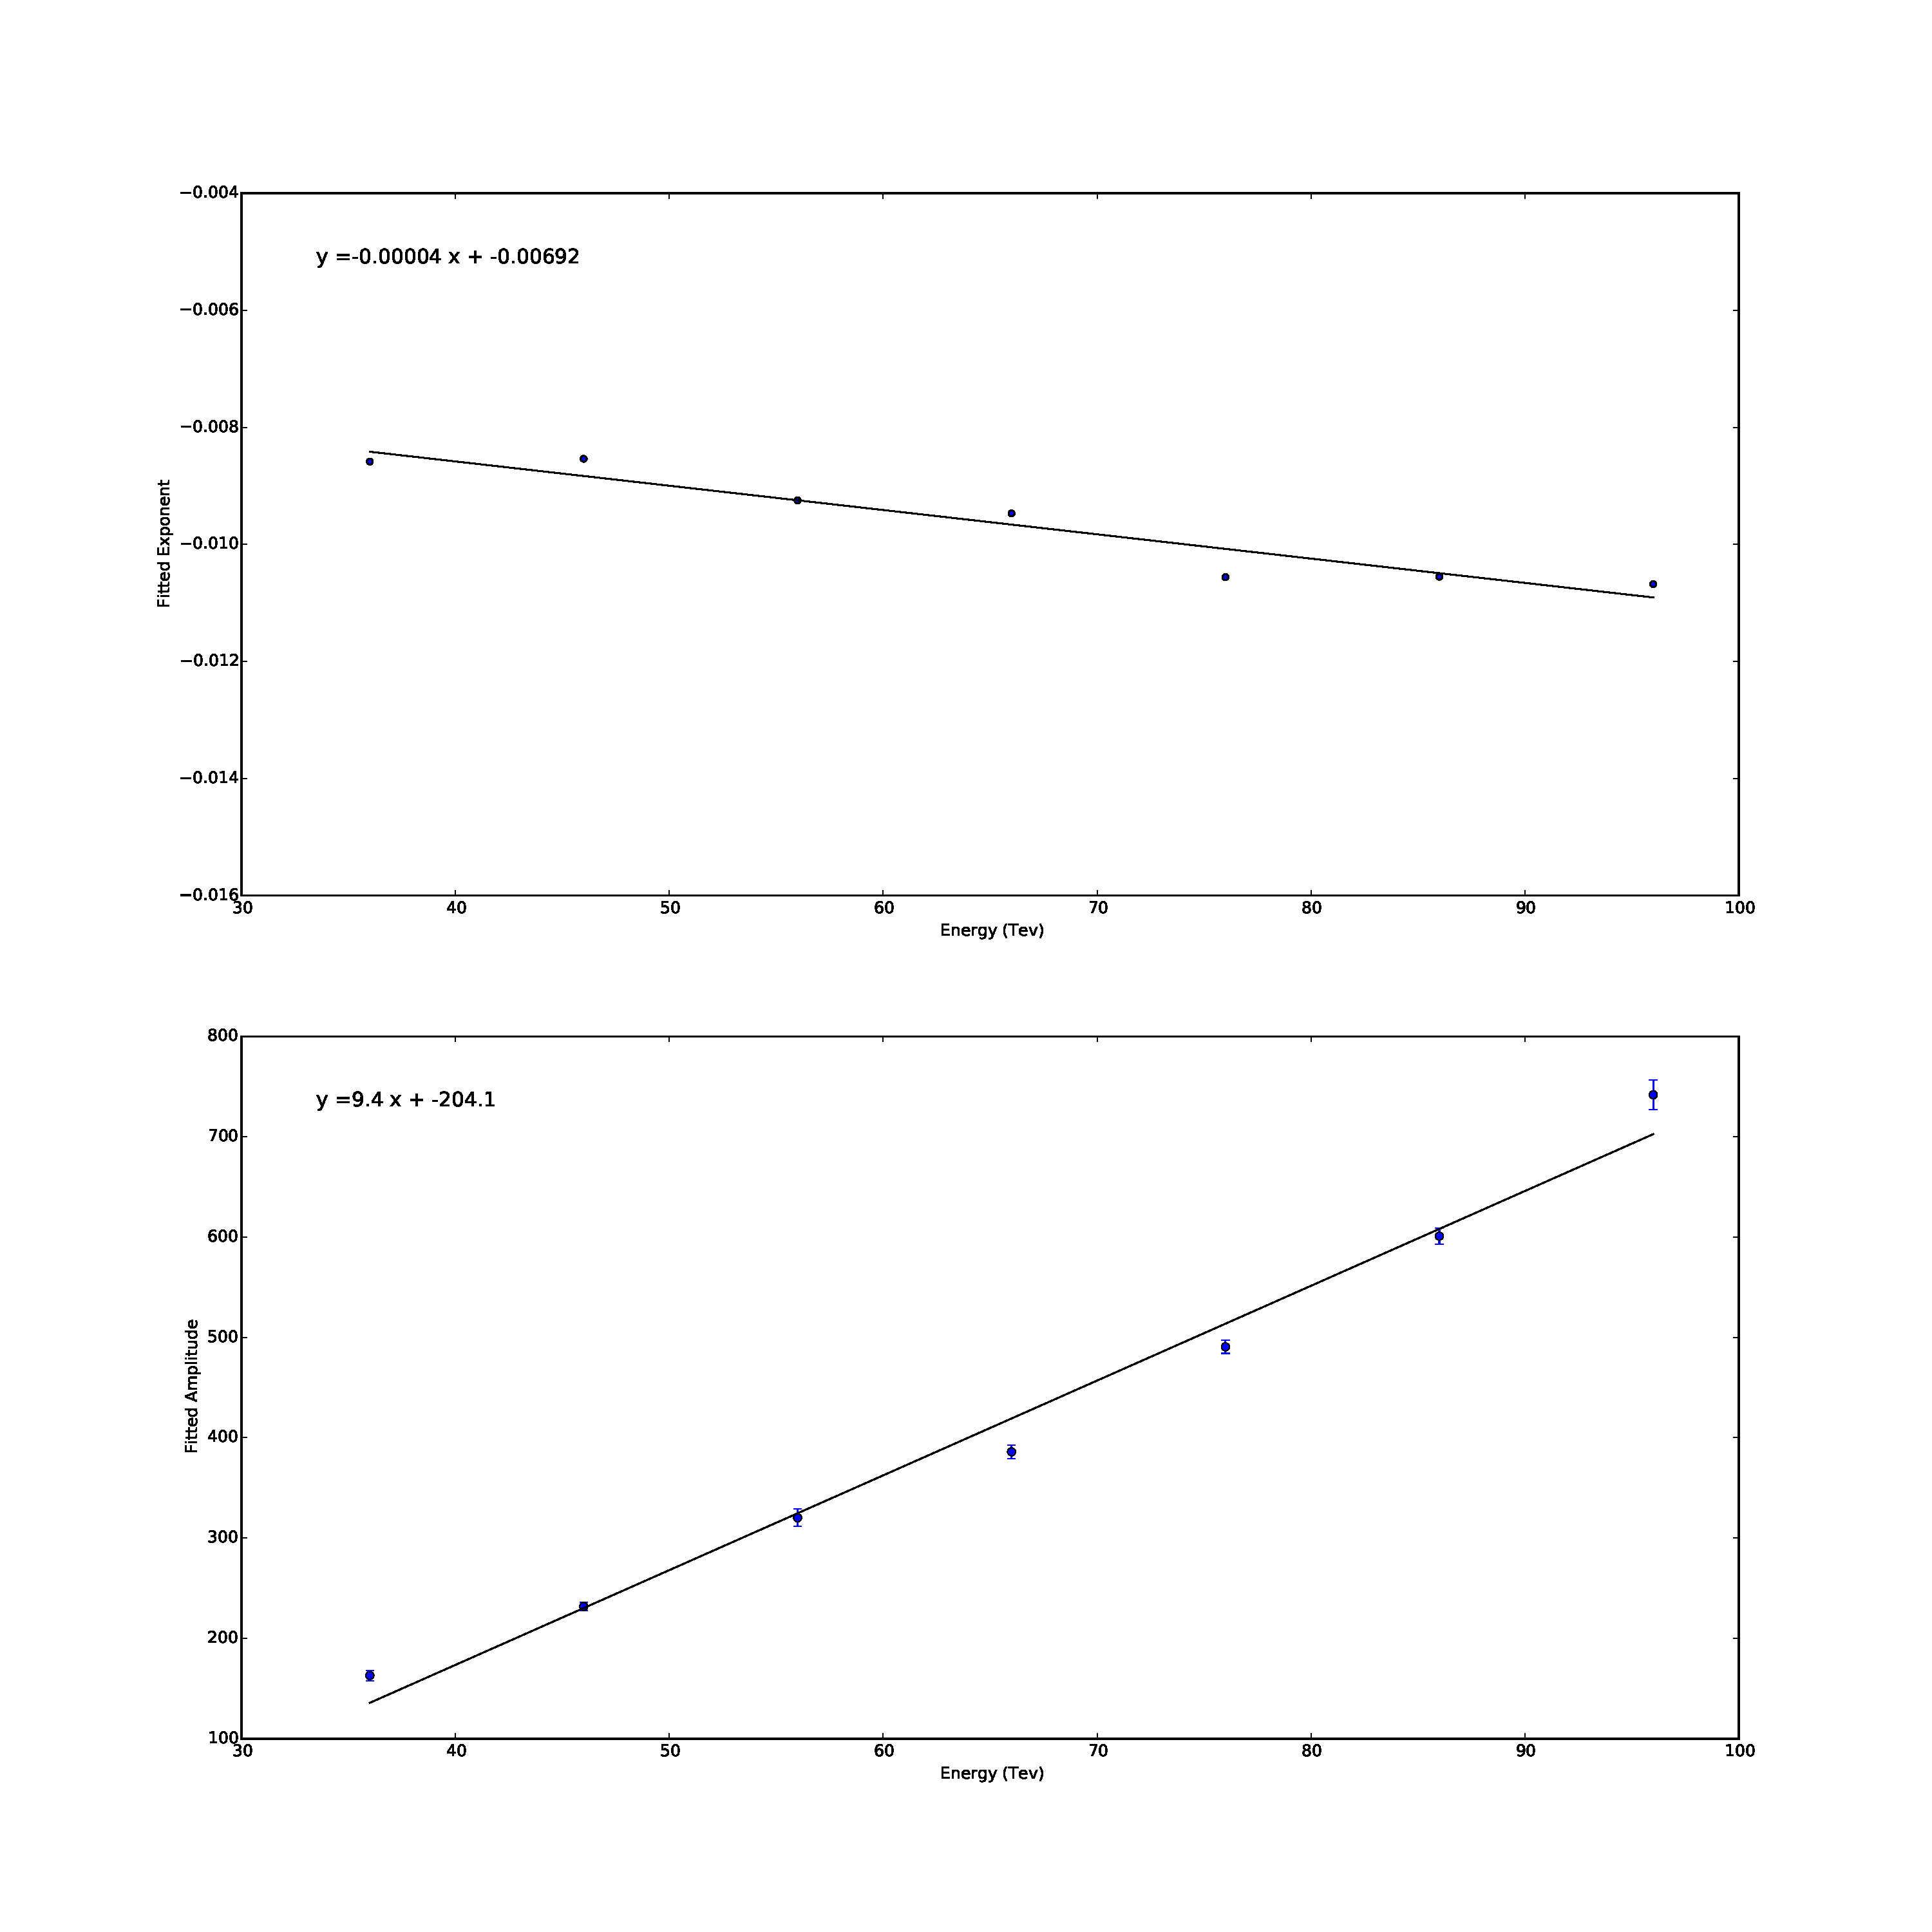
\includegraphics[width=\textwidth]{lpdpowerlaw}
\caption{The fitted exponents $K_{i}$ are shown above, along with the equation of the Fitted Exponent Line K(E). Once the fitted exponents are used, the resultant amplitudes $A_{i}$ are shown below, along with the fitted Amplitude Line A(E).}
\label{fig:powerlawlpd}
\end{center}
\end{figure}

\subsection{Determining $True_{DC}$}
Determining the value of $True_{DC}$ is essential for determining the error in our LPD measurements. However, there are two natural ways of quantifying $True_{DC}$. In the basic case, we can simply consider the EAS-free intensity $Intensity_{max}$ in the DC pixel. An alternative is to take the entire EAS-free image amplitude $I_{tot}$ as our $True_{DC}$ value. The use of Image Amplitude accounts for the fact that the DC light is almost always split between two or more pixels. Although in most cases, one pixel has the majority of the light, in extreme cases the light can be evenly split between two. As a result of the smaller angular region covered by each CT5 pixel, this happens much more frequently for HESS2 than for HESS1. A countervailing argument is the susceptibility of the Image Amplitude measurement to edge effects. A DC pixel lying near the image edge will be unaffected by this fact, but the total image amplitude may decline because dimmer pixels move over the image edge. We hope that, as with the full-shower LPD measurements, restricting ourselves to high-multiplicity events will enable us to remove most images that would otherwise suffer from edge effects.

To quantitatively compare the two methods, we can measure the error associated with both values of $True_{DC}$. A study of 2000 events was conducted, in which each cosmic ray was simulation without night sky background or EAS background. Each telescope image simulation was conducted twice, and difference between $I_{1}$ and $I_{2}$ was plotted as in \ref{fig:simtelerror}. The fractional difference from the mean Intensity of an image was defined as $\Delta = 2 \times \frac{I_{2} - I_{1}}{{I_{2} + I_{1}}}$. 

For $I_{tot}$, it was found that the standard deviation in fractional difference was $\sigma_{Itot}=0.06$, meaning that there is an inherent error of 6 \% in measurements of $True_{DC}$. In later calculations of the error in Intensity, this fractional error can be subtracted in quadrature. The distribution did not vary between HESS1 and HESS2 telescopes. For the alternative $Intensity_{max}$ measurement, the standard deviation was $\sigma_{Imax}=0.09$ for HESS1 and $\sigma_{Imax}=0.12$, a clear increase. This implies that the $I_{tot}$ measurements are more reliable.

For an alternative measurement of error in the LPD, a simulation of 2000 events was conducted with a fixed energy of 56TeV. The interaction height was allowed to vary realistically. The true distance to core was recorded from Sim\textunderscore telarray, and a graph was plotted of DC pixel intensity against core distance. As expected, a characteristic LPD is observed, as seen in Figure \ref{fig:corsikalpd1}. Due to the trigger cut on HESS cameras of 20 photoelectrons, we are only able to see the LPD from around $r_{core} \textgreater 30m$, at which point the LPD intensity crosses the threshold of 20 p.e. All telescope images lying within the maximum DC radius $r_{max}$ are marked in black, where the value of $r_{max}$ varies with energy and first interaction height. We expect these events to follow the clear theoretical LPD observed in Figure \ref{fig:lpd}. After the first interaction, further emission be determined by a highly variable fragmentation process. These events are plotted in red, and will be ignored for LPD fitting purposes. 

A parameterisation of the form $y = A \exp (b x) + C $ is fitted to the measurements of $True_{DC}$. The fractional deviation $\Delta_{TrueDC} = \frac{signal_{fit} - True_{DC count}}{signal_{fit}}$ can then be found. Using the 68th centile of all absolute fractional deviations $\Delta_{TrueDC}$, we find that the HESS LPD for $I_{tot}$ has an error of $\sigma_{Itot}=0.35$. Repeating for $Intensity_{max}$ calculated values, the resultant LPD had an error of $\sigma_{Imax} = 0.40$. Again, it is clear that the $I_{tot}$ value has a smaller associated error than $Intensity_{max}$.

It is interesting to note that the values of $I_{max}$ and $DC_{count}$ are strongly correlated with one another. The mean fractional deviation between $I_{max}$ and $DC_{count}$ is relatively small, at 0.34. It is found that the $I_{max}$ value, and by extension the $DC_{count}$ value, consistently underestimates the quantity of DC light in an image. This is not surprising, and indicates the degree to which DC light is often split between multiple pixels. As this effect is clearly not negligible, we choose to define $True_{DC}=I_{tot}$ for the rest of this analysis.

We must find the error $\sigma_{LPD}$ in our calculated values for $candidate_{DC count}$, through comparison with the correct value $True_{DC}$. However, $True_{DC}$ also has an associated error $\sigma_{STA}$, originating in the use of internal random numbers for Sim\textunderscore telarray simulations. If we neglect to account for this $\sigma_{STA}$, our final $\sigma_{calculated}$ will be an overestimate that also includes the random fluctuation of $True_{DC}$ around the actual DC intensity. As we cannot directly measure the actual DC intensity, we must instead measure $\sigma_{TrueDC}$. Having selected a method for determining $True_{DC}$, we can use the associated value of $\sigma_{STA}=0.06$. In later calculations of the error in Intensity, this fractional error can be subtracted in quadrature. 

\[ \sigma_{LPD}^{2} = \sigma_{calculated}^{2} - \sigma_{STA}^{2}  \]

\begin{figure}
\begin{center}
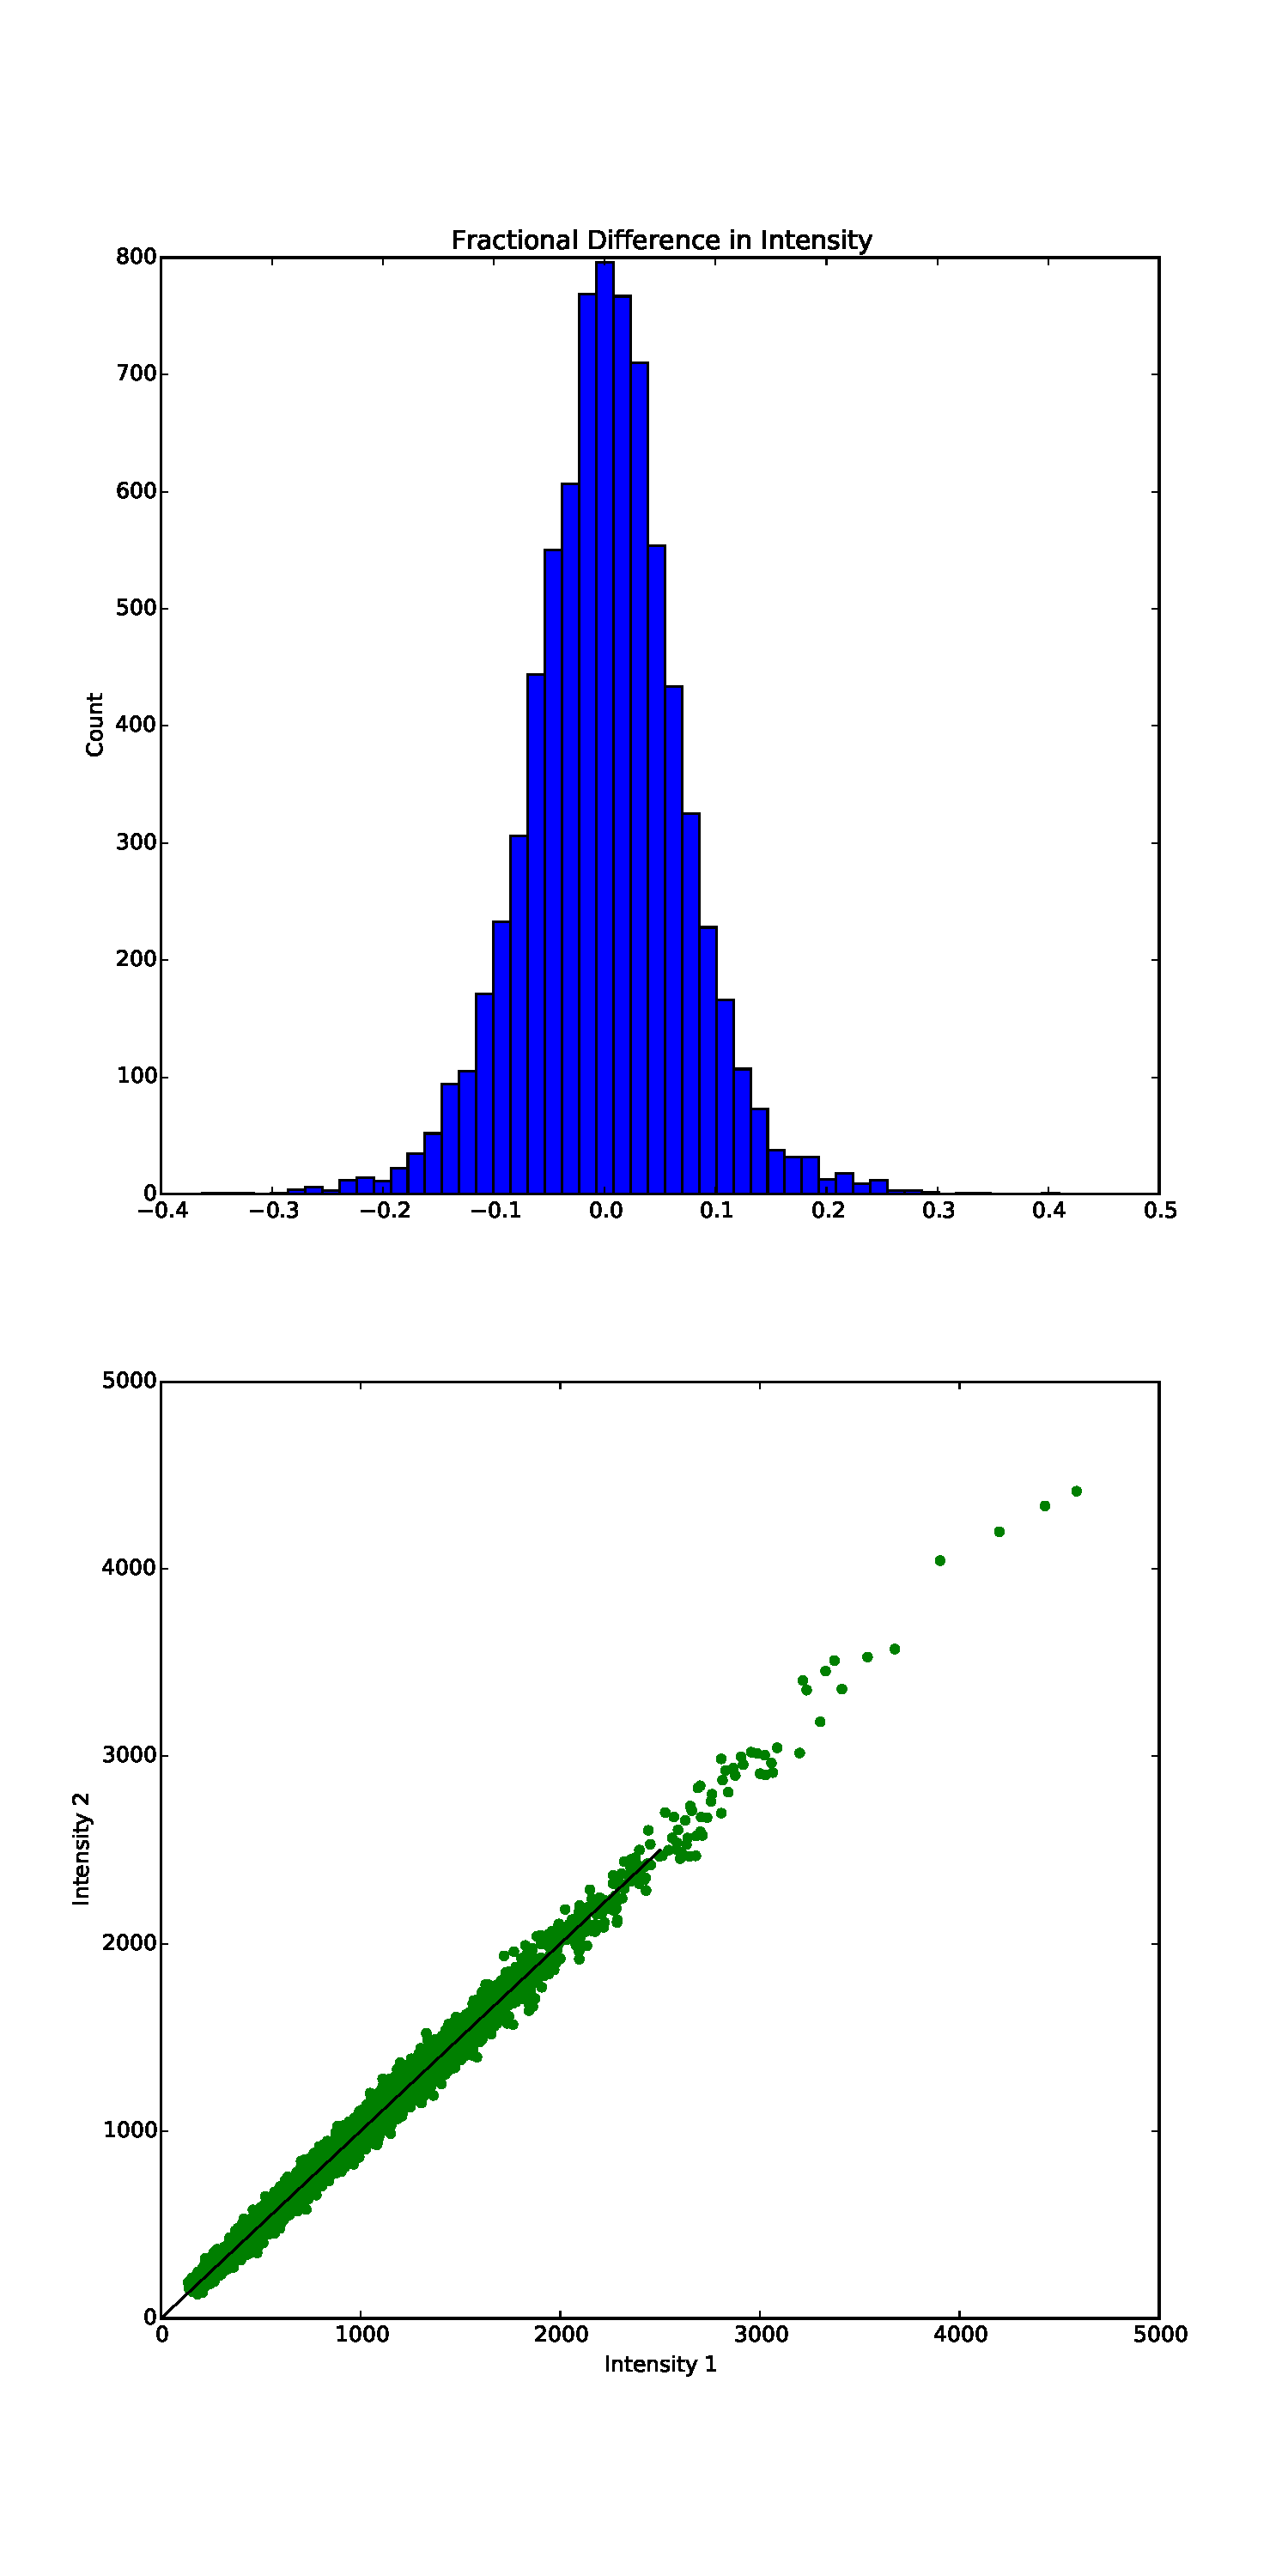
\includegraphics[height=0.9\textheight]{simtelerror1}
\caption{The fractional difference in total Image Intensity between the two simulations is shown in the graph above. A clear symmetric Gaussian is observed, with a mean of 0.00, and a standard deviation of 0.06. Below, the two intensities are plotted against one another. The distribution does not deviate significantly from the ideal 1:1 correspondence illustrated with the black line.}
\label{fig:simtelerror}
\end{center}
\end{figure} 

REDO STATS

Taking account of $\sigma_{STA}$, we deduce that the true associated error in the LPD is $\sigma_{TrueLPD} = \sqrt{(\sigma_{TrueDC}^{2} - \sigma_{STA}^{2})} = 0.11$. Thus we conclude that, in an ideal case, any LPD measuring pure DC light would always have a minimum error of 11\%. This is reasonably high, and can be partially explained by the random nature of atmospheric conditions, among other things.

The same exercise was repeated using the value of $DC_{Count}$ for the BDT candidate pixels in a full shower image, if the pixel had passed both the $DC_{Count}$ and $P_{signal}$ cuts. This provides a more reasonable estimate of the expected LPD error likely to be obtained experimentally, and includes the additional complication of having incorrectly identified pixels in the dataset. As before, the absolute fractional deviation of each pixel from the fit of the $True_{DC}$ LPD was found. Due to consistent underestimate of the $True_{DC}$ value using the simple $DC_{Count}$ method, the error was much larger, with $\sigma_{DCcount}=0.57$ and the $\sigma_{STA}$ being negligible in comparison. This representative error is extremely large, and will pose significant problems for event reconstruction.

\begin{figure}
\begin{center}
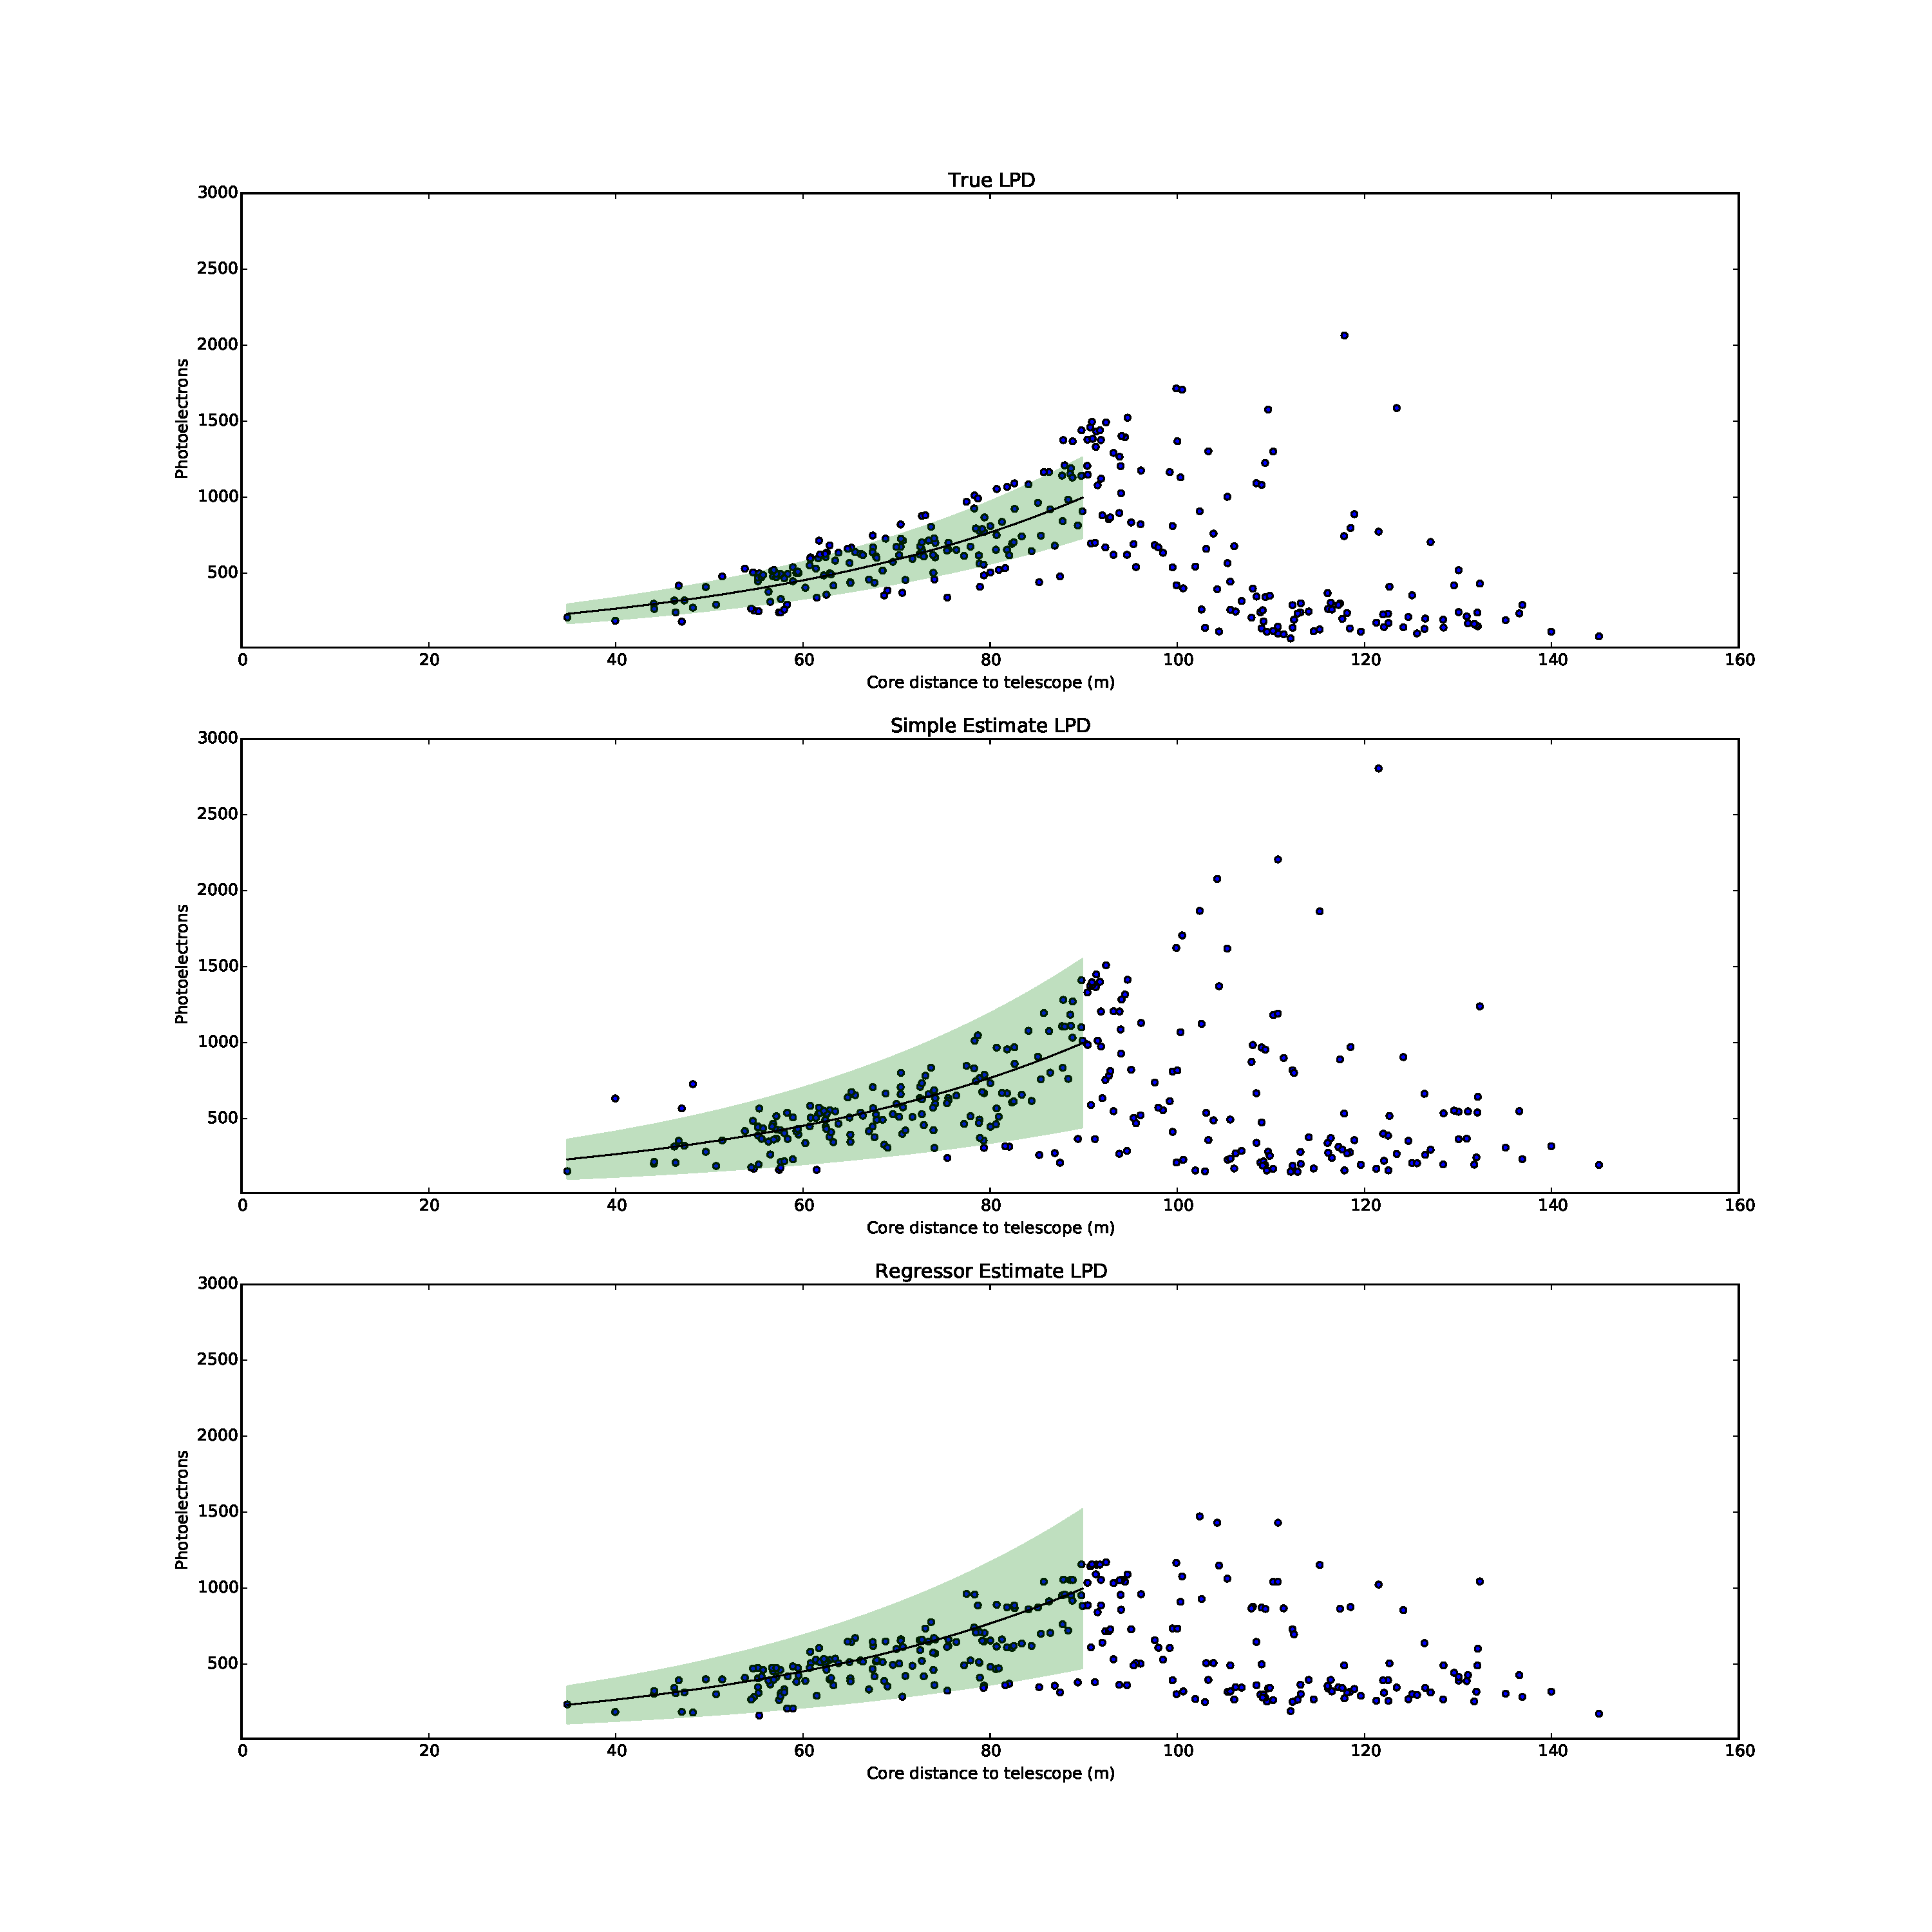
\includegraphics[width=\textwidth]{corsikalpd1}
\caption{The two LPDs shown above are estimates of HESS1 $True_{DC}$ calculated via $I_{tot}$, as well as for the maximum pixel $Intensity$. The two full-shower calculated LPDSs are shown underneath, with the simple guess $DC_{Count}$, and the regressor calculated $DC_{rgr}$. An exponential is fit to the $True_{DC}$ distribution, and the 68\% fractional deviation is shown in green. The same curve is shown on the two derived DC values, with the new fractional deviation being much greater.}
\label{fig:corsikalpd1}
\end{center}
\end{figure}

\subsection{Regression BDT for $DC_{Count}$}
In order to reduce the LPD error, an alternative method of calculating the DC signal was developed. Supervised machine learning was again used to solve the problem, through training of a BDT Regressor. As with Classifiers, Regressors are initially trained using individual data entries. Instead of the true classes for the entries, regressors require the true value of a continuous variable. Once trained, the Regressor can be used to predict a value of the variable for a given data entry. In this case, the Regressor is trained to estimate the quantity of DC light $True_{DC}$ for a given pixel. Once a DC pixel has been identified, the Regressor is applied to it. The Regressor returns the calculated value of $DC_{rgr}$, an alternative estimate of the DC signal. 

Accurate measurement of the value of $True_{DC}$ is hindered because the DC light can be split into multiple pixels. Instead of the brightest pixel intensity the total Image Amplitude in the EAS free image was used. However, for high altitude/zenith angles, the DC light may lie partially outside the telescope image. To remove all associated uncertainty, a fitted parameterisation was used based on the LPD for $True_{DC}$.

\[ y_{1}(r<r_{max}) = \frac{Z}{26}^{2} \times 5.3 \times \exp(0.013 r)\]
\[ y_{2}(r > r_{max}) = y_{1}(r_{max}) \times \exp (-0.06( r-r_{max})) \]

For convenience, an offset $C=-6.5$ was omitted, yielding a simple exponential law. Counter-intuitively, it does in fact not matter whether the training values bear any close relation to the $True_DC$ values. The only values that we can use for reconstruction are our $candidate_{DC count}$, based on the DC candidate pixel and full-shower image. As long as these $candidate_{DC count}$ values are proportional to $Z^{2}$, the reconstruction method will remain valid. We train the regressor to interpolate the value of $True_{DC}$ using a number of variables, and most importantly, we include the True distance to the Core and the true energy among the regressor variables listed in Table \ref{tab:regressor}. 

In theory, any parameterisation would be valid for the regressor to train with. It is obvious that, if given accurate core distance values, the regressor will always be able to perfectly replicate the exponential distribution. However, we cannot give a trained regressor true values of energy or distance to the core, when the regressor is applied to experimental images. Instead, we must give an approximation of these values, estimated through analysis of the full shower. Thus, if we were to choose a completely outlandish parameterisation that did not correlate to the images at all, the only useful variable would be the true core distance. As we do not exactly know the core distance, we would also have a large uncertainty in $candidate_{DC count}$. Because no additional information would be present in the resultant LPD, any reconstruction would not provide reduction in core position or charge resolution measurement. 

If suitably trained, the regressor would consider the core position as a factor, but also correlate it with other variable related to the image. Then, given an estimate of the core distance, the regressor is able to produce a value of $candidate_{DC count}$ with some small error, that is still proportional to $Z^{2}$. The training set of data consisted of one true DC pixel entry in each full shower image. 

The training sample contains, in equal proportion, elements Manganese (Z=25), Iron (Z=26) and Cobalt (Z=27). This to ensure that the regressor is well trained to distinguish between different cosmic ray charges, by providing variation of $Z^{2}$ for training. If the regressor is capable of distinguishing between these three elements, then this will serve as a sufficient proof of concept. We expect that, were an entire spectrum of cosmic ray elements simulated, a regressor could be trained with similar performance for a large charge range. The training of such a BDT was not done as part of this analysis, due to computing time restraints. However, in Monte Carlo simulations, the existence of a regressor will be assumed.

To account for the differing hardware, a separate regressor was trained, as before, for the CT5 camera. The Feature Importances for the HESS1 and HESS2 regressor are listed in Table \ref{tab:regressor}.. There is little discrepancy in variable importance between the two BDTs.

\begin{table}[h!]
  \centering
  \caption{Relative Feature Importance in  Regressor BDT training}
  \label{tab:regressor}
  \begin{tabular}{ccc}
    \toprule
    Variable & HESS-1 & HESS-2 \\
    \midrule
    Aspect Ratio & 0.12 & 0.12\\
    $Intensity_{N.N.min}$ & 0.11 & 0.12\\
    Image Amplitude & 0.11 & 0.11\\
    $Q_{DC}$ & 0.10 & 0.11\\
    $r_{core}$ & 0.10 & 0.10\\
    $Intensity_{N.N.max}$ & 0.10 & 0.10\\
    $Mean_{N.N}$ & 0.10 & 0.09\\
    Energy & 0.09 & 0.09\\
    $DC_{Count}$ & 0.09 & 0.09\\
    $Intensity$ & 0.08 & 0.08\\
    \bottomrule
  \end{tabular}
\end{table}

The features importances are, on the face of it, rather surprising. Ultimately, the true values for energy and $r_{core}$ are not the most important variables. We can conclude that the regressor has been well taught to indirectly infer the cosmic ray charge, and account for this by correlating values to the true core distance/energy. The Aspect Ratio is heavily dependent on distance to core, but also on the charge. Thus, in combination with $r_{core}$, the charge can be reasonably inferred. Similarly the Image Amplitude is relied upon to infer energy, and in conjunction with the estimated energy, can indicate charge. It is encouraging to see that the regressor relies more heavily on Image Amplitude and Aspect Ratio, because these two values are known with a much smaller uncertainty than the core position/energy.

Repeating the comparison for the HESS1 regressor, we find for $\sigma_{rgr} = 0.14$, a significant improvement over $\sigma_{DCcount}$. The plotted LPD is seen in Figure \ref{fig:corsikalpd1}. Through use of a well-defined law for the training values, we have eliminated the influence of $\sigma_{STA}$ on the training process. The comparative performance is recorded in Table \ref{tab:lpderror}.

Instead of rejecting DC pixels which do not meet out $DC_{count}$ and $P_{signal}$ cuts, we can separately measure their deviation from the LPD. In this way, we can include the information from these DC pixels in later analysis, while accounting for the larger uncertainty in their LPD measurements. For images which do pass only the multiplicity cuts, but not the $P_{signal}$ or $DC_{count}$ cuts, we find that the regressor error is $\sigma_{rejected1}=0.15$. We can thus make use of these points, because they follow an almost identical distribution. 

STUFF

\begin{table}[h!]
  \centering
  \caption{Fractional error from fitted 56-TeV LPD distribution up to $r_{core}=90$, accounting for $\sigma_{STA}$}
  \label{tab:lpderror}
  \begin{tabular}{ccc}
    \toprule
    & HESS1 & HESS2\\
    \midrule
    $\sigma_{TrueDC}$ & 0.13 & 0.29\\
    $\sigma_{DCcount}$ & 0.69 & 0.91\\
    $\sigma_{rgr}$ & 0.27 & 0.53\\ 
    $\sigma_{rejected}$ & 0.32 & 0.43\\ 
    \bottomrule
  \end{tabular}
\end{table}

\section{Monte Carlo Simulation}
Having obtained a parameterisation for both the full and DC LPD, as well as the associated error in the case of a HESS-type array, the Charge reconstruction Technique can be applied to a simpified Monte Carlo simulation of the HESS array, developed as part of this analysis. Conducting a Monte Carlo simulation using the Gaussian-smeared LPD, we can measure the effectiveness of the LPD-reconstruction technique. The simulated Cosmic Rays must be high-multiplicity, and have a realistic distribution of energy and interaction height values.

\subsection{Iron Flux and Energy}
Iron nucleii, like all Cosmic Rays, follow a well-defined power law where $\phi(E) = \frac{dN(E)}{dt} = \phi_{0} E^{-\gamma} $ for some constant k. Using the SIBYLL model for Cosmic Ray Simulation, we assume that $ \gamma = 2.76 \pm 0.11 $ and $\phi_{0}=0.029 \pm 0.01 m^{-2} s^{-1} sr^{-1} TeV ^{-1}$ \cite{hess07}. Considering the same Energy Range of 35-135 TeV, we can calculate the integrated Iron Flux. 

\[ F(35-135TeV) = \int_{35}^{135} \phi_{0} E^{-2.76} dE = \frac{\phi_{0}}{1.76}[35^{-1.76} - 135^{-1.76}] = 2.86 \times 10^{-5} m^{-2} s^{-1} sr^{-1}\]

Within CORSIKA, a square simulation of 300 x 300m was simulated. We can consider an identical $90000 m^{2}$ target region for core position simulation. The HESS telescope additionally has a solid and field of view of 5 degrees (0.09 rad),meaning an expected telescope array Iron Flux of $F(35-135TeV) = 0.22 s^{-1}$. On the basis of efficiency calculations in DC pixel identification, it is clear that 2.2\% of Iron Ray events will produce high-multiplicity DC pixels accepted by the BDT. Thus, we will ultimately obtain an hourly flux of $F(35-135TeV) = 4.84 \times 10^{-3} s^{-1} = 17.4 h^{-1}$ high-multiplicity Iron events. 

The full 5-telescope HESS array has been in operation since 2012 \cite{hessCT5}, and has thus had time to collect several years of data. Due to the requirement of night operation under favourable weather conditions, the HESS phase 2 experiment has collected approximately 5000 hours of data. On the basis of our high-multiplicity flux rate, we can assume that a rough expected event count would be roughly 7900 high-multiplicity iron events. The Monte Carlo simulations will be run with approximately this number of events.

To accurately model the Cosmic Rays, the Energy Power Law must be simulated. To generate the random Energy value En(R) following the power law, a uniformly distributed random number R is generated. The value of R represents a random fraction of the total simulated flux $ F(R) = R \times F(35-135TeV) $, and can thus range from 0-1. Having determined the Integrated Flux corresponding to the random number, the Energy corresponding to this flux can be calculated. The energy E is defined as the lower bound of the integral which would produce the chosen integrated flux F. Thus R=0 corresponds to an Energy of 135TeV yielding no Integrated Flux, while R=1 would correspond to an Energy of 35TeV and the full Integrated Flux. THus the simulated Cosmic Rays will obey the power law, with high-energy events being realistically suppressed.

\[ F(R) = F(En(R)-135TeV) = \int_{En(R)}^{135} \phi_{0} E^{-2.76} dE =\frac{\phi_{0}}{1.76}[En(R)^{-1.76} - 135^{-1.76}]= R \times F(35-135TeV)\] \[\Longrightarrow  En(R) = (\frac{1.76\times R \times F(35-135TeV)}{\phi_{0}} +135^{-1.76})^{\frac{-1}{1.76}} \]

RATES!!!

\subsection{First Interaction Height}
Cosmic Rays survival in from the top of the atmosphere follows an exponential decay with the number of 'interaction lengths' passed. 

The mean free path $\ell$ of a Cosmic Ray is a function of atmospheric cross section and number density, which are themselves functions of  height, so that $\ell(h) = \frac{1}{\sigma(h) n(h)}$. It is instead easier to consider a new variable x, which we name the \textquoteleft Interaction Distance', so that the survival probability of a cosmic ray follows a simple exponential decay with the interaction distance passed. We thus define one Interaction Length, $x_{0}$ such that a cosmic ray traveling through one interaction length will have a non-interaction probability of $\frac{1}{e}$, and in general $P_{survival} \propto e^{\frac{-x}{x_{0}}}$ The geometric distance corresponding to one interaction length will vary as a function of height.

The Interaction Length is inversely proportional to the interaction cross section, which is itself proportional to local atmospheric number density, so that $x_{0} \propto \frac{1}{n(h)}$. Thus, because the number density of the atmosphere increases with decreasing height, the local interaction length will be geometrically shortened as the height of the cosmic ray decreases. If we consider the Integrated Interaction Distance as the total number of interaction lengths passed by a Cosmic Ray from the top of the atmosphere to a given height h, we see in Figure \ref{fig:generalheight} that the total integrated interaction distance increases exponentially with increasing height. We use the standard HESS-based data tables also found in the CORSIKA software, containing information regarding the integrated interaction distance and refractive index over a range of heights. As a function of x, the corresponding local interaction rate $\Gamma_{interact}(x)$ will be a product of the survival probability and the probability of interacting $P_{interact}(x)= -\frac{dP_{survival}(x)}{dx}$. 

\[ \Gamma_{interact}(x) = P_{interact} \times N_{survived} =  - \frac{dP_{survival}(x)}{dx} \times (N \times  P_{survival}) \]

The fraction of surviving and interacting cosmic rays are shown in Figure \ref{fig:generalheight}, alongside the resultant distribution of interactions binned by height h rather than interaction length x. The height of each bin can be considered an average local value for $\Gamma_{interact}(h)$, and it is clear that the function $\Gamma_{interact}(h)$ peaks at a height of around 40km. This is thus the height region where most of our cosmic rays will interact with the atmosphere.

\begin{figure}
\begin{center}
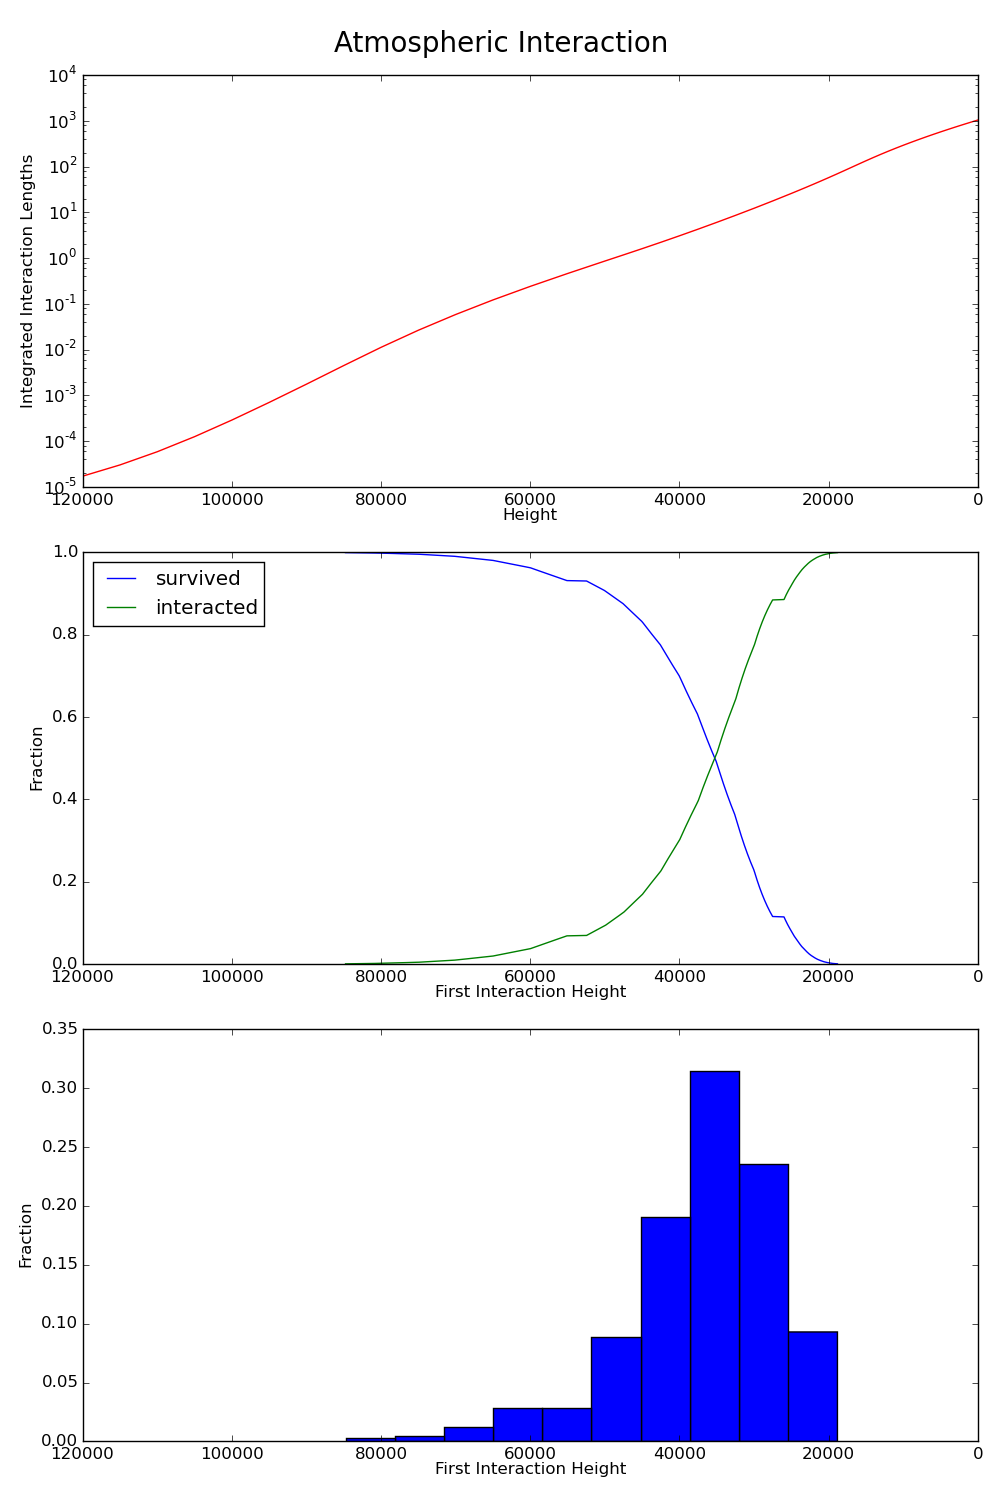
\includegraphics[height=0.9\textheight]{generalheight}
\caption{The integrated interaction lengths increases as height decreases. Thus the decay probability follows a exponentially increasing distribution. The mean first interaction height for all events is roughly 40km above sea level.}
\label{fig:generalheight}
\end{center}
\end{figure}

To simulate the First Interaction Height, we assign a uniform random number R to each event, corresponding to the $P_{survival}$ at which the cosmic ray will interact. R can be interpreted fraction of events that will have interacted before the simulated cosmic ray does. It ranges from R=0 for interaction at the top of the Atmosphere to R=1 for an event reaching the ground. Having determined the fraction of events, we assume the survival probability is normalised. As with all exponential distributions, we see that the expectation value is equal to one Interaction Length.

\[ P_{survival}(x) = k e^{\frac{-x}{x_{0}}} \Longrightarrow \int_{0}^{\infty} P_{survival}(x) dx = k x_{0} [ e^{0} - e ^ {- \infty}] = 1 \Longrightarrow k = \frac{1}{x_{0}}\]
\[P_{half}(x) =\int_{0}^{x_{median}} k e^{\frac{-x}{x_{0}}} dx =[1 -e^{\frac{-x_{median}}{x_{0}}} ]= \frac{1}{2} \Longrightarrow {x_{median}} = x_{0} \ln (2)\]

\[ <x> =  \int_{0}^{\infty} P_{survival}(x) dx = x_{0} = \frac{x_{median}}{\ln (2)} \]

Thus, we can simply calculate $x_{0}$ as the expectation value of interaction length. This parameter is free-floating, and can only be determined through experimental study of Cosmic Rays. Experimental results indicate an approximate cross section of $\sigma_{Fe-air} = 2000mb$ and a corresponding thus $x_{0} \approx 12 g cm^{-2}$ \cite{Montanus2013}. 

As with energy, we wish to simulate a realistic spectrum for the first interaction heights. We must thus convert the uniform random number R to an interaction distance X. Using the standard atmospheric tables, the corresponding height value can be found using exponential interpolation. The standard atmospheric data is included in the appendix.

\[ R = \int_{0}^{X} k e^{\frac{-x}{x_{0}}} dx = [1 -e^{\frac{-X}{x_{0}}}] \Longrightarrow X = -x_{0} \ln (1 - R) \] 

Interpolating the value of the height neglects the fact that some cosmic rays which would not interact with the atmosphere before reaching the ground. The integrated interaction lengths are equal to about 850 at an altitude comparable to the HESS site. There is thus a probability of reaching the ground equal to $P = exp(\frac{-850}{12}) \approx 1.73 \times 10 ^{-31}$. It is thus reasonable to ignore this tiny fraction of events, and instead assume that every cosmic ray will interact at some point in the atmosphere.

As cited by the HESS study, a typical first interaction height is roughly 30km for a Cherenkov-Emitting event \cite{hess07}. With the assumed value of $x_{0}$, a simulation was conducted to determine the expected interaction heights for Cosmic Rays. It is found that the mean first interaction height of 36.9km and a median first interaction height of 35.2km for all cosmic rays. However, when Cherenkov-Emitting events are considered, we have both a median and mean first interaction height of 30.3km, which clearly agrees with our expectations. Considering solely high-multiplicity events, we find that these have a mean height of $h \approx 23 \pm 5$ km, as shown in Figure \ref{fig:Hessheight}.

Another parameter exponentially interpolated using the data tables is the optical depth to the surface, $\tau$. The Cherenkov Light, mostly emitted in the visible blue part of the EM spectrum, experiences relatively little atmospheric absorption. The major of Rayleigh scattering-based atmospheric absorption occurs in the lower part of the troposphere, and thus the atmospheric absorption is almost independent of emission up to first interaction height. For a given emitted intensity $I_{0}$ we find that the corresponding I received on the ground decays exponentially with optical depth, so that $\frac{I}{I_{0}}=e^{-\tau}$ with $\tau=\int_{0}^{l}ds$. 

MOAR!!!

\subsection{Full-Shower event reconstruction}
The full shower image amplitude seen in a telescope depends on the core position and the core energy. We have determined a very clear parameterisation of this LPD, along with the expected LPD fractional deviation of $\frac{\sigma_{I}}{I}= 0.15$. The received full shower amplitude is simulated under the assumption of a Gaussian distribution around the expected value. We can thus reconstruct the core position and energy using a Log Likelihood minimisation. Once a Cosmic Ray has reached saturation, the Cherenkov Emission is effectively independent of its energy, barring determination of the first interaction height. Consequently, the energy value is solely determined by the full-shower amplitudes. 

Having observed the full shower in n telescopes out of five, we consider each of the total photoelectron counts $N_{i, received}$. We aim to determine the expectation value of the LPD, $\mu(x, y, Energy$) , which led to the measurement $N_{i, received}$. For a given expectation value, we know the corresponding probability of observing $N_{i, received}$ will be the standard Gaussian probability, with a sigma of $\sigma = 0.15 \times \mu$.

\[  P_{i} ( N_{i, Received} \mid X, Y, Energy )  =  \frac{1}{\sqrt{2 \sigma^{2} \pi}} \exp(-\frac{(N_{i, Received} - \mu)^{2}}{2 \sigma^{2}}) \]

To reconstruct the event parameters, we must minimise the probability of a given set of observations. We know that the probability of obtaining a set $N_{i,received}$ will simply be the product of the probability of each individual measurement, $\mathbb{P}(x, y, Energy) = \prod_{i=1}^{n} P_{i}(x, y, Energy)$. For convenience we minimise the negative log likelihood instead, in which case we find that we can sum over the contribution of each telescope. We then minimise the function by varying the core position and energy, to find the most likely values for those parameters.

\[ - \ln(L) = - \sum_{i=1}^{n} \ln(P_{i}) =  \sum_{i=1}^{n} [ \frac{1}{2}\ln(2 \pi) + \ln(\sigma) + \frac{(N_{i, Received} - \mu)^{2}}{2 \sigma^{2}}]\]

The minimsation is done with the iMinuit python package, which calls the MINUIT algorithm to seek a minima in a multi-dimensional parameter space \cite{James75}. Due to the discontinuous nature of the likelihood function in the case of non-observation of an air shower, it is sometimes the case that the MINUIT algorithm will find a local rather than global minima. To mitigate this problem, we can start the minimisation on points in a lattice of starting values within the parameter space. In each case, we would find a local minimum and an assosiated likelihood. We can then select the local minimum with the smallest associated likelihood as the global minimum for the entire parameter space. 

Using basic Hillas reconstruction techniques we can find a rough estimate of the core position. For each telescope, we will obtain an expected direction to shower core, although it will be heavily Gaussian-smeared from the true direction. However, combining these values can restrict us to an expected target region. We consider a grid of spacing 5m in the xy plane, and with each telescope, consider the reconstructed direction to shower core. Allowing a certain angular deviation will give us a target region containing certain likely grid points. We progressively increase the angular deviation until we have found the twenty most likely core position points. It is important to note that these core positions are simply starting points for a minimisation. The minimisation itself is allowed to float freely anywhere in the simulated target grid of $300 \times 300 = 90000 m^{2}$.

In addition, with reference to the energy power law, we consider 50 starting energy values. We again use the energy range 35-135 TeV, and as with the initial simulation of the core energy, we convert probabilities to energys. In this case, the probability range 0-1 is split into 50 evenly-spaced values, and each of these is converted into a corresponding energy coordinate. Thus most of the energy values are found at the lower end of the spectrum, because this is also where the true values for most events will be found.

In combination, we consequently have a total of 1000 minimisations. Having run the minimisation algorithm, we thus acheive a full-shower LPD reconstruction, and obtain a measurement of the core energy and starting position. The resulting fraction error in energy distribution is shown below in Figure \ref{fig:rawepn}. Under the assumption of a gaussian distribution, we can calculate the mean fractional deviation as half of the distance between the 16th and 84th centiles of data. We sort each fractional deviation, and expect that 68\% of events will lie between these values. Using this method, it is clear that the energy reconstruction is fairly good, with a fractional standard deviation of roughly 0.10 when both four and five telescope events are considered. We find that the position is also reconstructed, with an accuracy of . Having now reconstructed the value of the energy with reasonable accuracy, we can make use of this value when attempting to reconstruct the DC LPD. 

\begin{figure}
\begin{center}
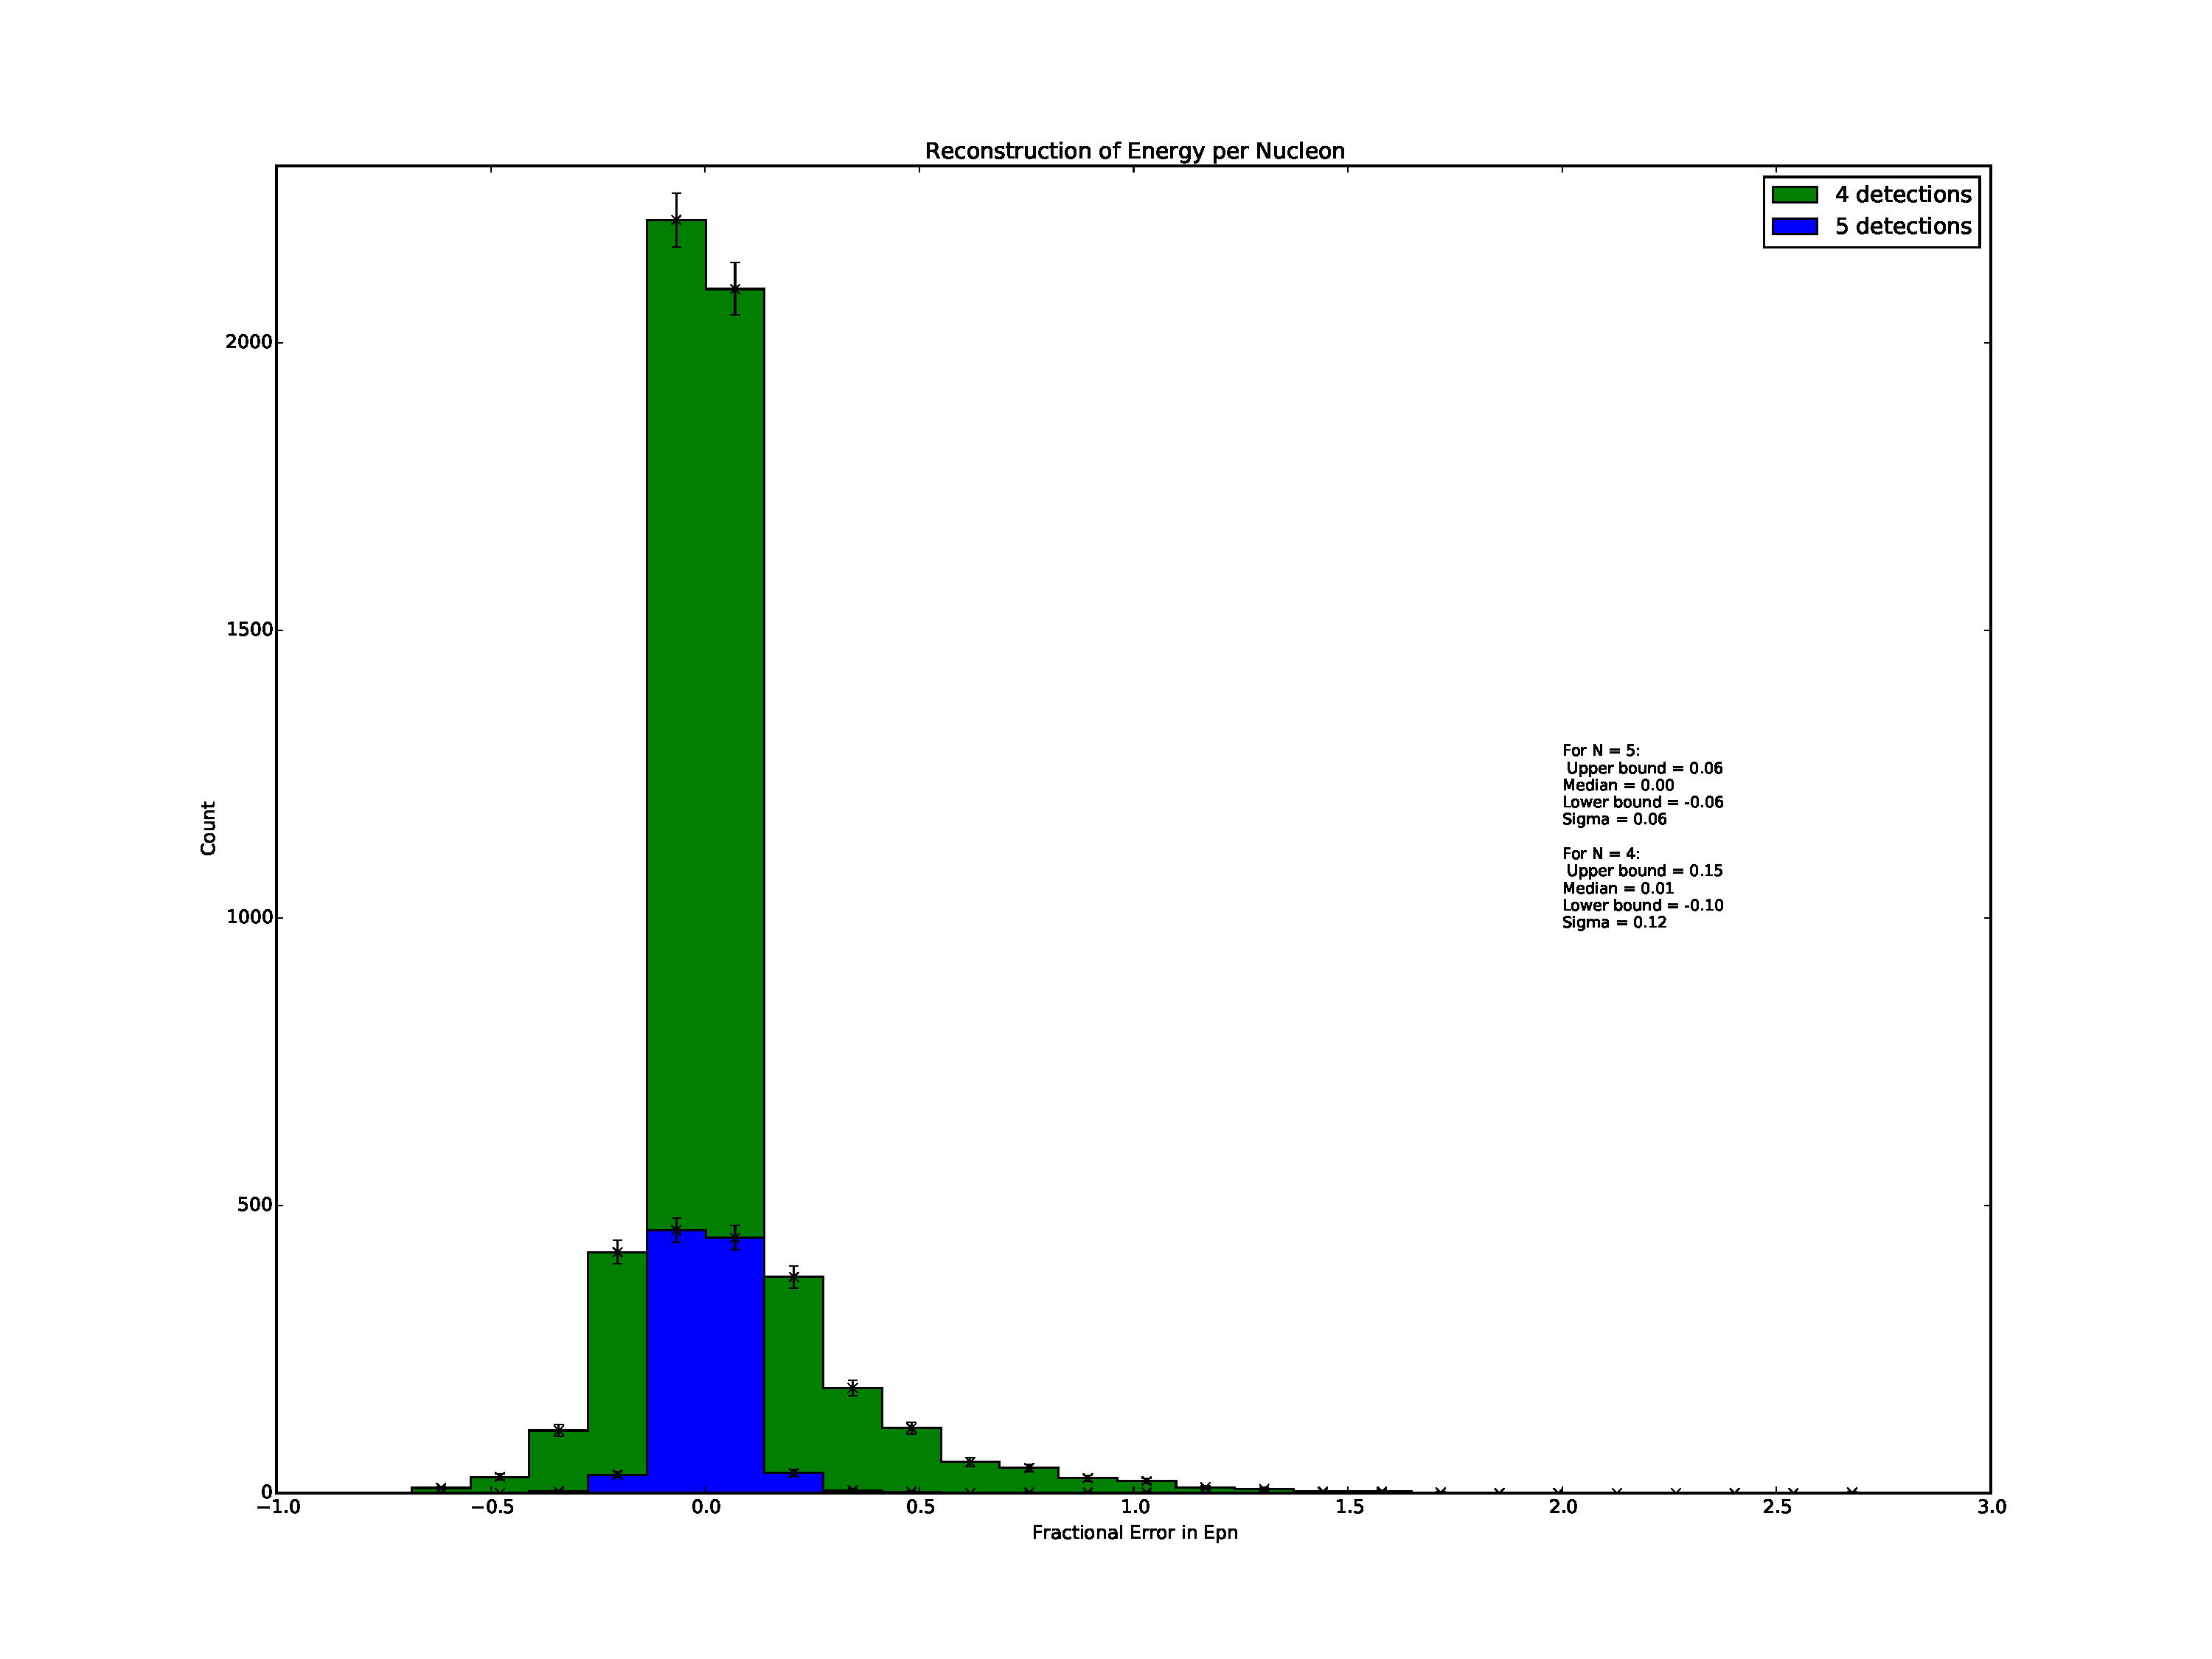
\includegraphics[width=\textwidth]{rawepn}
\caption{The fraction deviation from true energy is shown above. For events with five-telescope multiplicity, the fractional error is X but for four-telescope multiplicity, it is Y. The expected poissonian error bars are also shown.}
\label{fig:rawepn}
\end{center}
\end{figure}  
A graph showing the difference between the distance from telescope to true core position, and the distance from telescope to this reconstructed core position. Using the same 68\% method, the standard deviation from the true core distance  is 10m for 5 telescope events, and 16m for four telescope events. A better estimate for the core position will take into account the DC LPD as well as the full LPD.

\begin{figure}
\begin{center}
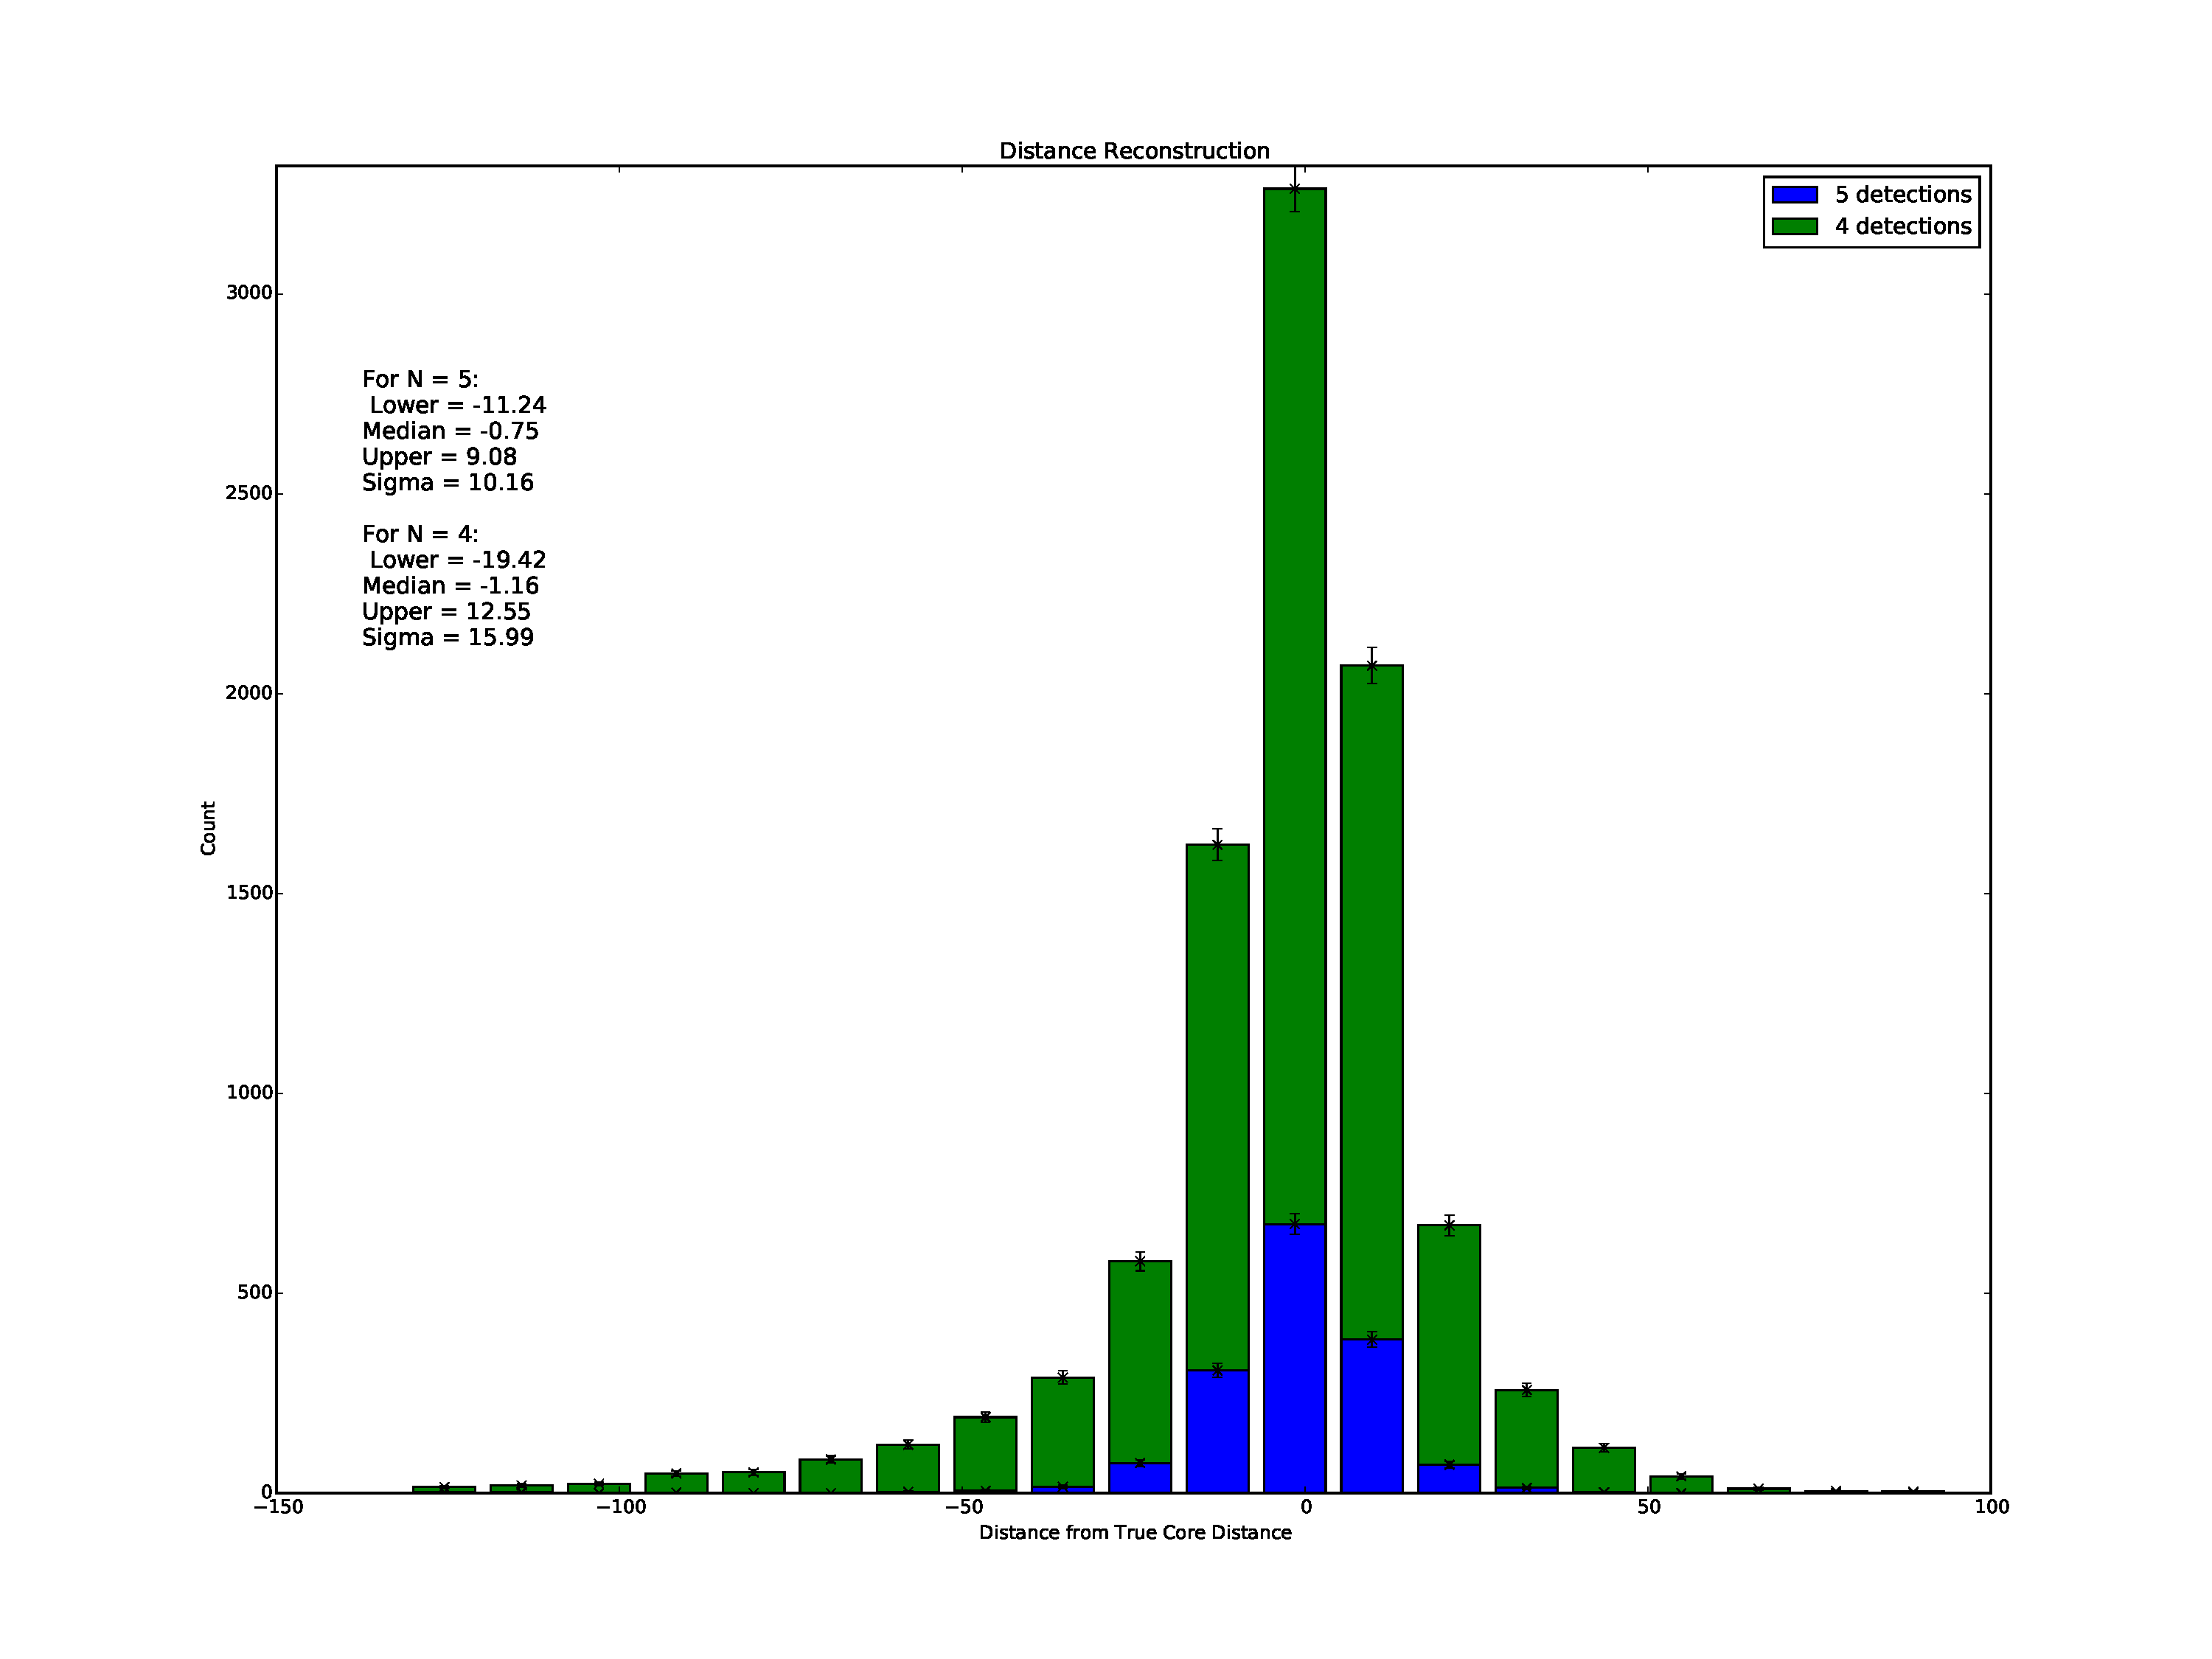
\includegraphics[width=\textwidth]{rawcoredistance}
\caption{The distance from true core to the core reconstructed with the full-LPD is shown above. For four-telescope events, the standard deviation from true position is Xm. }
\label{fig:rawcoredistance}
\end{center}
\end{figure} 

It is interesting to note that, for both variables, 5-telescope events have a lower deviation that 4-telescope events. This is despite the fact that the multiplicity refers solely to the number of identified DC pixels. The number of triggered telescopes containing an air shower is almost always five for these events, regardless of whether a DC pixel exists and can be identified. We can partially explain this by considering events which are likely to have 5 DC pixels. In such a case, the SOMETHING...

\subsection{Log Likelihood Minimisation}
Having estimated the rough core position and energy, we would at this point use our regressor to determine the values of $candidate_{DCcount}$, based on the BDT-identified DC pixel and image parameters. Having done so, we know that these values would follow the regressor LPD. For the Monte-Carlo simulation, this step is bypassed, and the regressor LPD is instead directly simulated with a standard Gaussian smearing. Having quantified the expected deviation from the LPD under these conditions, this is a reasonable simplification that massively reduces the computing requirements for event simulation. This in turn enables us to consider a greatly expanded dataset for reconstruction attempts.
 
In order to fully reconstruct the events, we need to find the x/y core position, the Energy per Nucleon, the first interaction height and the charge. We again consider the amount of DC light that each telescope receives to be Gaussian, with an expectation of $\mu(X, Y, Z, height, Epn)$ and a standard deviation of $\sigma(\mu)$. Ultimately the energy dependence of the LPD is almost negligible over the energy range, because variable $r_{max}$ is only weakly dependent on the energy. It thus makes little sense to attempt to reconstruct the energy a second time, when we would expect no discernible improvement over the reconstruction solely based on the Full Shower LPD that was performed before. We thus fix the cosmic ray energy as that found before, and instead consider a four-dimensional minimisation in Charge, x and y core position, and first interaction height.

We then minimise the Log Likelihood function, where the total log likelihood for each telescope is equal to a sum of the full-shower LPD log likelihood and the DC LPD log likelihood. We are thus minimising a Likelihood function with nine or ten measurements from two broadly independent distributions. We consequently expect an improvement in the position reconstruction, as well as a measurement of the charge and the first interaction height.

As before, we find that the discontinuous LPD leads to a frequent identification of local rather than global minima. To overcome this problem, we can iterate over a series of starting values for the parameters, with the aim of scanning the true minimum among the many minima found. In addition to the grid of likely positions identified for the Full-Shower LPD minimisation, we can can scan the integer Z values over the range $ 20 \leq Z \leq 32 $. It should be emphasised that the charge Z is treated as a free-floating parameter during the minimisation, and is able to vary freely within the range 16-36. Similarly, three first interaction heights in the range 20-30 km are scanned, but the value is able to vary freely in the range 15-65 km. It is purely due to computer resource restraints that \textquoteleft likely coordinates' in the parameter space are scanned as a starting point for a minimisation, rather than a uniformly distributed scan. Despite the simplifications, each minimisation process will still undergo $12 \times 20 \times 3 = 720$ iterations before a final reconstruction is complete. 

\subsection{Variable Resolution}
If we compare the deviation from true core distance to each telescope, we can quantify the improvcement in core position reconstruction from minimisation based solely on the full-shower LPD. This is shown in Figure \ref{fig:coredistance}, and is directly comparable with the preliminary results in Figure \ref{fig:rawcoredistance}. As expected, the core distance resolution is reduced to X and Ym, and clear improvement over the previous measurements of core position. 

\begin{figure}
\begin{center}
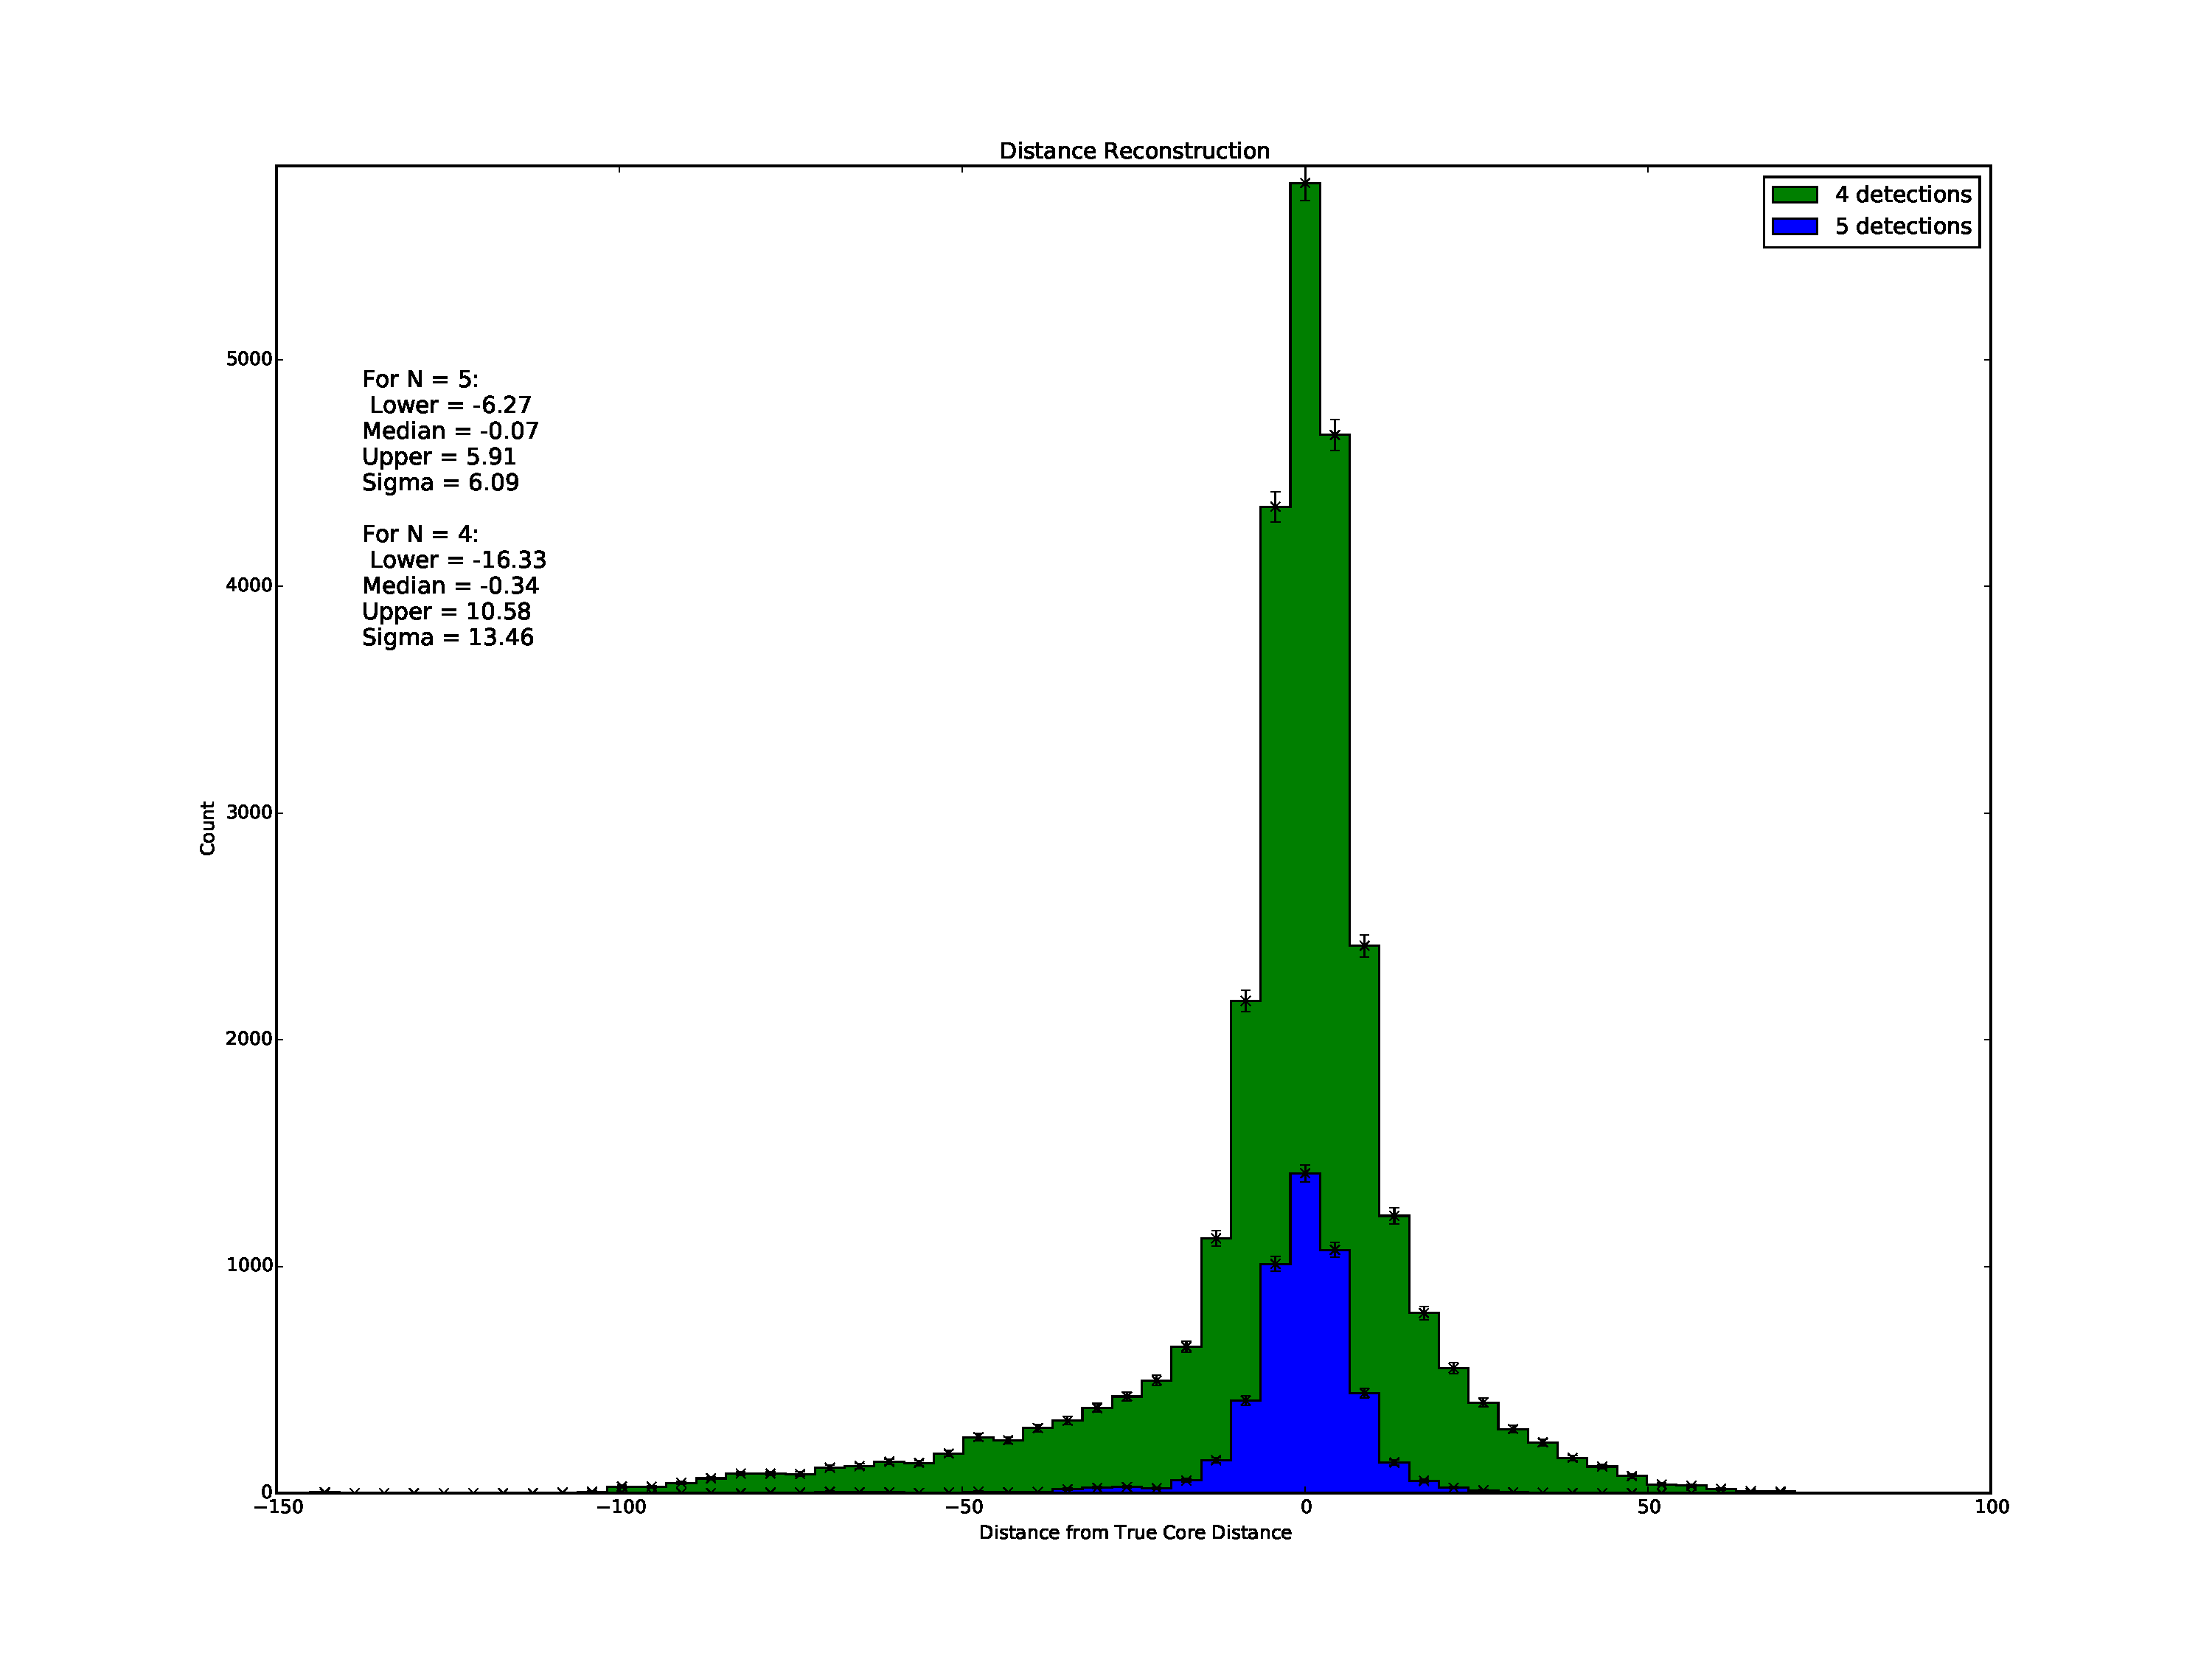
\includegraphics[width=\textwidth]{coredistance}
\caption{The distance from true core to the core reconstructed with the full-LPD is shown above. For four-telescope events, the standard deviation from true position is Xm. }
\label{fig:coredistance}
\end{center}
\end{figure}

As an alternative metric for assessing reconstruction accuracy, we can calculate the absolute distance from the reconstructed core to the true core. The results of a binning of this distribution are shown in Figure \ref{fig:position}. Because we consider absolute distance, this value can never be negative. Thus, we calculate a one-sided distribution standard deviation, and consider the value of an event in the 68th centile to be equal to the standard deviation. It is found that, for both four and five telescope events, the core reconstruction is approximately $\sigma_{core} \approx 10m$. Most reconstructed core positions thus lie less than 10m from the true position. This is extremely good, especially in comparison to the Hillas Reconstruction, where a core resolution of Y is more typical AND CITE!

\begin{figure}
\begin{center}
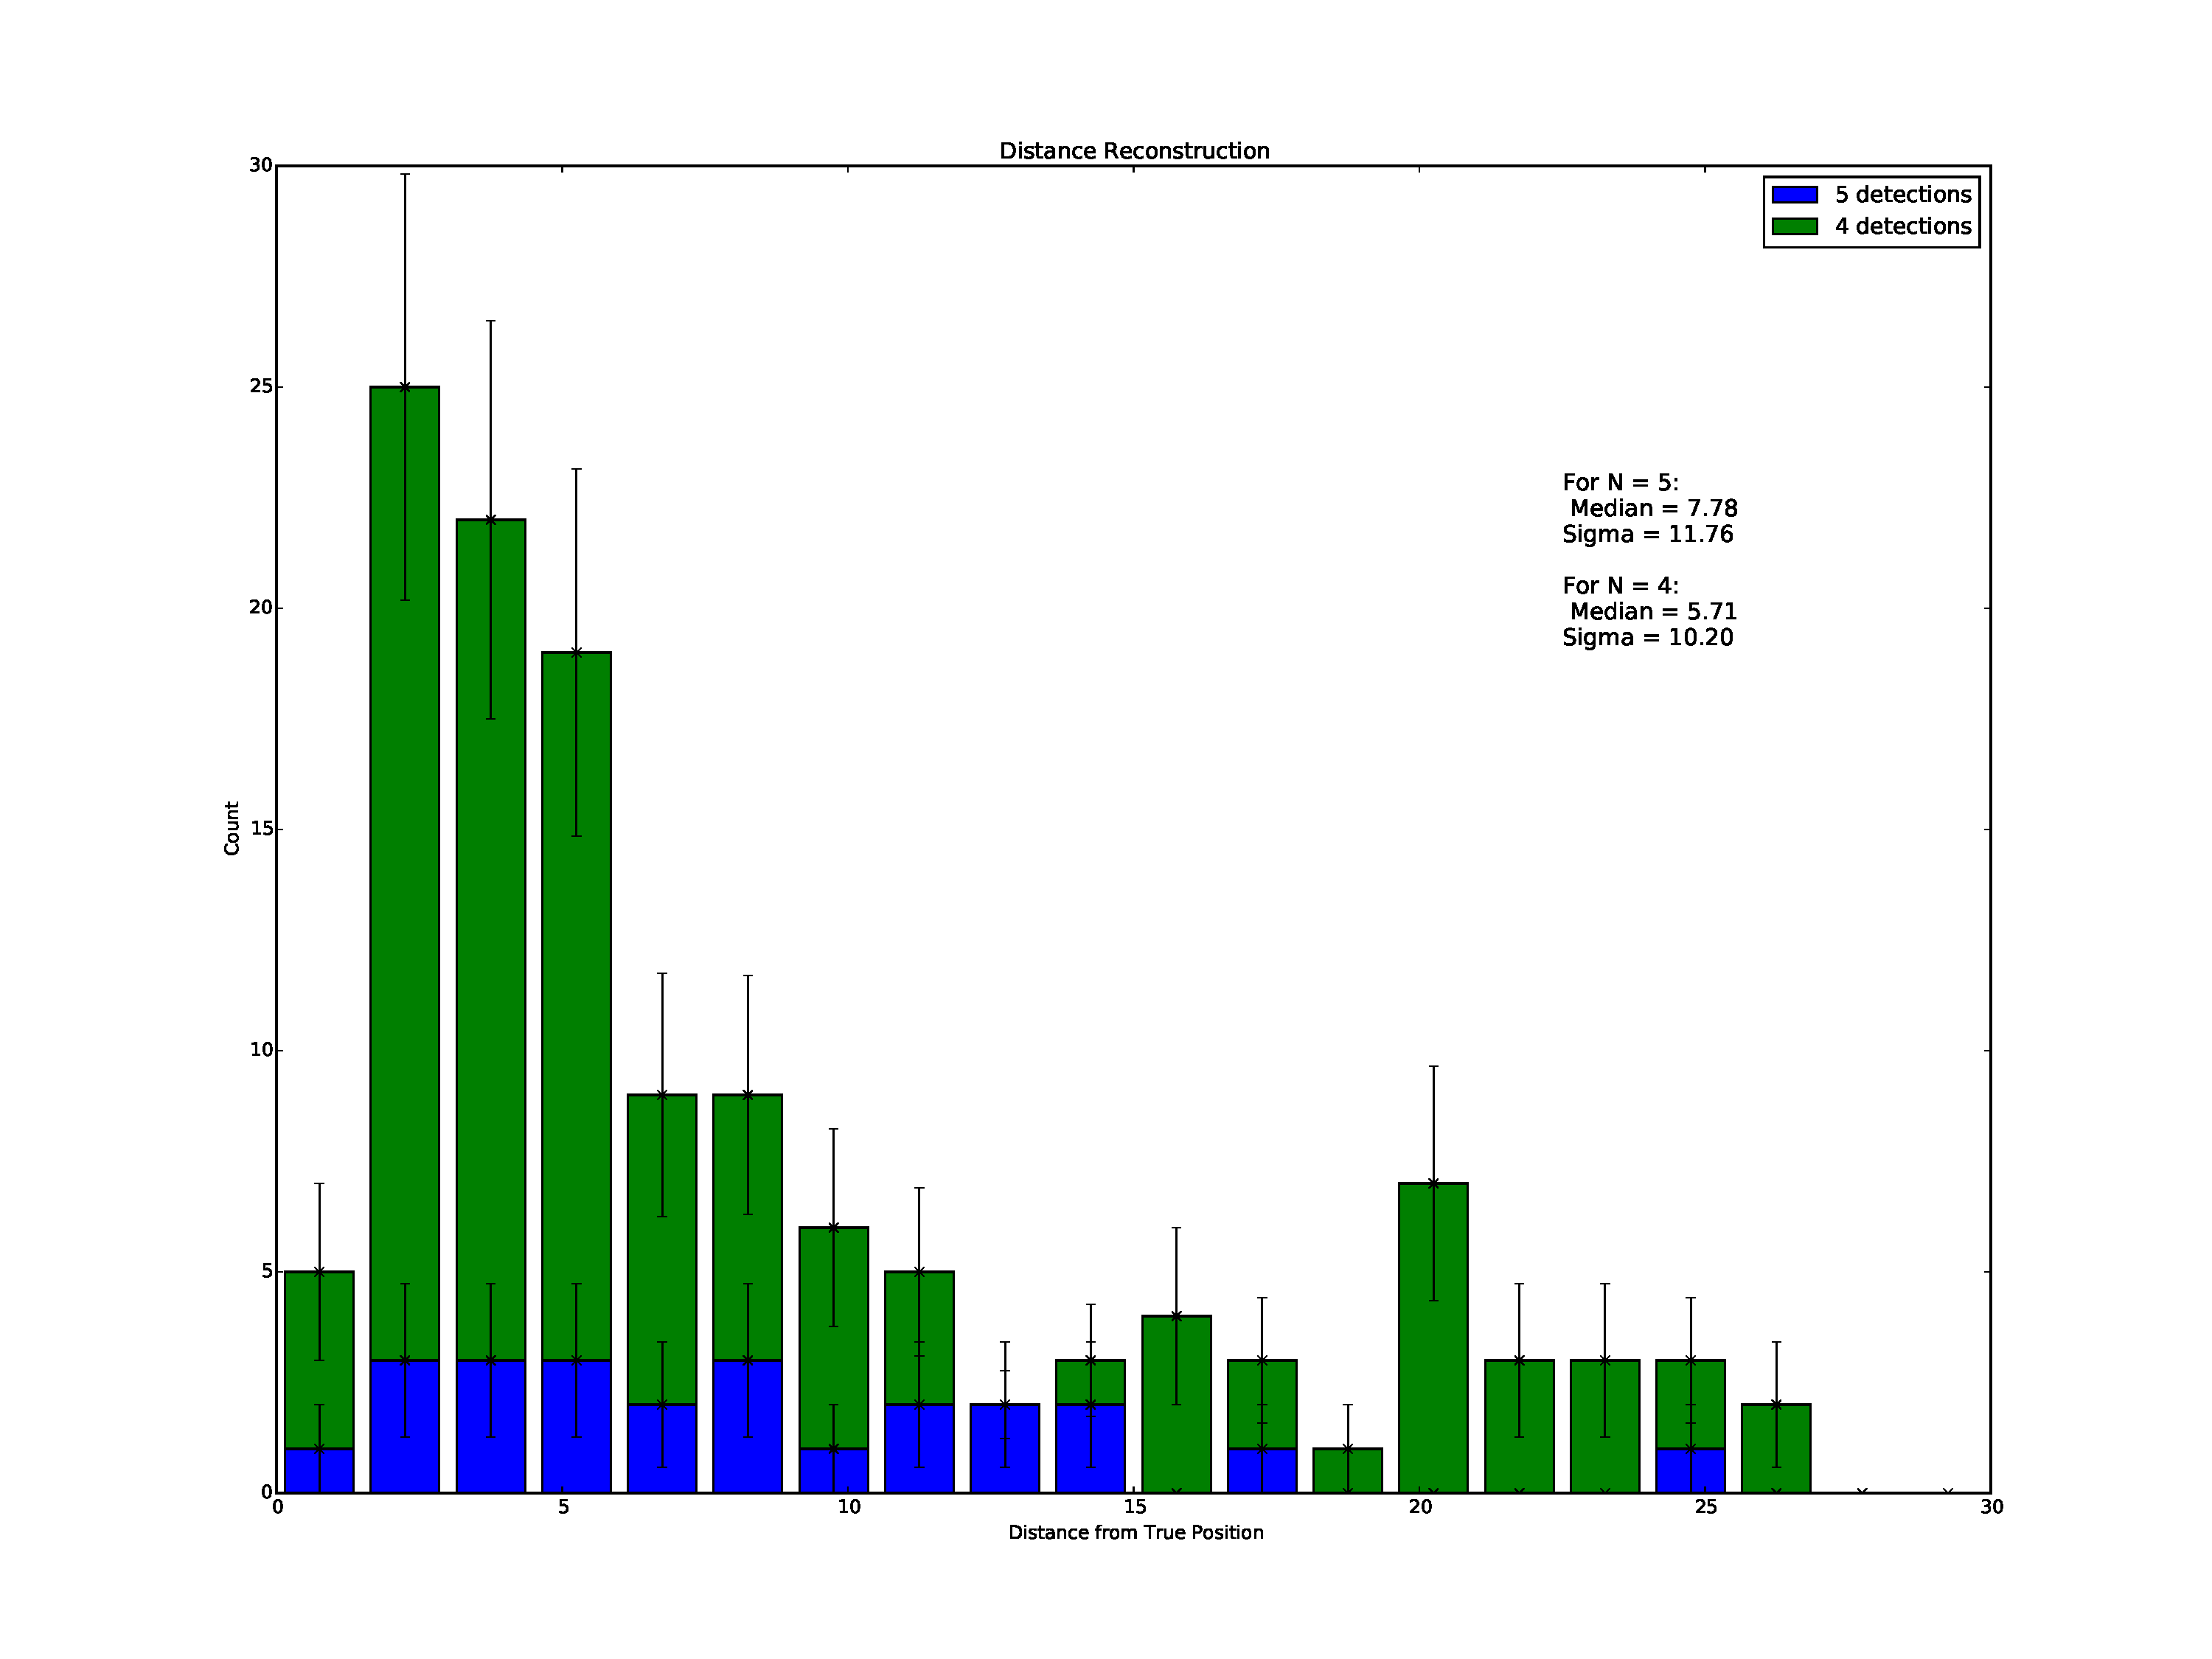
\includegraphics[width=\textwidth]{position}
\caption{The distance from true core position to the reconstructed core position is shown above. For four-telescope events, the standard deviation from true position is Xm.}
\label{fig:position}
\end{center}
\end{figure}

We can similarly consider the resolution of reconstructed height.

\begin{figure}
\begin{center}
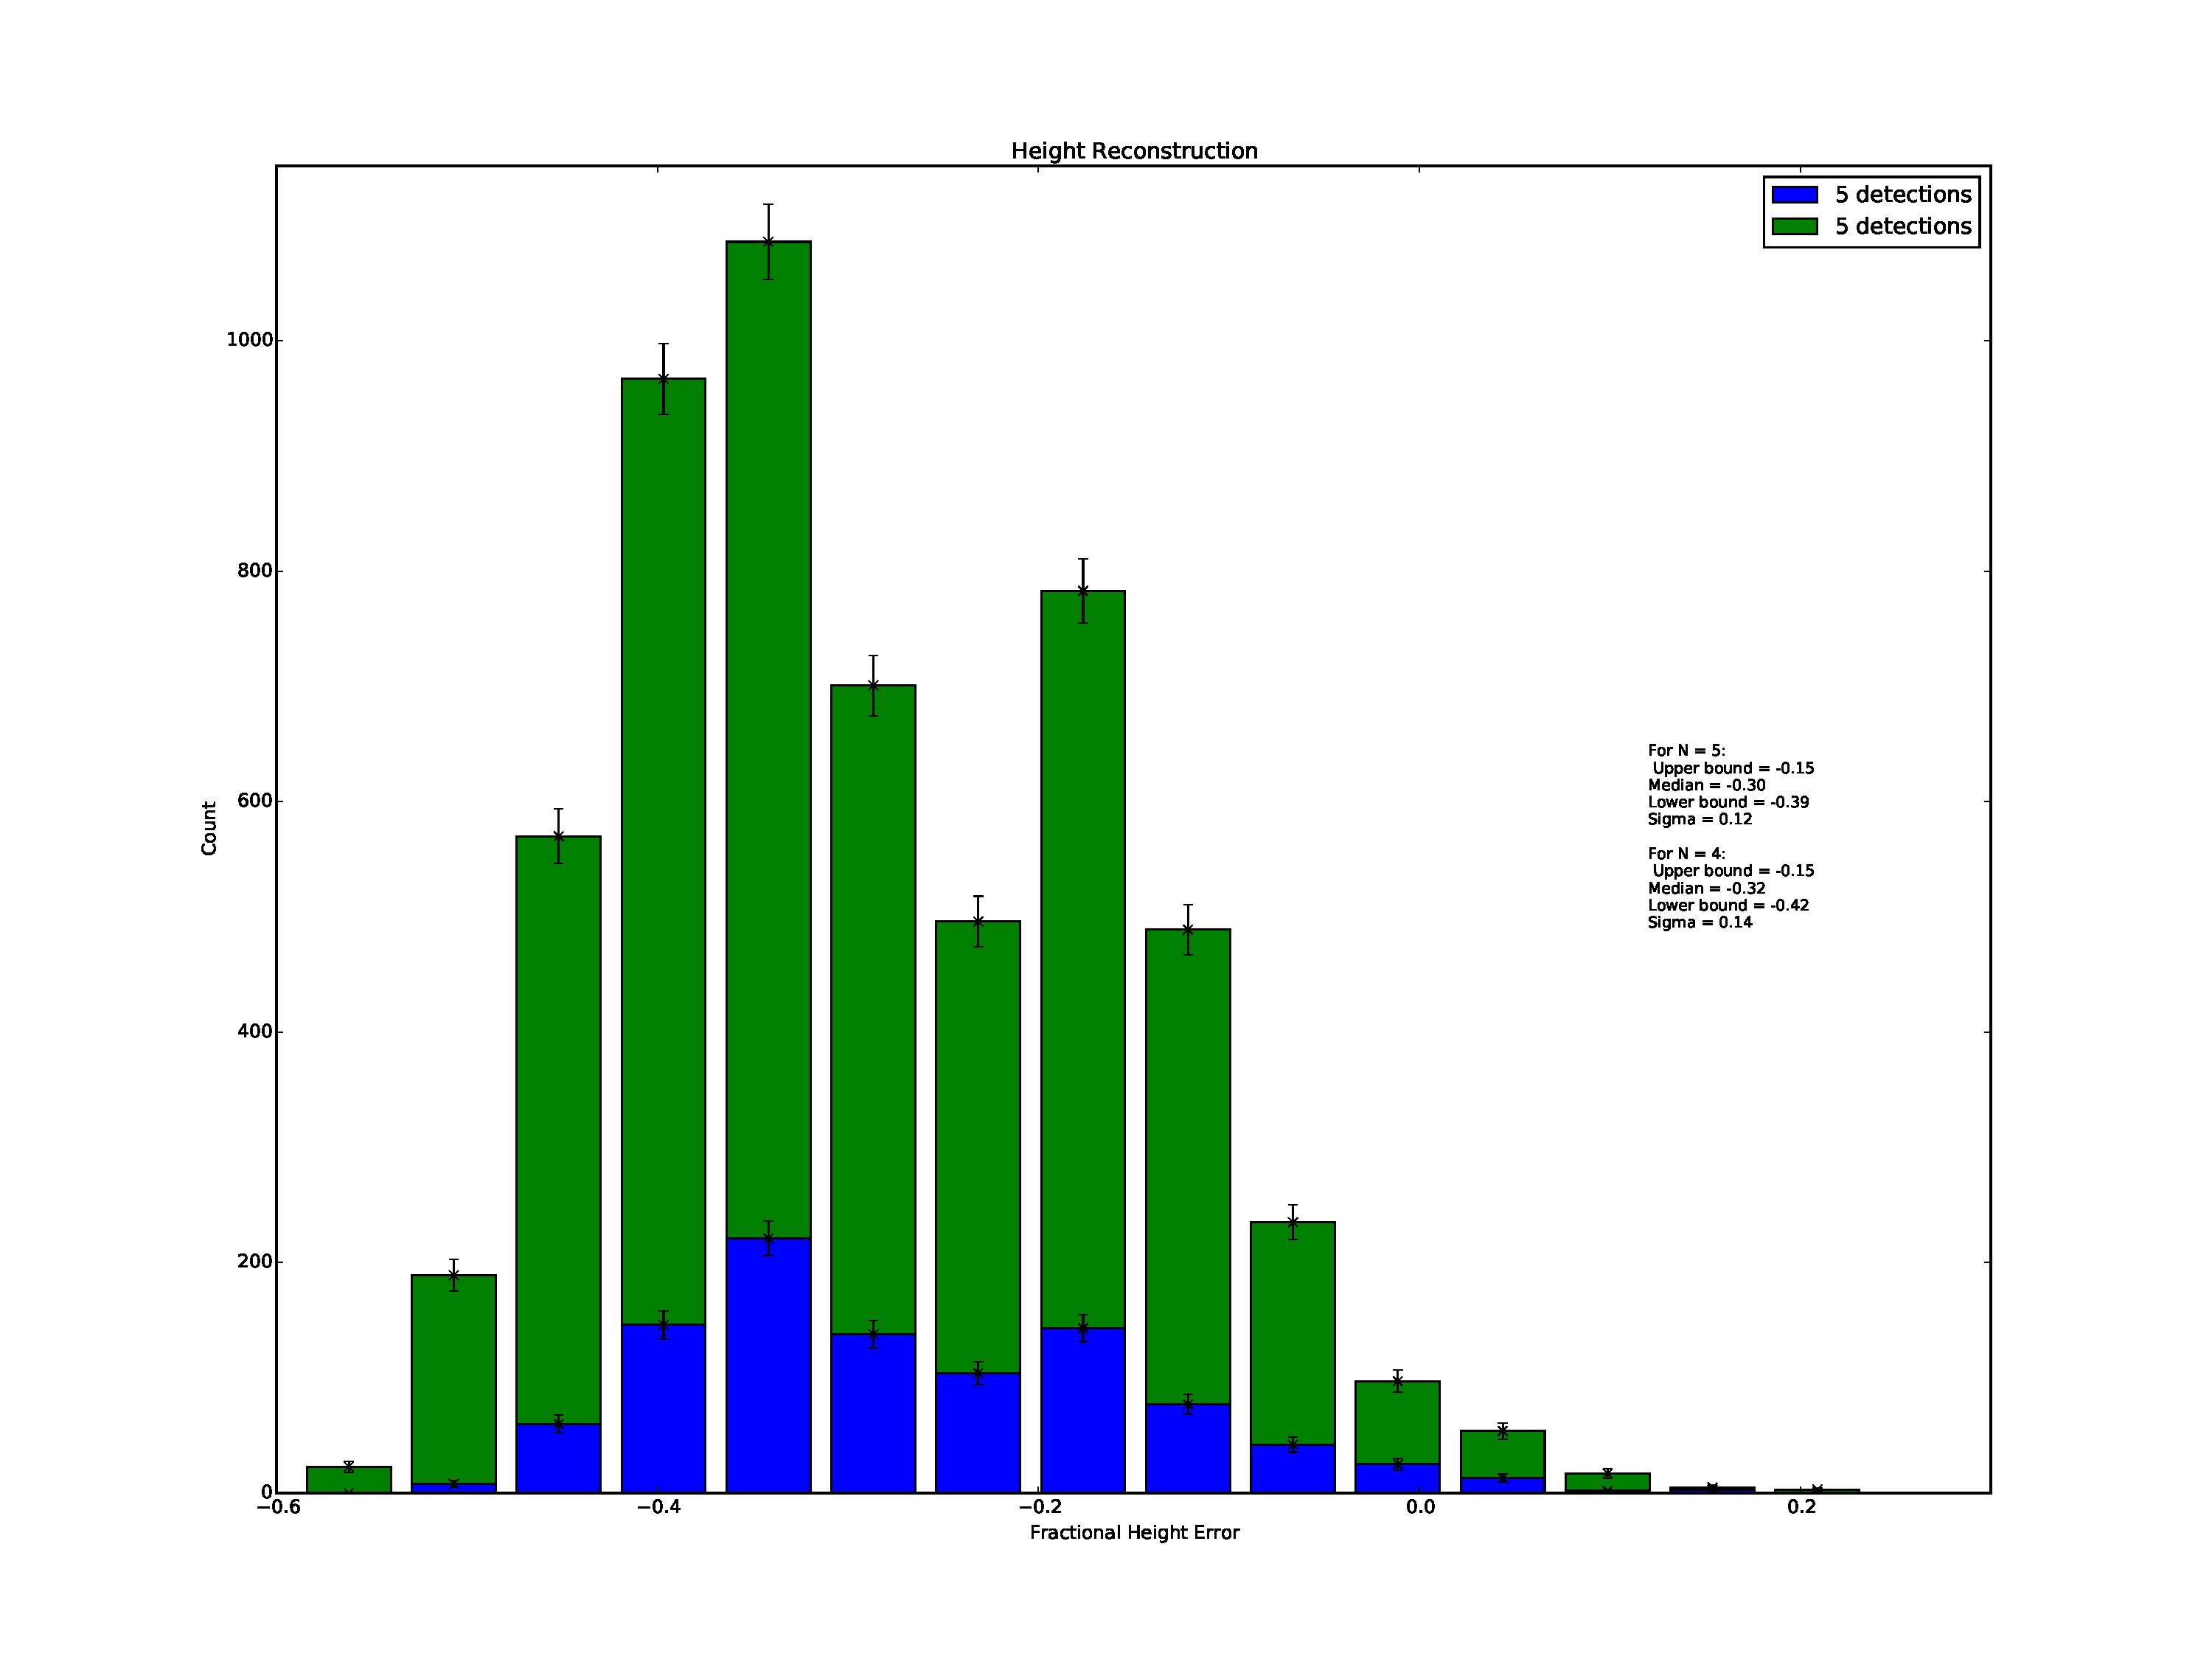
\includegraphics[width=\textwidth]{rawheight}
\caption{The distance from true core position to the reconstructed core position is shown above. For four-telescope events, the standard deviation from true position is Xm.}
\label{fig:height}
\end{center}
\end{figure}

Having taken into account our various variable uncertainties, we can also consider our most important variable. In Figure \ref{fig:rawZ} the reconstructed charge number is binned in integers, illustrating the element that each reconstructed event would be assigned to. As we would hope, there is a very clear peak centered on Z=26, and the median charge value lies very close to this value. The distributions are broadly symettric, and have a charge resoultion of $\sigma_{Z} = 1.1$ and $\sigma_{Z} = 2.2$ for five and four telescope events respectively. Unsurprisingly, the charge resolution is better for five-telescope events, but both cases represent a significant improvement over the existing charge resolution obtained through Hillas analysis. With the reasonably high event rate, we could certainly expect to see such a peak in the existing HESS data, and the uncertainty well be small enough to enable spectroscopic analysis. Obtaining such a peak is a vindication of the LPD method, and demonstrates its superior performance for event reconstruction.

\begin{figure}
\begin{center}
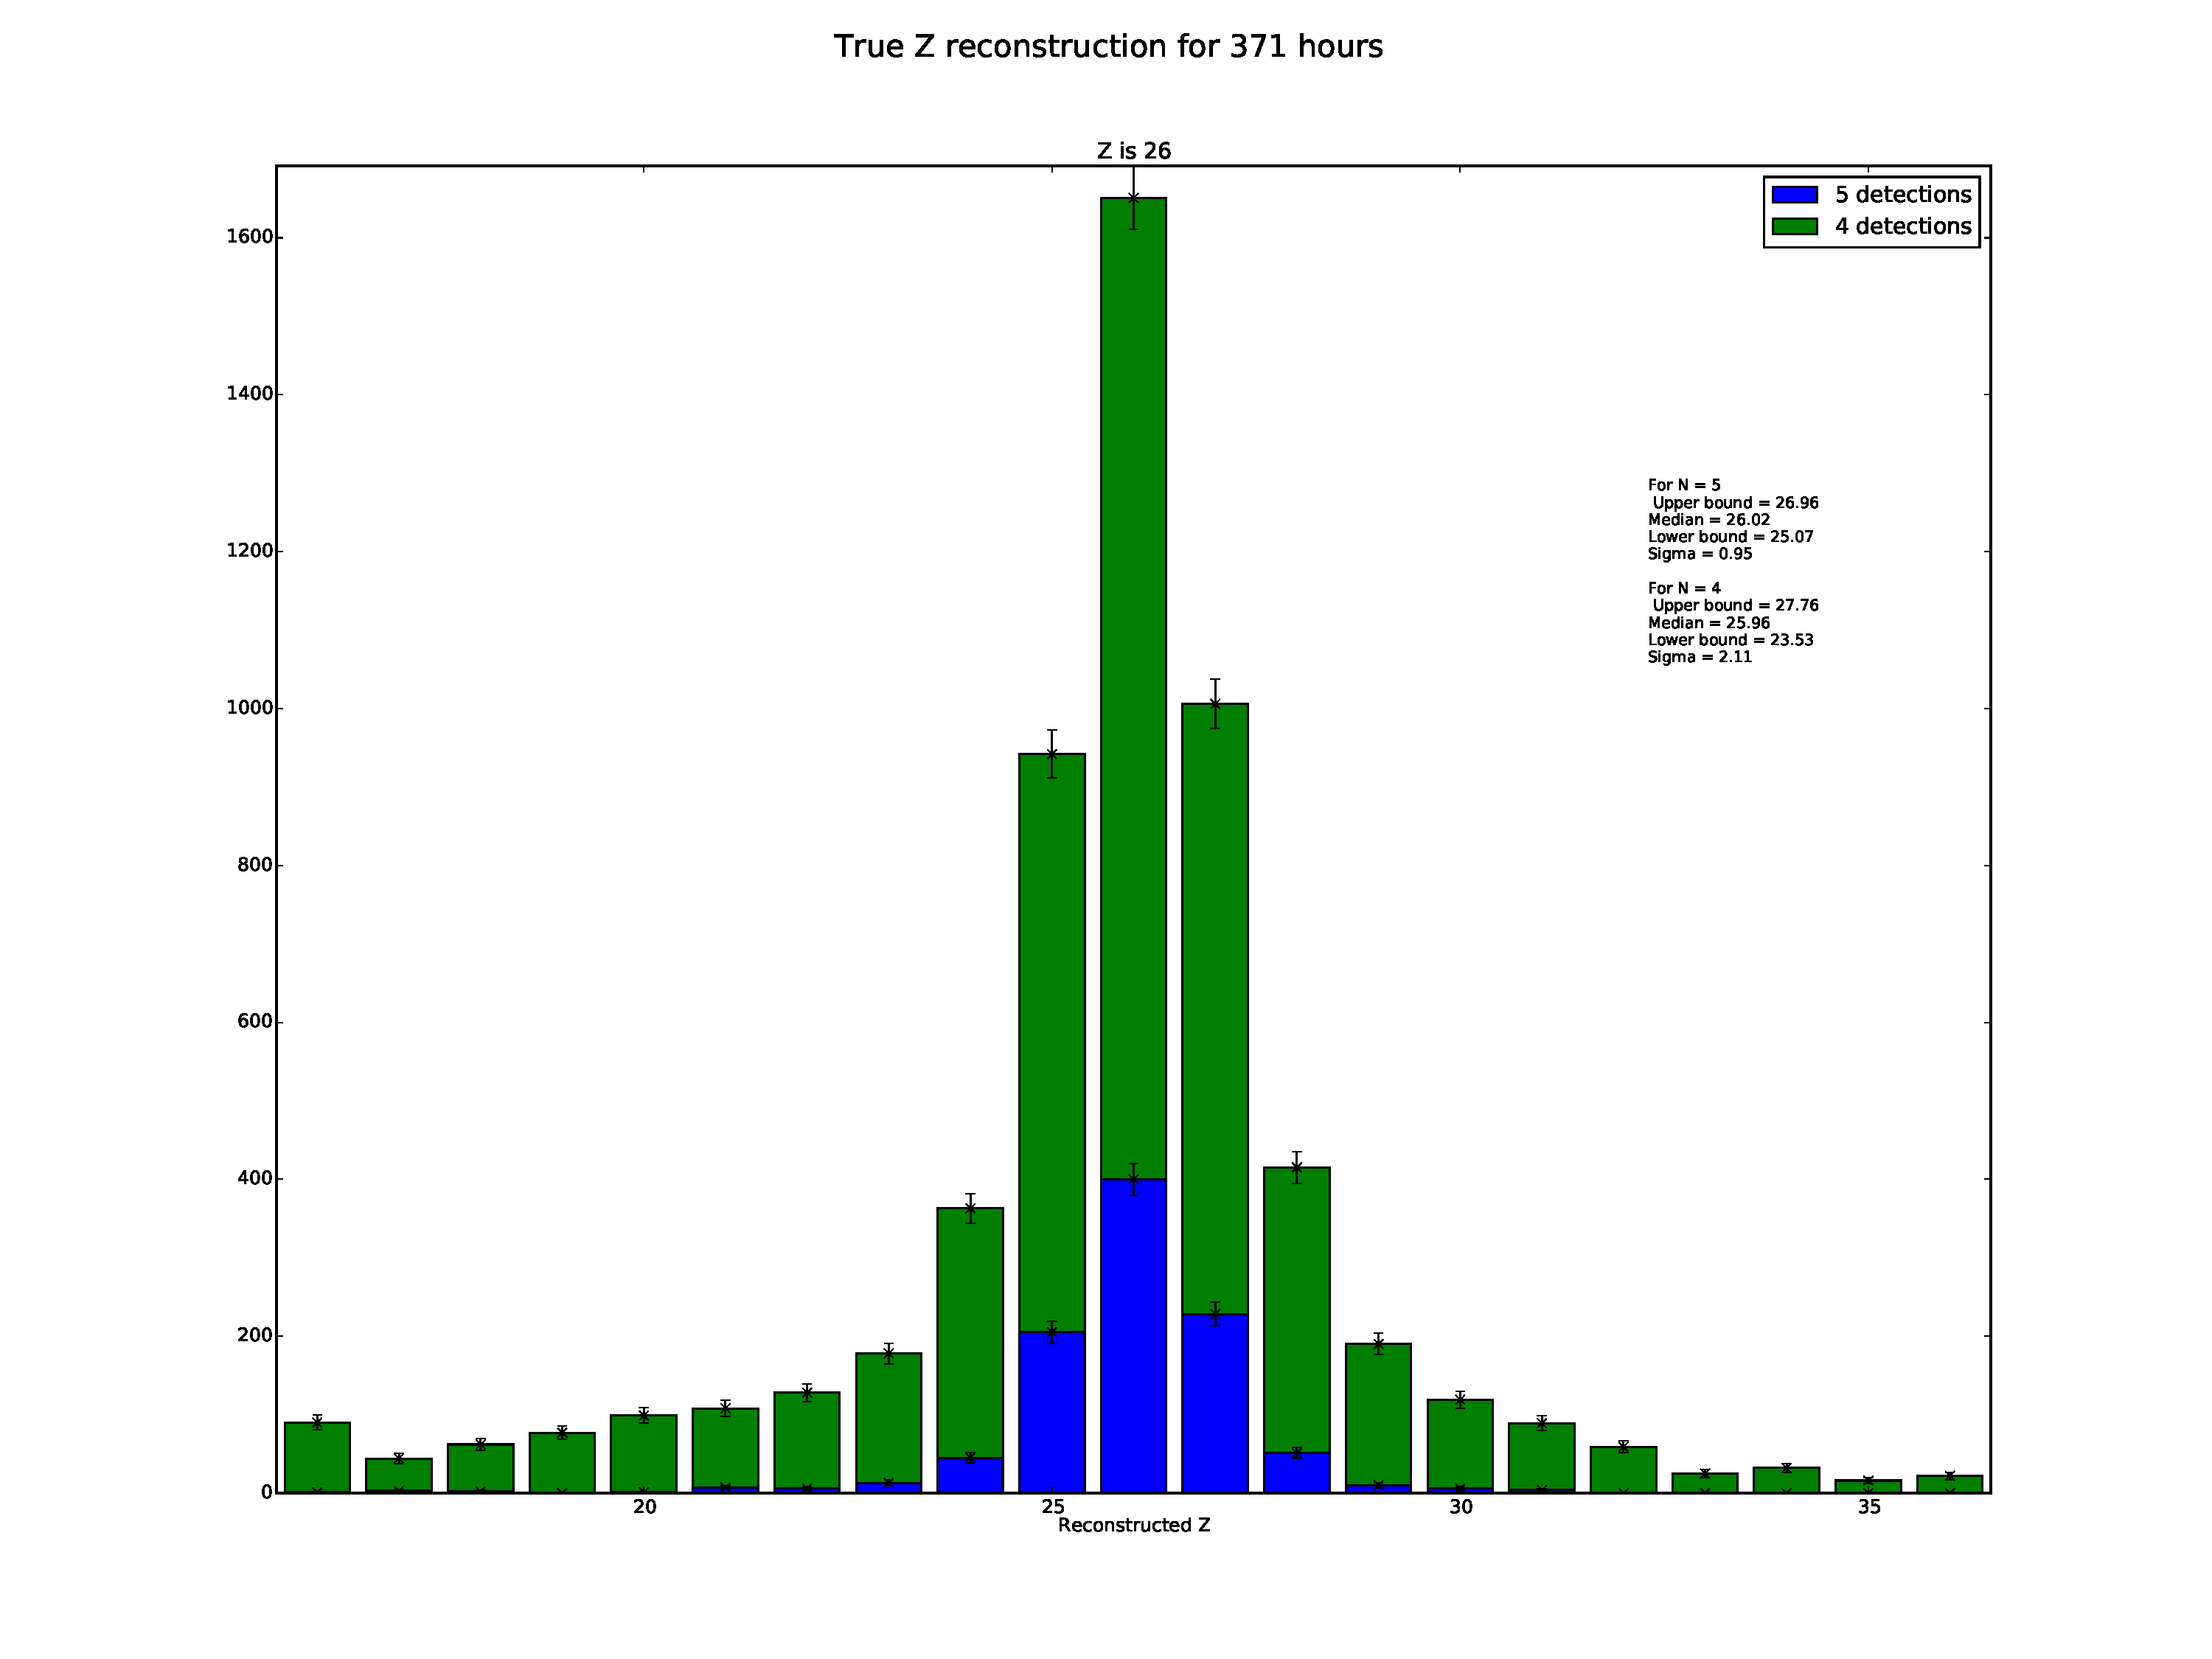
\includegraphics[width=\textwidth]{rawZ}
\caption{The distance from true core position to the reconstructed core position is shown above. For four-telescope events, the standard deviation from true position is Xm.}
\label{fig:rawZ}
\end{center}
\end{figure} 

\subsection{Boosted Decision Trees}
Using one quarter of a large sample of Monte Carlo data, we can train a Boosted Decision Tree (BDT) for a given telescope multiplicity, using the reconstructed x/y core position, height and energy, as well as the Log Likelihood. The BDT is told whether each event is \textquoteleft signal' (correctly reconstructed) or \textquoteleft background' (incorrectly reconstructed). 

For every simulated event, this trained BDT can then be used to assign a \textquoteleft Signal Probability'. On a second quarter of the dataset we can optimise a cut on the minimum signal probability, in order to maximise the ratio of signal to background. We find that the $\sigma_{Z}$ of the remaining \textquoteleft Test' Monte Carlo data is reduced when the same BDT cut is applied.

However, the simulated number of hours for the data was 1200? hours, and comparisons with HESS data show just 12 4-telescope events rather than 600. Thus, although the technique is valid and effective for HESS, the count rate will limit the potential to conduct any statistical analysis from this experiment.

\section{Optimised Telescope Array}
NO Background!!!!!
\subsection{Count Rates}

In order to improve the count rate of high-multiplicity events, we can consider a 3x3 array of Cherenkov Telescopes, which we want to use for identifying Cosmic Ray Elements accurately. In \ref{fig:optmiselayout} we see that the \textquoteleft High Multiplicity Count Rate' of events observed by 4 or more telescopes falls with increasing grid separation. We can clearly see that the optimum grid spacing will likely lie in the 20-50m region to provide a reasonable count rate. Competing with this effect is the reliance of LDF reconstruction on sampling the entire lateral distribution. Thus the reconstruction quality will decrease as Grid Width decreases. Further study of $\sigma_{Z}$ in this region is required to determine the optimum layout (not necessarily be a grid) for event reconstruction. 

\begin{figure}
\begin{center}
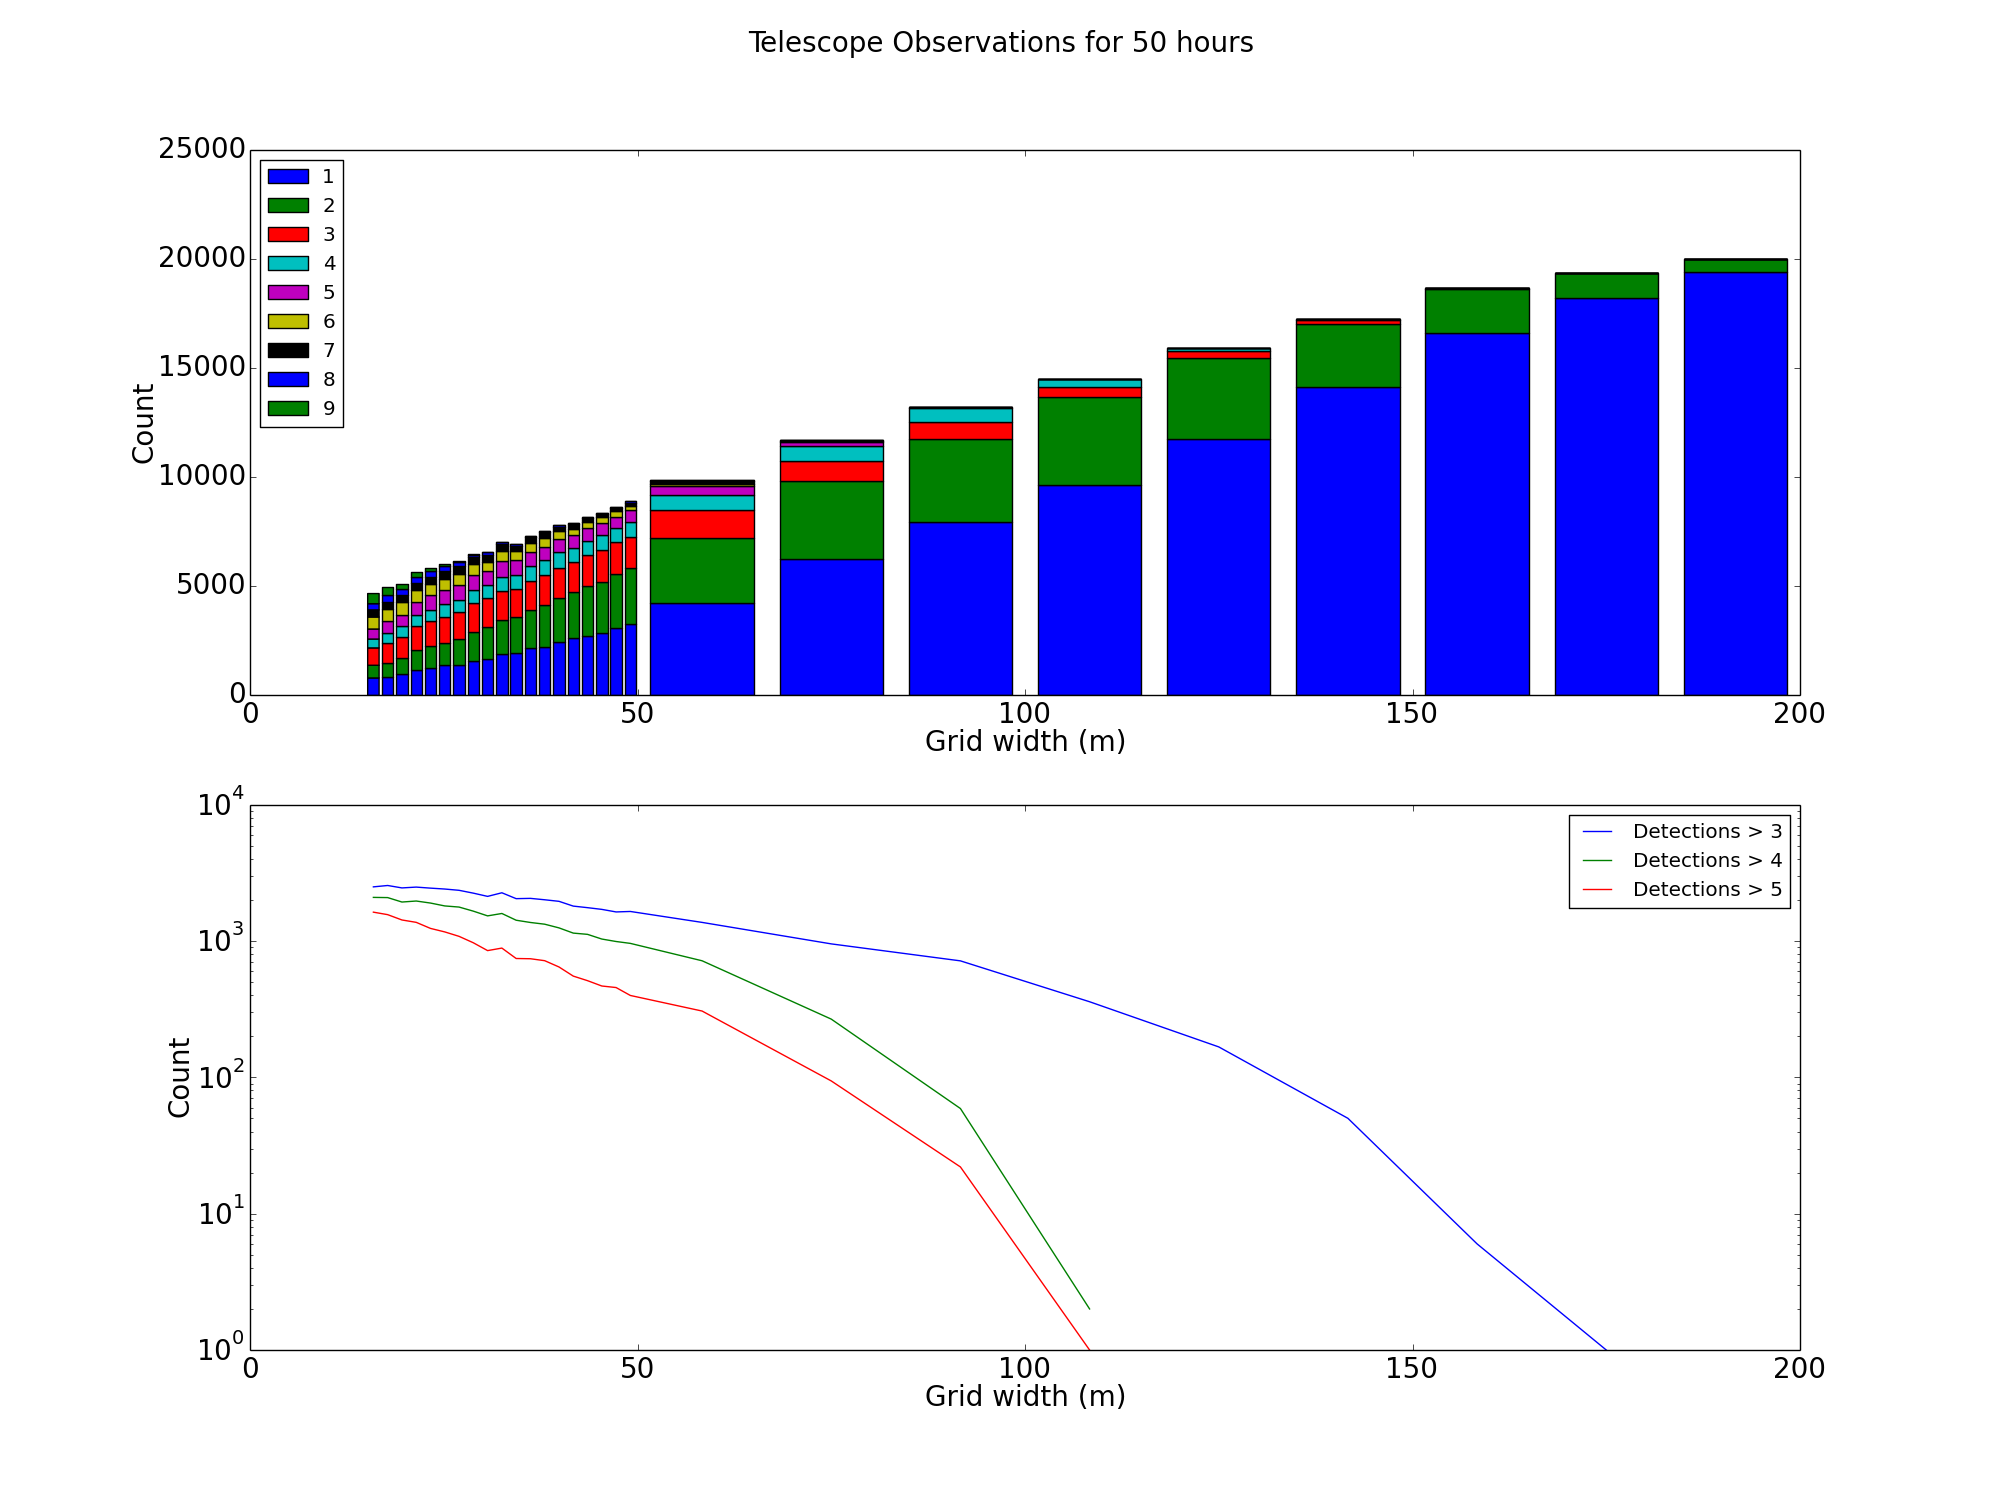
\includegraphics[width=0.9\textwidth]{optimiselayout}
\caption{A simulation of 50 hours of run time for various grid spacing for a 3x3 telescope array. Although raw count rate increases with increasing grid width, the \textquoteleft good count' rate of events observed by sufficient telescopes falls rapidly with increasing grid width}
\label{fig:optmiselayout}
\end{center}
\end{figure}

\subsection{Saturation Region Energies}
Hillas reconstruction better
Combine with Hillas reconstruction
Apply to HESS data
calibrate with position of Iron peak


\subsection{High Speed Telescopes}
By definition, the EAS shower will arrive on the ground shortly before the DC light. There are currently several high-speed Cherenkov telescopes capable of distinguishing between these, allowing a background-free LDF to be fitted. Additional study of alternative energy regimes and layouts will also be considered for the case of a high-speed imaging telescope array. 

\section{Conclusion}
Preliminary results suggest that the LDF reconstruction technique will significantly improve charge reconstruction, to a level sufficient for cosmic ray abundance studies. However, reliance on high-multiplicity events means that although applicable to current experiments such as HESS, a new optimised telescope array would be required for a statistical analysis. Such an array may have a grid spacing of 20-50m, although further study is needed to determine the ideal layout.

To get a more accurate estimate of the error, the testing set of 2000 events with varying azimuth/zenith was again considered. The fractional difference \[  \Delta = \frac{ candidate_{DC count} - True_{DC count}}{True_{DC count}} \] was binned in a histogram format, as shown in Figure \ref{fig:dcdiff}. It was observed that the mean was 0.09 and the median was -0.08, meaning the distribution was partially skewed. If the absolute deviation from the $True_{DC}$ value is considered, then 68\% of pixels have a fractional deviation less than 0.33. Accounting for $\sigma_{STA}$, we find that the $sigma_{LPD}=\sigma_{rgr1}=0.32$, an improvement over the fixed 56Tev directly incident simulation. For the high-multiplicity rejected events, we find the regressor has an error of $\sigma_{rejected1}=0.41$.

For HESS2, the mean was 0.22 while the median was -0.09, leading to an even more skewed distribution. However the 68\% absolute fractional deviation was 0.29, and with $sigma_{STA}$, we find that $sigma_{LPD}=\sigma_{rgr2}=0.29$, slightly better than for HESS1. The improved performance can be explained by the matching energy distribution for the training and testing datasets. Higher-energy events have more background EAS light without consequently increased DC light, meaning the signal becomes harder to extract. The testing dataset has predominantly low-energy events, with reduced background. For the rejected events, we find that $\sigma_{rejected2}=0.63$, with $\sigma_{STA}$ being negligible.

\begin{table}[h!]
  \centering
  \caption{Fractional error from $True_{DC}$ for all high-multiplicity test pixels}
  \label{tab:altlpderror}
  \begin{tabular}{ccc}
    \toprule
    & HESS1 & HESS2\\
    \midrule
    $\sigma_{rgr}$ & 0.32 & 0.29\\ 
    $\sigma_{rejected}$ & 0.41 & 0.63\\ 
    \bottomrule
  \end{tabular}
\end{table}

\begin{figure}
\begin{center}
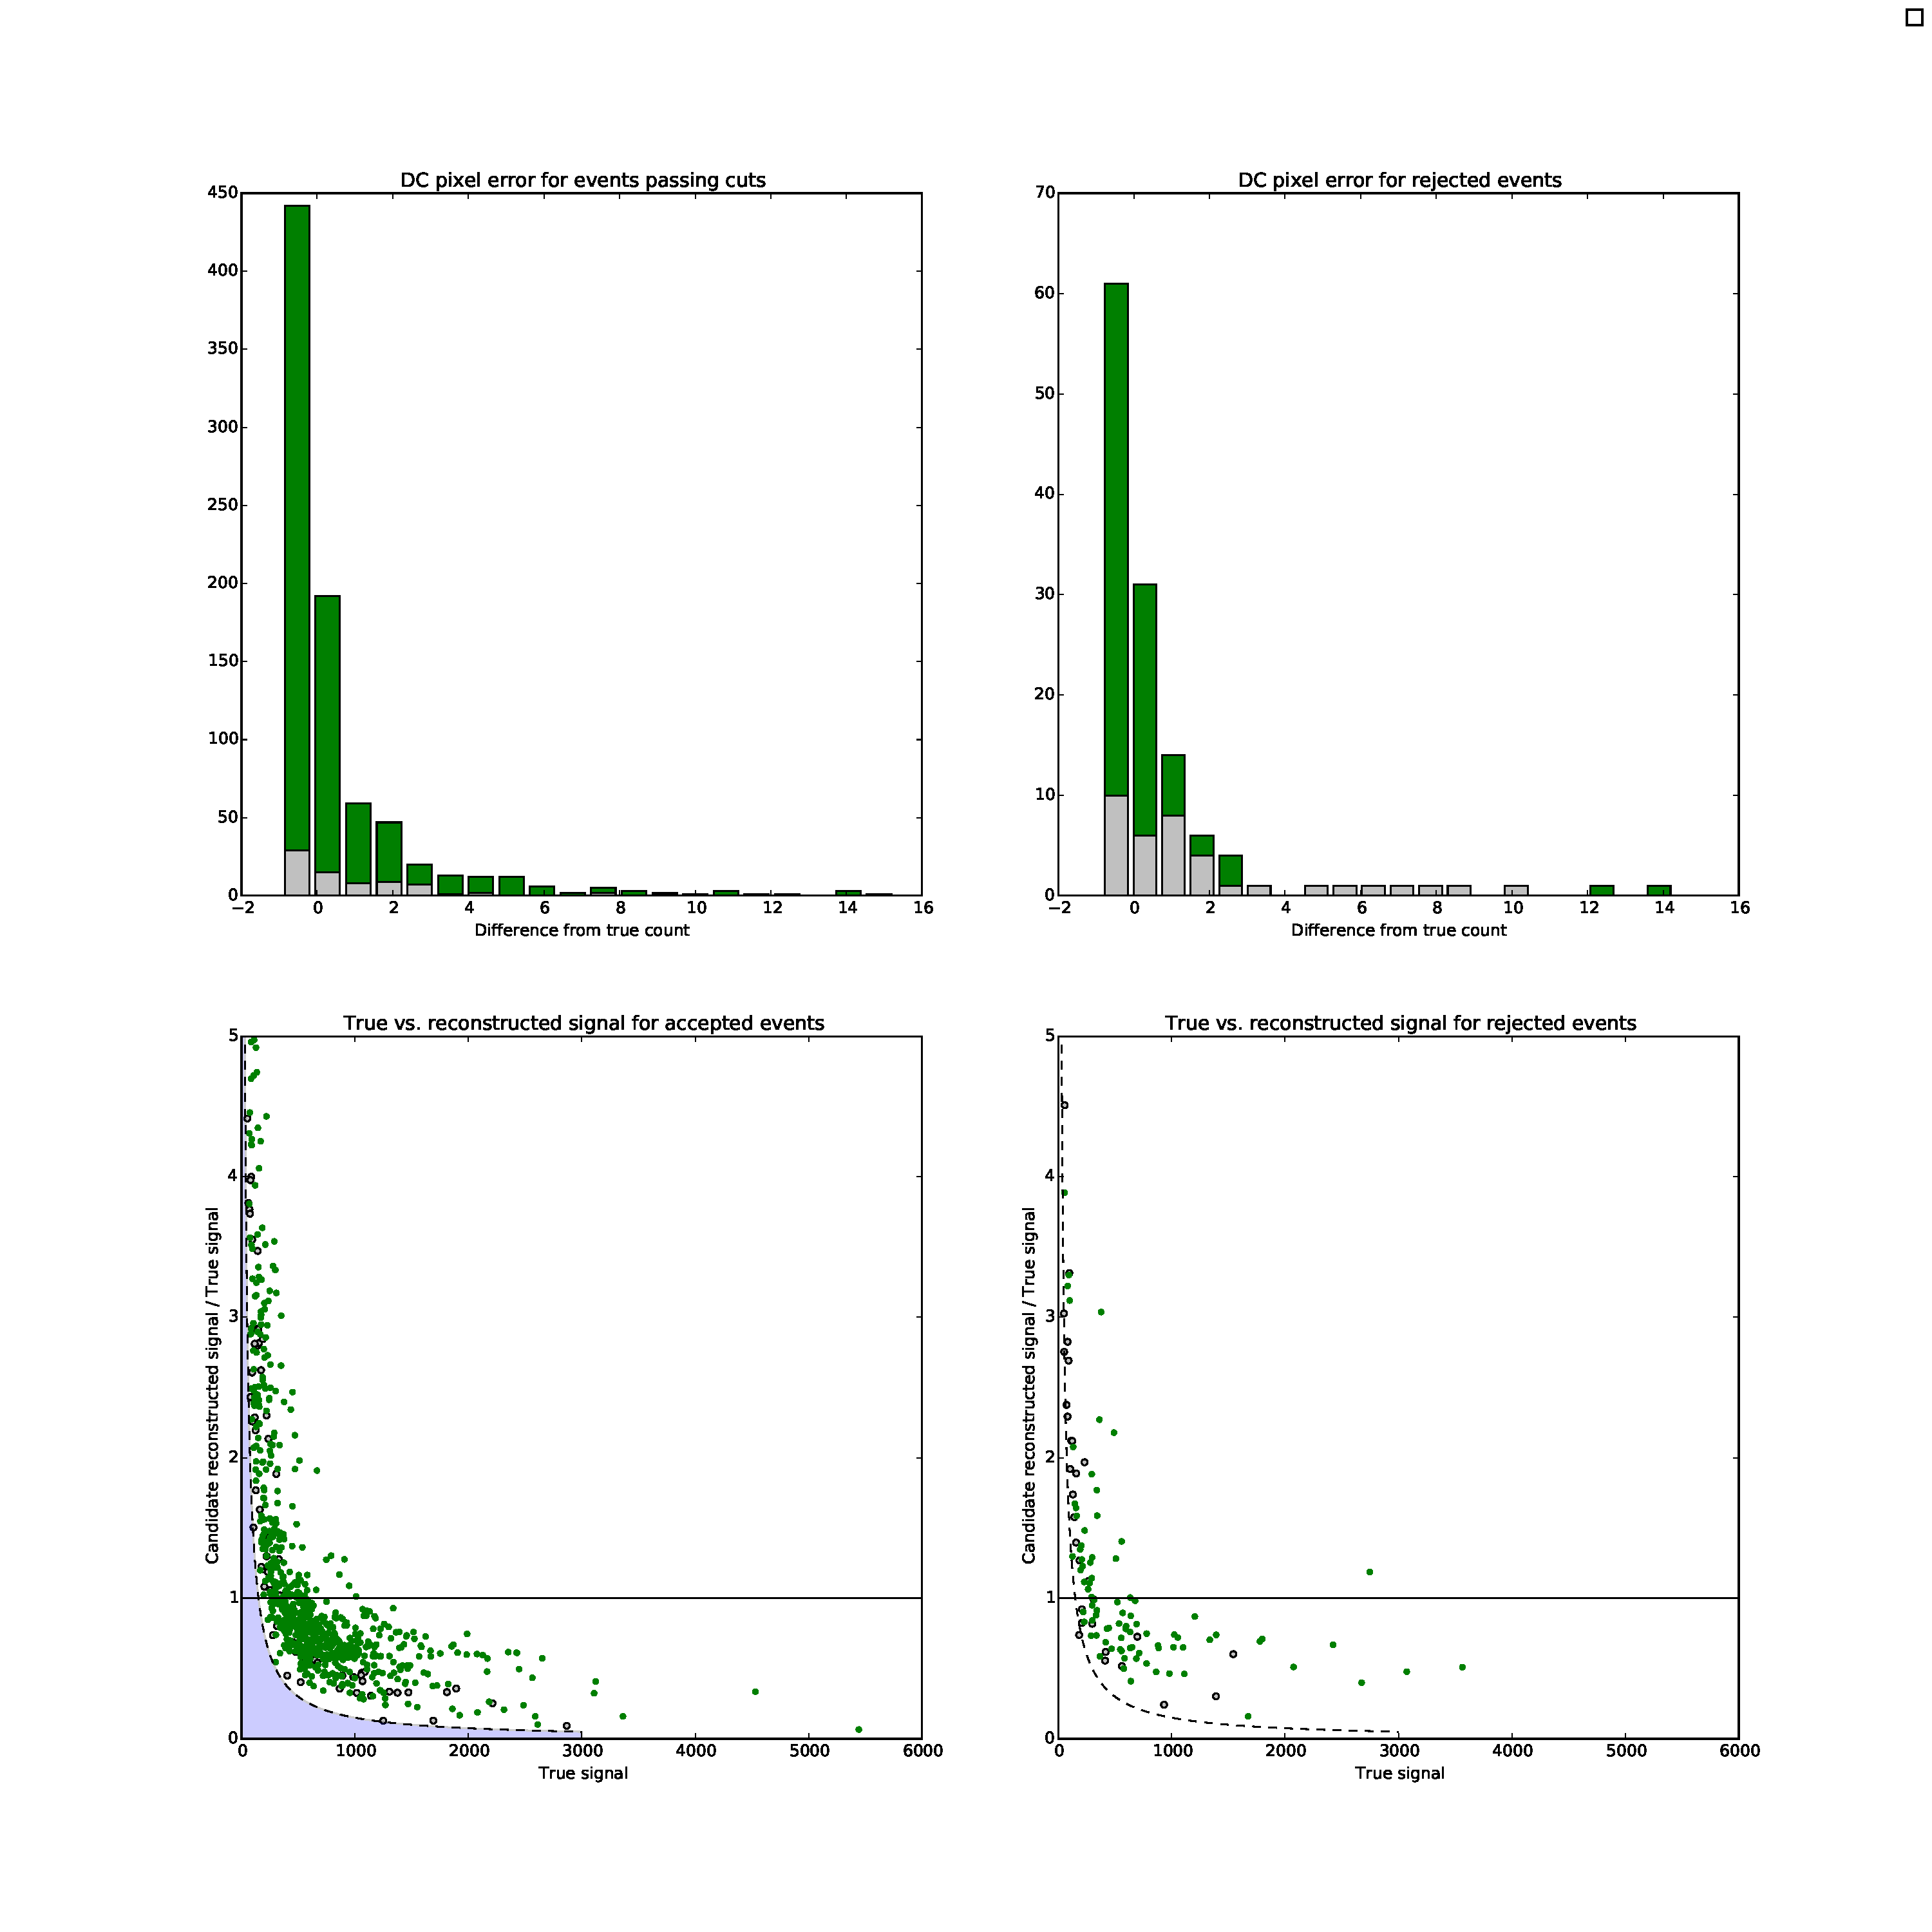
\includegraphics[width=\textwidth]{DCcounterrorhess1rgrbigtestdata}
\caption{The difference between true and reconstructed DC signal for events passing the cuts is shown in the top left. In the top right the same is shown for events which were rejected. The true DC signals for events which passed the cuts is plotted against the reconstructed signals in the lower left, and for rejected events in the lower right. As in \ref{fig:cutdistribution}, in all plots a green event is one in which the DC pixel has been correctly identified, while a red event is one that has been incorrectly identified.}
\label{fig:dcdiff}
\end{center}
\end{figure}
\section{Bibliography}
\bibliographystyle{unsrt}
\bibliography{report}
\section{Appendix}
\subsection{Atmospheric Data Table for CORSIKA (Windhoek, Namibia)}
\pgfplotstabletypeset{data/atmprof10.dat}
\end{document}